\documentclass[9pt,numbers]{sigplanconf}
\pdfpagewidth=8.5in
\pdfpageheight=11in

\usepackage[utf8]{inputenc}
\usepackage[T1]{fontenc}
\usepackage{microtype}

%
% the following standard packages may be helpful, but are not required
%
\usepackage{amsmath}
\usepackage{amssymb}
% \usepackage{SIunits}            % typset units correctly
\usepackage{courier}            % standard fixed width font
\usepackage[scaled]{helvet} % see www.ctan.org/get/macros/latex/required/psnfss/psnfss2e.pdf
\usepackage{url}                  % format URLs
\usepackage{listings}          % format code
\usepackage{enumitem}      % adjust spacing in enums
\usepackage[colorlinks=true,allcolors=blue,breaklinks,draft=false]{hyperref}   % hyperlinks, including DOIs and URLs in bibliography
% known bug: http://tex.stackexchange.com/questions/1522/pdfendlink-ended-up-in-different-nesting-level-than-pdfstartlink
\newcommand{\doi}[1]{doi:~\href{http://dx.doi.org/#1}{\Hurl{#1}}}   % print a hyperlinked DOI
\usepackage{xspace}
\usepackage{commands}
\usepackage{graphicx}
%\usepackage{pdfpages}
%\usepackage[doi]{natbib}

\usepackage{amsthm}
\renewcommand{\qedsymbol}{\ensuremath{\blacksquare}}
% \newtheorem{lemma}{Lemma}
% \newtheorem{corollary}{Corollary}
% \newtheorem{theorem}{Theorem}
% \newtheorem{definition}{Definition}
\theoremstyle{plain}% default
\newtheorem{thm}{Theorem} % [section]
\newtheorem{lem}[thm]{Lemma}
\newtheorem{prop}[thm]{Proposition}
\newtheorem*{cor}{Corollary}
\theoremstyle{definition}
\newtheorem{defn}{Definition} % [section]

\usepackage{pgfplots}
\usepackage{pgfkeys}
\pgfplotsset{compat=1.12}

\usepackage[inference]{semantic}


\usepackage{ifthen}
\newcommand{\isTechReport}{false} % true or false
\newcommand\includeTechReport[1]{%
  \ifthenelse{\equal{\isTechReport}{true}}
    {{#1}}
    {\ignorespaces}
\xspace}

%% avoid orphan text and headings
\clubpenalty=10000
\widowpenalty=10000
\displaywidowpenalty=10000

%% balance columns on final page
\usepackage{flushend}

%% bibliography
%% \usepackage[backend=biber,isbn=false,firstinits=true,style=trad-abbrv]{biblatex}
%% \addbibresource{main.bib}

\begin{document}
\toappear{}

\title{Dynamic Witnesses for Static Type Errors}

\subtitle{(or, ill-typed programs \emph{usually} go wrong)}

\authorinfo{Eric L. Seidel \and Ranjit Jhala}
           {UC San Diego}
           {\{eseidel,rjhala\}@cs.ucsd.edu}

\authorinfo{Westley Weimer}
           {University of Virginia}
           {weimer@viginia.edu}

\maketitle

%\usepackage{listings}
%
%\usepackage{color}
% uncomment next line to restore colors
% \def\withcolor{}

\ifdefined\withcolor
	\definecolor{haskellblue}{rgb}{0.0, 0.0, 1.0}
	\definecolor{haskellstr}{rgb}{0.2, 0.2, 0.6}
	\definecolor{haskellred}{rgb}{1.0, 0.0, 0.0}
	\definecolor{gray_ulisses}{gray}{0.55}
	\definecolor{castanho_ulisses}{rgb}{0.71,0.33,0.14}
	\definecolor{preto_ulisses}{rgb}{0.41,0.20,0.04}
	\definecolor{green_ulisses}{rgb}{0.0,0.4,0.0}
\else
	\definecolor{haskellblue}{gray}{0.1}
	\definecolor{haskellstr}{gray}{0.1}
	\definecolor{haskellred}{gray}{0.1}
	\definecolor{gray_ulisses}{gray}{0.1}
	\definecolor{castanho_ulisses}{gray}{0.1}
	\definecolor{preto_ulisses}{gray}{0.1}
	\definecolor{green_ulisses}{gray}{0.1}
\fi


\def\codesize{\normalsize}

\lstdefinelanguage{HaskellUlisses}{
	basicstyle=\ttfamily,
	sensitive=true,
	morecomment=[l][\color{gray_ulisses}\ttfamily]{--},
	morecomment=[s][\color{gray_ulisses}\ttfamily]{\{-}{-\}},
	morestring=[b]",
	stringstyle=\color{haskellstr},
	showstringspaces=false,
	numberstyle=\codesize,
	numberblanklines=true,
	showspaces=false,
	breaklines=true,
	showtabs=false,
        escapeinside={(*}{*)},%
        % mathescape=true,
	emph=
	{[1]
		FilePath,IOError,abs,acos,acosh,and,any,appendFile,approxRational,asTypeOf,asin,
		asinh,atan,atan2,atanh,basicIORun,break,catch,ceiling,chr,compare,concat,concatMap,
		const,cos,cosh,curry,cycle,decodeFloat,denominator,digitToInt,div,divMod,drop,
		dropWhile,either,elem,encodeFloat,enumFrom,enumFromThen,enumFromThenTo,enumFromTo,
		error,even,exp,exponent,fail,filter,flip,floatDigits,floatRadix,floatRange,floor,
		fmap,foldl,foldl1,foldr,foldr1,fromDouble,fromEnum,fromInt,fromInteger,
		fromRational,fst,gcd,getChar,getContents,getLine,head,id,inRange,index,init,intToDigit,
		interact,ioError,isAlpha,isAlphaNum,isAscii,isControl,isDenormalized,isDigit,isHexDigit,
		isIEEE,isInfinite,isLower,isNaN,isNegativeZero,isOctDigit,isPrint,isSpace,isUpper,iterate,
		last,lcm,length,lex,lexDigits,lexLitChar,lines,log,logBase,lookup,mapM,mapM_,max,
		maxBound,maximum,maybe,min,minBound,minimum,mod,negate,not,notElem,numerator,odd,
		or,pi,primExitWith,print,product,properFraction,putChar,putStr,putStrLn,quot,
		quotRem,range,rangeSize,read,readDec,readFile,readFloat,readHex,readIO,readInt,readList,readLitChar,
		readLn,readOct,readParen,readSigned,reads,readsPrec,realToFrac,recip,rem,repeat,
		reverse,round,scaleFloat,scanl,scanl1,scanr,scanr1,seq,sequence,sequence_,show,showChar,showInt,
		showList,showLitChar,showParen,showSigned,showString,shows,showsPrec,significand,signum,sin,
		sinh,snd,span,splitAt,sqrt,subtract,succ,sum,tail,take,takeWhile,tan,tanh,threadToIOResult,toEnum,
		toInt,toInteger,toLower,toRational,toUpper,truncate,uncurry,undefined,unlines,until,unwords,unzip,
		unzip3,userError,words,writeFile,zip,zip3,zipWith,zipWith3,listArray,doParse,for,initTo,
                create,get,set,div,rescale,add,delete,insert,prop_focus_left_master,average,best,insert,union,split,size,fromList,copy,group,good,bad,foo,explode,singleton,difference,fromJust,sort,unfold,
                subst,unapply,apply,proxy,refinement,fresh,guard,constrain,oneOf,
                queryList,queryCtor,queryField,ctors,decodeCtor,whichOf,ctorArity,eval,
                mkCtor,gCtors,gEncode,gEncodeFields,gDecode,gDecodeFields,reproxyRep,empty,splitCtor,checkField,scanM,
                padAverage,focusUp,execute,checkSMT,inputTypes,outputType,toReft,app,
                genArgs,genWitness,close,witness,mkApps,mkLets,isStuck,findExpr,updState,putBefore,putAfter,
                putRoot,getNext,getPrev,getSubterms,applyCtx,findApp,findVal,replicate,loop,fac,incAllByOne,map
                %, inTypes, inputTypes, outputType, execute, smtFindModel, smtRefuteModel
	},
	emphstyle={[1]\color{haskellblue}},
	emph=
	{[2]
		OkMap,OkRBT,OkStackSet,TTrue,Map,Bool,Char,Double,Either,Float,IO,Integer,Int,Maybe,Ordering,Rational,Ratio,ReadS,ShowS,String,Word8,Nat,Pos,Rng,Score,
                Ptr,ForeignPtr,CSize,InPacket,Tree,Prop,TreeEq,TreeLt,Vec,
                NullTerm,IncrList,DecrList,UniqList,BST,MinHeap,MaxHeap,
                PtrN,ByteStringN,ByteStringEq,VO,ByteStringsEq,ByteStringNE,OrdList,Var,RType,Constrain,Gen,Var,Proxy,SMT,Targetable,RefType,Refinement,Ctor,C1,Rep,Rec0,U1,
                GCtors,GDecode,GDecodeFields,GEncode,GEncodeFields,OrdMap,MinusKey,
                len,isBH,isBal,bh,isRB,keys,Sorted,RBT,Col,isBlack,OrdRBT,Set,sz,
                StackSet,NoDuplicates,Data,RBTree,XMonad,Generic,
                VState,Expr,Ctx,Cmd,int,list,string,bool
	},
	emphstyle={[2]\color{castanho_ulisses}},
	emph=
	{[3]
		case,class,data,deriving,do,else,if,return,def,import,in,infixl,infixr,instance,let,tmapM,for2M,forM,zipWithM,otherwise,
		module,measure,pred,predicate,of,primitive,then,type,where,lazy,throw,when,
                rec,function,fun,match,with
	},
	emphstyle={[3]\color{preto_ulisses}\textbf},
	emph=
	{[4]
		quot,rem,div,mod,elem,notElem,seq
	},
	emphstyle={[4]\color{castanho_ulisses}\textbf},
	emph=
	{[5]
		PS,Tip,Node,Black,Red,EQ,False,GT,Just,LT,Left,Nothing,Right,True,Show,Eq,Ord,Num,C,N,Leaf,Bin,CounterExample,
                StepForward,StepBack,JumpForward,JumpBack,StepOver,StepInto,true
	},
	emphstyle={[5]\color{green_ulisses}},
	emph=
	{[6]
		patError, irrefutPatError, nonExhaustiveGuardsError, recSelError, errorOut,
		noMethodBinding
	},
	emphstyle={[6]\color{haskellred}}
}

%%%ORIG
%%%\lstnewenvironment{code}
%%%{\textbf{Haskell Code} \hspace{1cm} \hrulefill \lstset{language=HaskellUlisses}}
%%%{\hrule\smallskip}

%V1
%\lstnewenvironment{code}
%{\smallskip \lstset{language=HaskellUlisses}}
%{\smallskip}

\lstdefinelanguage{HaskellUlissesMath}[]{HaskellUlisses}{mathescape=true}

\lstnewenvironment{code}
{\lstset{language=HaskellUlisses}}
{}

\lstnewenvironment{mcode}
{\lstset{language=HaskellUlissesMath}}
{}

\lstnewenvironment{fcode}
{\lstset{language=HaskellUlisses, frame=L}}
{}

\lstMakeShortInline[language=HaskellUlisses]@
\lstMakeShortInline[language=HaskellUlissesMath]|


\begin{abstract}
  %
  \emph{Static} type errors are a common stumbling block
  for newcomers to typed functional languages.
  %
  We present a \emph{dynamic} approach to explaining type
  errors by generating counterexample witness inputs that
  illustrate \emph{how} an ill-typed program goes wrong.
  %
  First, given an ill-typed function, we first symbolically
  execute the body to dynamically synthesize witness values
  that can make the program go wrong.
  We prove that our procedure synthesizes
  \emph{general witnesses} in that if a witness is
  found, then \emph{for all} input types, there exist
  inhabitants that can make the function go wrong.
  %
  Second, we show how to extend the above procedure to
  produce a \emph{reduction graph} that can be used to
  interactively visualize and debug witness executions.
  %
  Third, we evaluate our approach on two data sets
  comprising over 4,500 ill-typed student programs.
  Our technique is able to generate witnesses for
  88\% of the programs, and our reduction graph
  is yields small counterexamples for 90\% of the witnesses.
\end{abstract}


\category{D.3.2}
         {Programming Languages}
         {Language Classifications}
         [Applicative (functional) languages]
\category{D.3.4}
         {Programming Languages}
         {Processors}
         [Debuggers]
\category{F.3.3}
         {Logics and Meanings of Programs}
         {Studies of Program Constructs}
         [Type structure]
\terms
Languages
\keywords
debugging, testing, type errors

\section{Introduction}
\label{sec:introduction}

Type errors are a common stumbling block for students
trying to learn typed functional languages like \ocaml\
and \haskell.
%
Consider the ill-typed @fac@ function on the left in
Figure~\ref{fig:factorial}.
%
The function returns @true@ in the base case (instead of @1@),
and so \ocaml responds with the error message:
%
\begin{verbatim}
 File "fac.ml", line 5, characters 8-23:
 Error: This expression has type bool
        but an expression was expected
        of type int
\end{verbatim}
%
This message makes perfect sense to an expert who is familiar
with the language and has a good mental model of how the type
system works.
%
However, it may perplex a novice who has yet to develop such a
mental model.
%
To make matters worse, unification-based type inference algorithms
often report errors far removed from their source.
%
This further increases the novice's confusion and can actively mislead
them to focus their investigation on an irrelevant piece of code.
%
Much recent work has focused on analyzing unification constraints
to properly \emph{localize} a type error~\cite{lerner_searching_2007,chen_counter-factual_2014,zhang_toward_2014,pavlinovic_finding_2014},
but an accurate source location still does not explain \emph{why} the
program is wrong.


\begin{figure}[t]
\centering
\begin{minipage}{.49\linewidth}
\begin{code}
let rec fac n =
  if n <= 0 then
    true
  else
    n * fac (n-1)
\end{code}
\end{minipage}
\hspace{0.3in}
\begin{minipage}{.3\linewidth}
  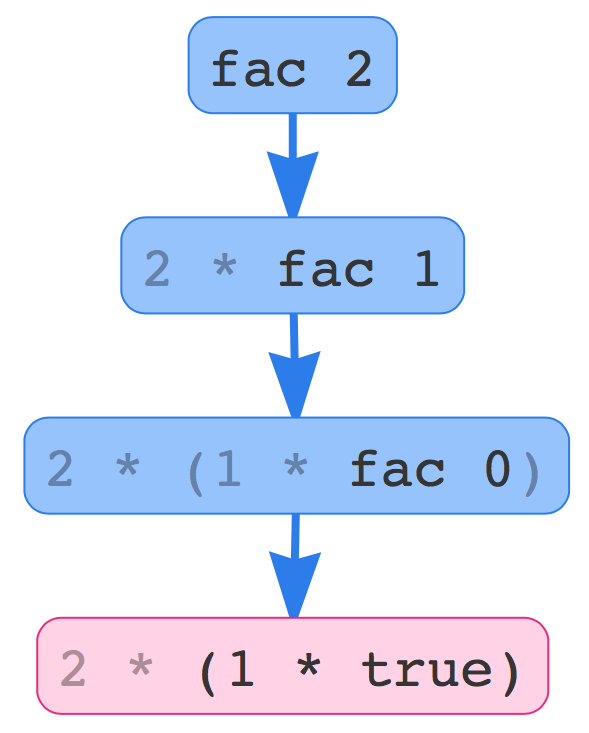
\includegraphics[height=2.5in]{fac-overview.png}
\end{minipage}
\caption{(L) An ill-typed \texttt{fac} function; (R) Dynamically witnessing the type error in \texttt{fac}}
\label{fig:factorial}
\end{figure}

In this paper we propose a new approach that explains 
static type errors by \emph{dynamically} witnessing
how exactly an ill-typed program goes wrong.
%
We have developed \toolname, an interactive tool that uses
the source of the ill-typed function to automatically synthesize
the result on the right in Figure~\ref{fig:factorial}, which
shows how the recursive calls reduce to a configuration where
the program ``goes wrong'' --- \ie\ the @int@ value @1@ is to be
multiplied with the @bool@ value @true@.
We achieve this via three concrete contributions.

\paragraph{1. Finding Witnesses}
Our first contribution is an algorithm for searching for
\emph{witnesses} to type errors, \ie\ inputs that cause a
program to go wrong~(\S~\ref{sec:semantics}).
%
This problem is surprisingly tricky when we cannot rely on
static type information.
%
In particular, we must avoid the trap of \emph{spurious} inputs
that cause irrelevant problems that would be avoided by picking
values of a different, relevant type.
%
We solve this problem by developing a novel operational semantics
that corresponds to executing the program with \emph{holes} ---
values whose type is unknown.
%
Our semantics \emph{conservatively} instantiates holes with concrete
values; thereby dynamically inferring the type of the input
until the program goes wrong.
%
We prove that our procedure synthesizes \emph{general witnesses},
which means, intuitively, that if a witness is found for a given
ill-typed function, then, \emph{for all} input types, there exist
inhabitants that can make the function go wrong.

Given a witness to a type error, the novice may still be at a loss.
%
The standard \ocaml\ interpreter and debugging infrastructure expect
well-typed programs, so they cannot be used to investigate \emph{how}
the witness causes the program to crash.
%
More importantly, the execution itself may be quite long and may contain
details not relevant to the actual error.

\paragraph{2. Visualizing Witnesses}
Our second contribution is a novel interactive visualization of the
execution of \ocaml\ programs, well-typed or not~(\S~\ref{sec:interactive}).
%
We extend the semantics to also build a \emph{reduction graph}
which records all of the small-step reductions and the context
in which they occur.
%
The graph lets us build a visualization that shows a sequence of
steps from the source witness to the stuck term and allows the user
to interactively expand the computation to expose intermediate steps,
by selecting an expression and choosing a traversal strategy.
%
The strategies include many of the standard debugging moves, \eg\
stepping \emph{forward} or \emph{into} or \emph{over} calls, as well
stepping or jumping \emph{backward} to understand how a particular
value was created, while preserving a context of the intermediate
steps that allow the user to keep track of a term's provenance.

\paragraph{3. Evaluating Witnesses}
%
Of course, the problem of finding witnesses is
undecidable. In fact, due to the necessarily
conservative nature of static typing, there
may not even exist any witnesses for a given
ill-typed program.
%
Thus, our approach is a heuristic that is only useful
if it can find \emph{compact} witnesses for
\emph{real-world} programs.
%
Our third contribution is an extensive evaluation of our approach
on two different sets of ill-typed programs obtained by instrumenting
compilers used in beginner's classes~(\S~\ref{sec:evaluation}).
%
The first is the \uwbench\ data set~\cite{lerner_searching_2007}
comprising \uwsize\ ill-typed programs.
%
The second is a new \ucsdbench\ data set, comprising \ucsdsize\
ill-typed programs.
%
We show that for both data sets, our technique is able to generate
witnesses for nearly 90\% of the programs, in under a second the
vast majority of cases.
%
Furthermore, we show that a simple interactive strategy yields
compact counterexample traces with fewer than 5 steps for 60\%
of the programs, and under 10 steps for 90\% of the programs.

\smallskip
Our results show that in the vast majority of
cases, (novices') ill-typed programs \emph{do} go wrong.
This, in turn, opens the door to a novel dynamic way to
explain, understand, and appreciate the benefits of static typing.

%%% Local Variables:
%%% mode: latex
%%% TeX-master: "main"
%%% End:

\section{Overview}
\label{sec:overview}

We start with an overview of our approach to
explaining (static) type errors using \emph{witnesses}
that (dynamically) show how the program goes wrong.
%
We illustrate why generating suitable inputs
to functions is tricky in the absence of type
information.
%
Then we describe our solution to the problem
and highlight the similarity to static type
inference,
%
Finally, we demonstrate our visualization of
the synthesized witnesses.

\subsection{Generating Witnesses}
\label{sec:generating-witnesses}
Our goal is to find concrete values
that demonstrate how a program ``goes wrong''.

\paragraph{Problem: Which inputs are bad?}
%
One approach is to randomly generate input values and
use them to execute the program until we find one that
causes the program to go wrong.
%
Unfortunately, this approach quickly runs aground.
Recall the erroneous @fac@ function from Figure~\ref{fig:factorial}.
%~\S~\ref{sec:introduction}:
%
% \begin{code}
  % let rec fac n =
    % if n <= 0 then
      % true
    % else
      % n * fac (n-1)
% \end{code}
% \ES{having two copies of \texttt{fac} seems silly, but the back-reference across a page boundary is no good either...}
%
What \emph{types} of inputs should we test @fac@ with?
%
Values of type @int@ are fair game, but values of type, say,
@string@ or @int list@ will cause the program to go wrong
in an \emph{irrelevant} manner.
%
Concretely, we want to avoid testing @fac@ with any type other
than @int@ because any other type would cause @fac@ to get stuck
immediately in the @n <= 0@ test.

\paragraph{Solution: Don't generate inputs until forced.}
Our solution is to avoid generating a concrete value for the input at
all, until we can be sure of its type.
%
The intuition is that we want to be as lenient as possible in our tests,
so we make no assumptions about types until it becomes clear from the
context what type an input must have.
%
This is actually quite similar in spirit to type inference.

To defer input generation, we borrow the notion of a ``hole'' from
SmallCheck~\cite{Runciman2008-ka}.
%
A hole --- written \vhole{\thole} --- is a \emph{placeholder} for a
value \ehole of some unknown type \thole.
%
We leave all inputs as uninstantiated holes until they are demanded by
the program, \eg due to a primitive operation like the @<=@ test.

\paragraph{Narrowing Input Types}
Primitive operations, data construction, and case-analysis \emph{narrow}
the types of values.
%
For concrete values this amounts to a runtime type check, we ensure that
the value has a type compatible with the expected type.
%
For holes, this means we now know the type it should
have (or in the case of compound data we know \emph{more} about the
type) so we can instantiate the hole with a value.
%
The value may itself contain more holes, corresponding to components
whose type we still do not know.
%
Consider the @fst@ function:
%
\begin{code}
  let fst p = match p with
    (a, b) -> a
\end{code}
%
The case analysis tells us that @p@ must be a pair, but it says
\emph{nothing} about the contents of the pair.
%
Thus, upon reaching the case-analysis we would generate a pair
containing fresh holes for the @fst@ and @snd@ component.
%
Notice the similarity between instantiation of type variables and
instantiation of holes.
%
We can compute an approximate type for @fst@ by approximating the types
of the (instantiated) input and output, which would give us:
%
\begin{mcode}
  fst : ($\thole_1$ * $\thole_2$) -> $\thole_1$
\end{mcode}
%
We call this type approximate because we only see a single path through
the program, and thus will miss narrowing points that only occur in
other paths.

Returning to @fac@, given a hole as input we will narrow the hole
to an @int@ upon reaching the @<=@ test.
%
At this point we choose a
random @int@\footnote{With standard heuristics~\cite{Claessen2000-lj} to favor small values.}
for the instantiation and
concrete execution takes over entirely, leading us to the expected crash
in the multiplication.

\paragraph{Witness Generality}
We show in \S~\ref{sec:soundness} that our lazy instantiation of holes
produces \emph{general witnesses}.
%
That is, we show that if ``executing''
a function with a hole as input causes the
function to ``go wrong'', then there is
\emph{no possible} type for the function.
%
In other words, for \emph{any} type you might
assign to the function, there exist inhabitants
that will cause the function to go wrong.

\paragraph{Problem: How many inputs does a function take?}
%
There is another wrinkle, though; how did we know
that @fac@ takes a single argument instead of two
(or none)?
%
It is clear, syntactically, that @fac@ takes \emph{at least} one
argument, but in a higher-order language with currying, syntax can be
deceiving.
%
Consider the following definition:
%
\begin{code}
  let incAllByOne = List.map (+ 1)
\end{code}
%
Is @incAllByOne@ a function?
%
If so, how many arguments does it take?
%
The \ocaml\ compiler deduces that @incAllByOne@ takes a single argument
because the \emph{type} of \hbox{@List.map@} says it takes two arguments, and it is
partially applied to @(+ 1)@.
%
As we are dealing with ill-typed programs we do not have the luxury of
typing information.

\paragraph{Solution: Search for saturated application.}
We solve this problem by deducing the number of arguments
via an iterative process. We add arguments one-by-one
until we reach a \emph{saturated} application, \ie\
until evaluating the application returns a value
other than a lambda.

\subsection{Visualizing Witnesses}
\label{sec:visual-witness}
We have described how to reliably find witnesses to type errors in \ocaml,
but this does not fully address our original goal --- to \emph{explain}
the errors.
%
Having identified an input vector that triggers a crash, a common next
step is to step through the program with a \emph{debugger} to observe
how the program evolves.
%
The existing debuggers and interpreters for \ocaml\ assume a type-correct
program, so unfortunately we cannot use them off-the-shelf.
%
Instead we extend our search for witnesses to produce an execution
trace.

\paragraph{Reduction Graph}
Our trace takes the form of a reduction graph, which records small-step
reductions in the context in which they occur.
%
% These graphs have two types of edges:
% %
% (1) ``steps-to'' edges that capture the small-step transition between
% two terms, and
% %
% (2) ``sub-term'' edges that capture the containment relation between two
% terms.
%
For example, evaluating the expression @1+2+3@ would produce the
graph in Figure~\ref{fig:simple-reduction-hi}.
%
\begin{figure}[t]
  \centering
  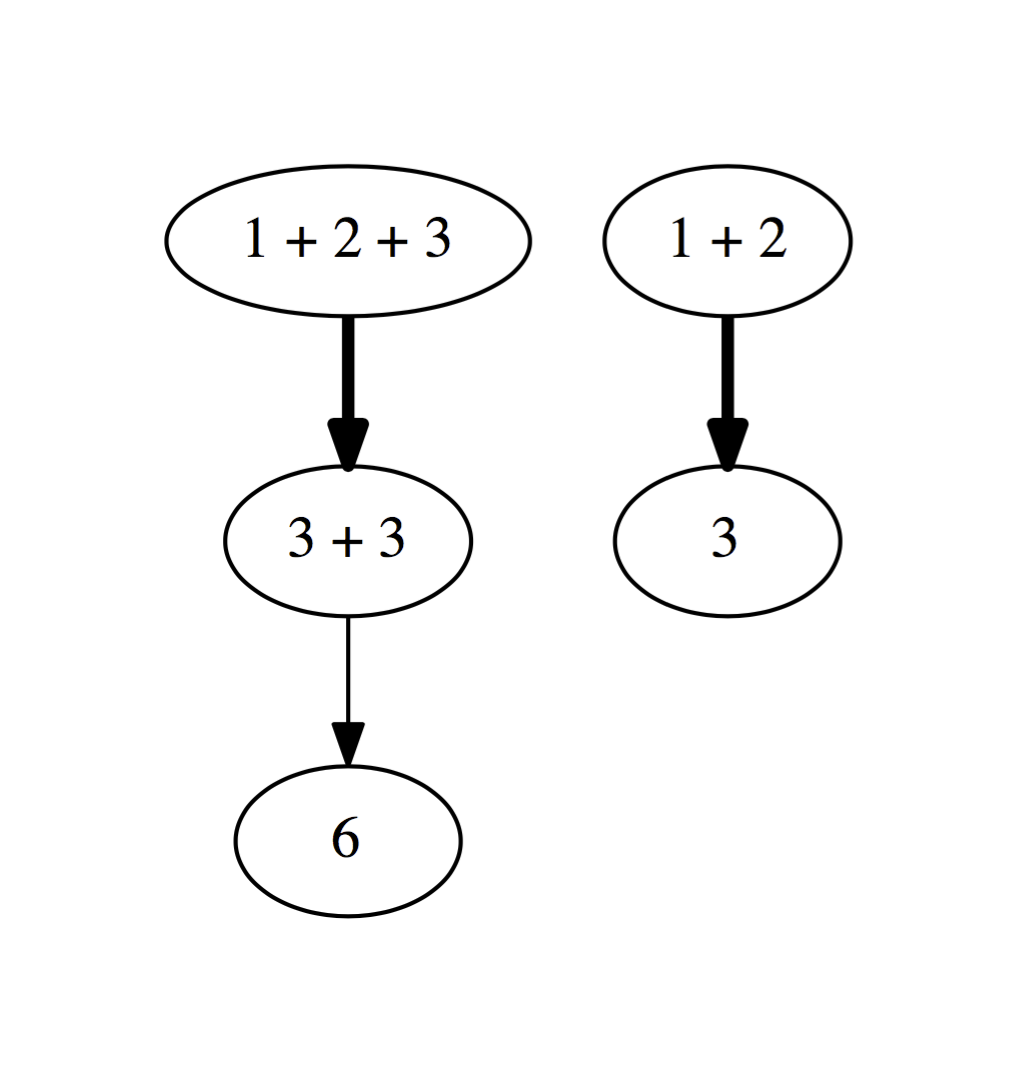
\includegraphics[height=2in]{simple.png}
  \caption{The reduction graph for \texttt{1+2+3}. The two edges
    produced by the transition from \texttt{1+2+3} to \hbox{\texttt{3+3}}
    are highlighted.}
\label{fig:simple-reduction-hi}
\end{figure}
%
Notice that when we transition from @1+2+3@ to @3+3@ we collect
both that edge \emph{and} an edge from the sub-term @1+2@ to @3@.
%
These additional edges allow us to implement two common debugging
operations \emph{post-hoc}: ``step into'' to zoom in on a specific
function call, and ``step over'' to skip over an uninteresting
sub-computation.

\paragraph{Interacting with the graph}
The reduction graph is useful for formulating and executing traversals,
but displaying it all at once would quickly become overwhelming.
%
Our interaction begins by displaying a big-step reduction, \ie the
witness followed by the stuck term.
%
The user can then progressively fill in the hidden steps of the
computation by selecting a visible term and choosing one of the
applicable traversal strategies --- described in
\S~\ref{sec:interactive} --- to insert another term into the
visualization.

\paragraph{Jump-compressed Witnesses}
It is rare for the initial state of the visualization to be
informative enough to diagnose the error.
%
Rather than abandon the user, we provide a short-cut to expand the witness
to a \emph{jump-compressed} trace, which contains every function call
and return step.
%
The jump-compressed trace abstracts the computation as a sequence of
call-response pairs, providing a high-level overview of steps taken
to reach the crash, and a high level of compression compared to the
full trace.
%
For example, the jump-compressed trace in Figure~\ref{fig:factorial}
contains 4 nodes compared to the 19 in the fully expanded trace.
%
Our benchmark suite of student programs shows that jump-compression is
practical, with an average jump-compressed trace size of 7 nodes and a
median of 5.

% A sample interaction with the trace of @fac 1@ can be seen in
% Figure~\ref{fig:nanomaly-factorial}.
% %
% % \begin{figure*}[t]
% % \centering
% % 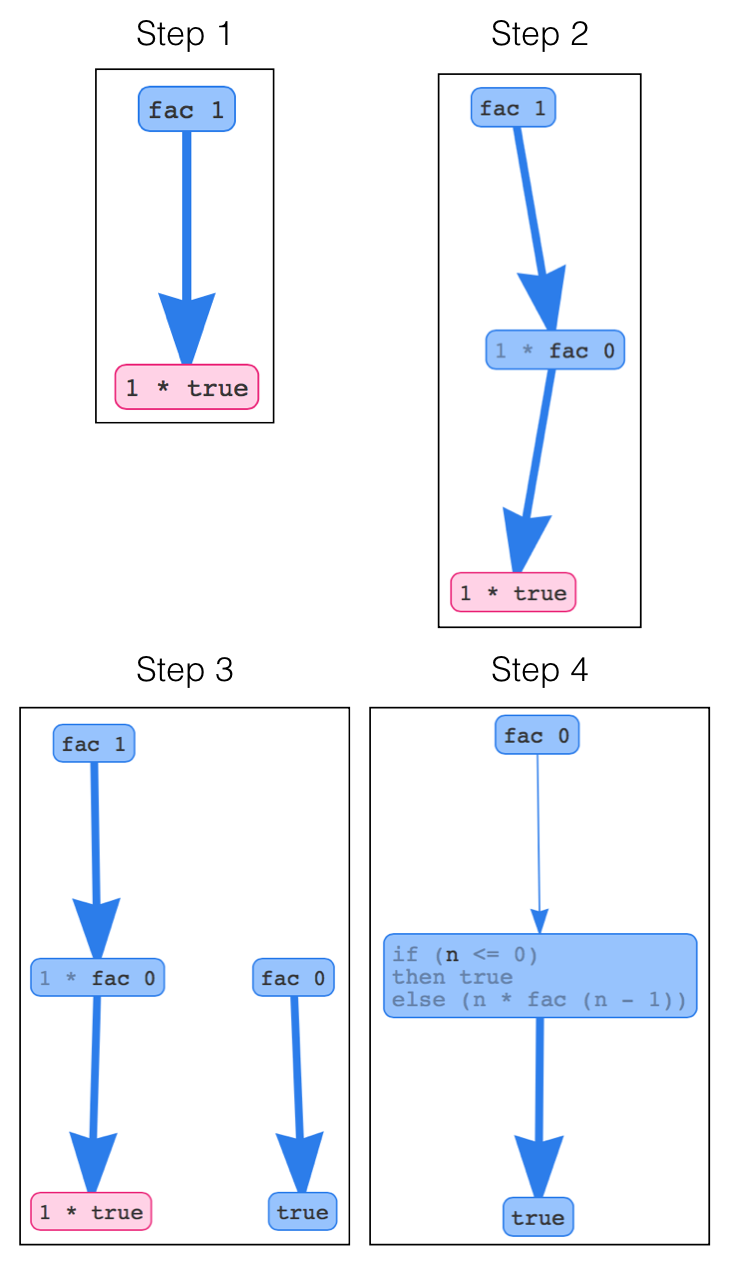
\includegraphics[width=0.8\linewidth]{fac-steps.png}
% % \caption{A sequence of interactions with the trace of
% %   \texttt{fac 1}. The stuck term is red, in each node the redex is
% %   highlighted. Thick arrows denote a multi-step transition, thin arrows
% %   denote a single-step transition. We start in step 1. In step 2 we jump
% %   forward from the witness to the next function call. In step 3 we step
% %   into the recursive \texttt{fac 0} call, which spawns a new ``thread''
% %   of execution. In step 4 we take a single step forward from
% %   \texttt{fac 0} (hiding the context for space).}
% % \label{fig:nanomaly-factorial}
% % \end{figure*}
% %
% The initial state of the visualization tells us that after some number
% of steps -- the thick arrow denotes a multi-step transition -- we try to
% multiply @1@ by @true@.

% Upon seeing the stuck term, we might wonder where @true@ came from.
% %
% To investigate we select the stuck term and click the ``jump backward''
% button to search backwards from the stuck term for the most recent
% function call, which brings us to @1 * fac 0@. Notice at this point that
% @fac 0@ is highlighted while @1 *@ is grayed out. This tells us that
% @fac 0@ is the redex in this term.

% @fac 0@ seems like the right thing to do so we choose to ``step into''
% it, which inserts a new multi-step transition from @fac 0@ to @true@.
% %
% Finally, we take a ``step forward'' from \hbox{@fac 0@,} bringing us to @fac@'s
% body. If we mouse over the body term we will see a popup with the
% environment at this point, notably telling us that @n = 0@. At this point
% it is clear that @fac@ handles the @n <= 0@ case incorrectly and should
% instead return an @int@.

% Upon seeing the stuck term, one might wonder where the @function@
% came from.
% %
% To investigate we select the stuck term and click the ``jump backward''
% button to search backwards from the stuck term for the most recent
% function call, which brings us to @listReverse [] = w@, in the same
% context as before.
% %
% Uncontent with the explanation so far, we ``step forward'' twice from
% the @listReverse []@ term, bringing us to @helper [] = w@.
% %
% At this point it is clear that the @helper@ function is not defined
% correctly, we have supplied it with the single argument we expected and
% yet it still returned a @function@.

% The problem is that the @function@ keyword in \ocaml defines an
% anonymous function that takes a single argument and immediately does a
% case-analysis without giving the argument a name.
% %
% The solution is to replace @function@ with an explicit @match xs with@
% -- naming the value we wish to case-analyse.
% %
% After applying our fix, \nanomaly -- and more importantly \ocaml --
% decide that @listReverse@ is safe to run.
% \ES{these last few paragraphs probably belong in the overview}
%





%%% Local Variables:
%%% mode: latex
%%% TeX-master: "main"
%%% End:

\section{Type-Error Witnesses}
\label{sec:searching-witness}

% Our goal is to find concrete values that demonstrate how a
% program ``goes wrong''.

% \paragraph{Problem: Which inputs are bad?}
% %
% One approach is to randomly generate input values and use
% them to execute the program until we find one that causes
% the program to go wrong. However, to see why this approach
% is naive, consider the following example:
% %
% \begin{lstlisting}
%   let f x =
%     let y = 1 + x in
%       1. +. y
% \end{lstlisting}
% %
% What \emph{types} of inputs should we test \texttt{f} with?
% Values of type \texttt{int} and \texttt{float} are fair game,
% but values of type say, \texttt{string} or \texttt{int list}
% will cause the program to go wrong in an \emph{irrelevant}
% manner.

% \paragraph{Solution:} \RJ{STOP}


% we cannot provide \emph{completely arbitrary} inputs to
% \texttt{f}. Instead, we call \texttt{f} with a \emph{hole}, written
% \ehole{}, which is a placeholder for a value whose type we have not
% yet determined. As we execute the program, we instantiate holes with
% concrete values as demanded by the primitive operations in the
% program. For example, the hole we pass to f will be instantiated to an
% int when we reach the \lstinline{1 + x} term. Thus, y will be an int as
% well, and the program will get stuck at \lstinline{1. +. y}. \ES{this
%   reads more like overview text..}
%


% \begin{itemize}
% \item how do we run ill-typed programs?
% \item for a lang like ocaml, dynamic semantics are independent of static
%   semantics, just lambda calculus. so no problem to run ill-typed
%   program
% \item but what about functions? what type of arguments should we pass? consider
%
% \begin{lstlisting}
% let f x =
%   let y = 1 + x in
%     1. +. y
% \end{lstlisting}
%
% does \texttt{f} take an int, float, string? int and float are both
% somewhat plausible, but string or anything else is ``clearly'' bogus. so
% we cannot provide \emph{completely arbitrary} inputs to
% \texttt{f}. Instead, we call \texttt{f} with a \emph{hole}, written
% \ehole{}, which is a placeholder for a value whose type we have not
% yet determined. As we execute the program, we instantiate holes with
% concrete values as demanded by the primitive operations in the
% program. For example, the hole we pass to f will be instantiated to an
% int when we reach the \lstinline{1 + x} term. Thus, y will be an int as
% well, and the program will get stuck at \lstinline{1. +. y}. \ES{this
%   reads more like overview text..}
%
% % \item values are tagged with their types, just like ``untyped'' langs
% % \item special ``hole'' value whose type is not yet known, used for function args
% % \item on-the-fly unification to determine ``correct'' type for holes
% \end{itemize}


Next, we formalize the notion of type error witnesses as follows.
%
First, we define a core calculus within which we will work~\S~\ref{sec:syntax}.
%
Second, we develop a (non-deterministic) operational semantics
for ill-typed programs that precisely defines the notion
of a \emph{witness}~\S~\ref{sec:semantics},
%
Third, we formalize and prove a notion of \emph{generality} for
witnesses, which states, intuitively that if we find a
single witness then for \emph{every possible} type
assignment, there exist inputs that are guaranteed to make
the program ``go wrong''~\S~\ref{sec:soundness}, and finally,
%
Fourth, we refine the operational semantics into a
\emph{search procedure} that returns concrete (general)
witnesses for ill-typed programs~\S~\ref{sec:search-algorithm}.

\subsection{Syntax}
\label{sec:syntax}
\begin{figure}
% \hrule width 0.48\textwidth \vspace{0.05in}
$$
\begin{array}{rrcl}
% \emphbf{Configurations} \quad
%   & c & ::=    & \triple{e}{\vsu}{\tsu} \spmid \triple{\stuck}{\vsu}{\tsu} \\[0.05in]

\emphbf{Expressions}
  & \estuck & ::= & e \spmid \stuck \\
  & e & ::=    & v \spmid x \spmid \eapp{e}{e} \spmid \eplus{e}{e}\\
  &   & \spmid & \eif{e}{e}{e} \\
  % &   & \spmid & \elet{x}{e}{e} \\
  &   & \spmid & \epair{e}{e} \spmid \epcase{e}{x}{x}{e} \\
  &   & \spmid & \enode{e}{e}{e} \spmid \eleaf \\
  &   & \spmid & \ecase{e}{e}{x}{x}{x}{e} \\[0.1in]

\emphbf{Values}
  & v  & ::= & n \spmid b \spmid \efun{x}{e} \spmid \vhole{\thole} \spmid tr \\
  & tr & ::= & \vnode{t}{v}{v}{v} \spmid \vleaf{t} \\[0.05in]

\emphbf{Integers}
  & n & ::= &  0,1,-1,\ldots \\[0.05in]

\emphbf{Booleans}
  & b & ::= &  \etrue \spmid \efalse \\[0.05in]

\emphbf{Types}
  & t & ::=     & \tbool \spmid \tint \spmid \tfun \\
  &   &  \spmid & \tprod{t}{t} \spmid \ttree{t} \spmid \thole \\[0.05in]

\emphbf{Substitutions}
  & \vsu & ::= & \emptysu \spmid \extendsu{\vsu}{\vhole{\thole}}{v} \\
  & \tsu & ::= & \emptysu \spmid \extendsu{\tsu}{\thole}{t} \\[0.1in]
% \end{array}
% $$
% % \hrule width 0.48\textwidth
% $$
% \begin{array}{rrcl}
\emphbf{Contexts}
  & C
  & ::=
  &   	 \bullet
  \spmid \eapp{C}{e}
  \spmid \eapp{v}{C} \\
  & & \spmid & \eplus{C}{e} \spmid \eplus{v}{C} \\
  & & \spmid & \eif{C}{e}{e} \\
  % & & \spmid & \elet{x}{C}{e} \\
  & & \spmid & \epair{C}{e} \spmid \epair{v}{C} \\
  & & \spmid & \epcase{C}{x}{x}{e} \\
  & & \spmid & \enode{C}{e}{e} \\
  & & \spmid & \enode{v}{C}{e} \\
  & & \spmid & \enode{v}{v}{C} \\
  & & \spmid & \ecase{C}{e}{x}{x}{x}{e} \\[0.05in]

\emphbf{Type Contexts}
  & T &::=& \bullet \spmid \ttree{T} \spmid \tprod{T}{t} \spmid \tprod{t}{T} \\[0.05in]
\end{array}
$$

% \judgementHead{Reduction}{\eval{e}{e}}

% $$
% \begin{array}{rcl}
% \eval{C[e]&}{&C[e']} \qquad \text{if}\ \eval{e}{e'} \\
% 	\eval{\eapp{c}{v}&}{& \ceval{c}{v}}\\
% \eval{\eapp{(\efun{x}{\tau_x}{e})}{e_x}&}{&e\sub{x}{e_x}}\\
% 	\eval{\elet{x}{e_x}{e}&}{&e\sub{x}{e_x}} \\
% 	\eval{\ecase{D_j\ \overline{e}}{D_i}{\overline{y_i}}{e_i}{x}&}
% 	{&e_j\sub{x}{D_j\ \overline{e}}\sub{\overline{y_j}}{\overline{e}}} \\
% \end{array}
% $$

\caption{Syntax of \lang}
\label{fig:syntax}
\end{figure}

%
Figure~\ref{fig:syntax} describes the syntax of \lang, a simple lambda
calculus with integers, booleans, and binary trees.
%
As we are specifically interested in programs that \emph{do} go wrong,
we include an explicit \stuck\ state in our syntax.

\paragraph{Holes}
\label{sec:holes}
%
Recall that a key challenge in our setting is to find witnesses
that are meaningful and do not arise from choosing values from
irrelevant types.
%
We solve this problem be equipping our term language with a
notion of a \emph{hole}, written \vhole{\thole}, which represents
an \emph{unconstrained} value $\ehole$ that may be replaced with
\emph{any} value of type \thole.
%
Intuitively, the type holes \thole\ can be viewed as type variables
that we will \emph{not} generalize over.
%
A \emph{normalized} value (resp.\ type) is one that is not a hole,
but which may internally contain holes.
%
For example \RJ{add example here}

\paragraph{Substitutions}
%
Our semantics ensure the generality of witnesses by incrementally
\emph{refining} holes, filling in just as much information as is
needed locally to make progress (inspired by the manner in
which SmallCheck uses lazy evaluation~\cite{runciman_smallcheck_2008}).
%
We track how the holes are incrementally filled in, by using
value (resp.\ type) \emph{substitutions} $\vsu$ (resp. $\tsu$)
that map value (resp.\ type) holes to values (resp.\ types).
%
A \emph{normalized} substitution is one whose co-domain comprises
of normalized values (resp.\ types).
%
In the sequel, we will assume and ensure that all substitutions
are normalized.

\paragraph{Resolving Holes}
We \emph{resolve} a hole with respect to a substitution by
transitively applying the substitution as long as it contains
any holes that are defined in the substitution.
%
We write \resolve{\thole}{\tsu} to denote the the resolution
of \thole\ with respect to \tsu.
%
Note that by definition, \resolve{\thole}{\tsu} does not contain
any holes in the domain of \tsu.


\subsection{Semantics}
\label{sec:semantics}
%
\RJ{Add intuition text -- "dynamic Hindley Milner"}
%
The substitutions let us ensure that we consistently instantiate
each hole with the same (partially defined) value or type, regardless
of the multiple contexts in which the hole appears. This ensures we
can report a concrete (and general) witness for any (dynamically)
discovered type errors.

The evaluation relation is parameterized by a pair of functions:
called \emph{narrow} (\forcesym) and \emph{generate} (\gensym),
that ``dynamically'' perform type-checking and hole-filling
respectively.

\paragraph{Narrowing Types} The procedure % $\force{v}{t}{\vsu}{\tsu}$,
$$
\forcesym :: (v, t, \vsu, \tsu) \rightarrow \triple{v \cup \stuck}{\vsu}{\tsu}
$$
defined in Figure~\ref{fig:narrow}, takes as input a value $v$, a type
$t$, and the current value and type substitutions, and refines $v$ to
have type $t$ by yielding a triple of either the same value and
substitutions, or yields the stuck state if no such refinement is
possible. In the case where $v$ is a hole, it first checks in the given
$\vsu$ to see if the hole has already been instantiated and, if so,
returns the existing instantiation.
%
\begin{figure*}[ht]
$$
\begin{array}{lcl}
%% \multicolumn{3}{l}{\forcesym \ :: \  (e, t) \rightarrow \pair{e}{\vsu}} \\
\forcesym                  & ::     & (v, t, \vsu, \tsu) \rightarrow \triple{v \cup \stuck}{\vsu}{\tsu} \\
% \force{v}{\thole}{\vsu}{\tsu}  & \defeq & \hspace{-1ex}
% \begin{cases}
%   \triple{v}{\vsu}{\tsu'} & \mbox{if } \tsu' = \unify{\{\typeof{v}, \thole\}}{\tsu} \\
%   \triple{\stuck}{\vsu}{\tsu} & \mbox{otherwise} \\

%   % \force{v}{\subst{\tsu}{\thole}}{\vsu}{\tsu} & \mbox{if}\ \thole \in dom(\tsu) \\
%   % \triple{v}{\vsu}{\extendsu{\tsu}{\thole}{\typeof{v}}} & \mbox{otherwise} \\
% \end{cases} \\
\force{\vhole{\thole}}{t}{\vsu}{\tsu} & \defeq & \hspace{-1ex}
\begin{cases}
  \triple{v}{\vsu}{\tsu'}    & \mbox{if } v = \lookupsu{\vsu}{\ehole},
                                         \tsu' = \unify{\{\thole, t, \typeof{v}\}}{\tsu}\\
  \triple{\stuck}{\vsu}{\tsu} & \mbox{if } v = \lookupsu{\vsu}{\ehole} \\
  \triple{v}{\extendsu{\vsu}{\ehole}{v}}{\tsu'} & \mbox{if}\ \tsu' = \unify{\{\thole, t\}}{\tsu}, v = \gen{t_1}{\tsu'}\\
\end{cases} \\
% \begin{cases}
%   \triple{\lookupsu{\vsu}{\ehole}}{\vsu}{\tsu} & \mbox{if}\ \ehole \in dom(\vsu), \hastype{\lookupsu{\vsu}{\ehole}}{t} \\
%   \triple{\stuck}{\vsu}{\tsu}                  & \mbox{if}\ \ehole \in dom(\vsu) \\
%   \triple{v}{\extendsu{\vsu}{\ehole}{v}}{\tsu}   & v = \gen{t}\\
% \end{cases} \\
 % \begin{array}{l}
    % \mathtt{if}\ i \in \vsu\ \mathtt{then}\ \triple{\vsu(i)}{\vsu}\ \mathtt{else} \\
         % \elet{v}{\gen{t}}{\triple{v}{\ehole{i} \mapsto v}}
  % \end{array} \\
\force{n}{\tint}{\vsu}{\tsu}     & \defeq & \triple{n}{\vsu}{\tsu} \\
\force{b}{\tbool}{\vsu}{\tsu}    & \defeq & \triple{b}{\vsu}{\tsu} \\
\force{\efun{x}{e}}{\tfun}{\vsu}{\tsu} & \defeq & \triple{\efun{x}{e}}{\vsu}{\tsu} \\
\force{\vleaf{t_1}}{\ttree{t_2}}{\vsu}{\tsu} & \defeq & \triple{\vleaf{t_1}}{\vsu}{\tsu'}, \mbox{if}\ \tsu' = \unify{\{t_1, t_2\}}{\tsu} \\
\force{\vnode{t_1}{v_1}{v_2}{v_3}}{\ttree{t_2}}{\vsu}{\tsu} & \defeq & \triple{\vnode{t_1}{v_1}{v_2}{v_3}}{\vsu}{\tsu'}, \mbox{if}\ \tsu' = \unify{\{t_1, t_2\}}{\tsu} \\
\force{v}{t}{\vsu}{\tsu} & \defeq & \triple{\stuck}{\vsu}{\tsu}
\end{array}
$$
\caption{Narrowing values}
\label{fig:narrow}
\end{figure*}
%
%While a hole may map to a value that \emph{contains} another hole, \eg a
%lambda or a tree, it may not map \emph{directly} to another hole,
As the substitutions are normalized, in the first case of \forcesym\ we
do not need to \forcesym\ the result of the substitution, the sub-hole
will be narrowed when the context demands it.

\paragraph{Generating Values} The (non-deterministic)
$\gen{t}{\tsu}$ in Figure~\ref{fig:gen}, takes
as input a type $t$ and returns a value of that type.
%
For base types, the procedure returns an arbitrary value of
that type.
%
For functions, it returns a lambda with a \emph{new} hole
denoting the return value, and unconstrained types (denoted
by $\thole$) yield fresh holes constrained to have type
\thole (denoted by $\vhole{\thole}$).
%
Note that for an algebraic datatype, $\gen{\ttree{t}}{\tsu}$
will always place holes in the generated nodes; they will be
lazily filled in later, on demand.


\begin{figure}[ht]
$$
\begin{array}{lcll}
\gensym       & ::  & (t, \tsu) \rightarrow v \\
\gen{\thole}{\tsu}  & \defeq  & \gen{\subst{\tsu}{\thole}}{\tsu}, & \quad \text{if } \thole \in dom(\tsu) \\
\gen{\tint}{\tsu}   & \defeq  & n, & \quad \text{non-deterministic} \\
\gen{\tbool}{\tsu}  & \defeq  & b, & \quad \text{non-deterministic} \\
\gen{\ttree{t}}{\tsu}  & \defeq  & tr, & \quad \text{non-deterministic} \\
\gen{\tfun}{\tsu}   & \defeq & \efun{x}{\vhole{\thole}}, & \quad \text{\ehole and \thole are fresh} \\
\gen{\thole}{\tsu}  & \defeq & \vhole{\thole}, & \quad \text{\ehole is fresh} \\
\end{array}
$$
\caption{Generating values}
\label{fig:gen}
\end{figure}


\paragraph{Steps and Traces}
\begin{figure*}
\judgementHead{Evaluation}{\step{e}{\su}{e}{\su}}
\begin{gather*}
\inference[\recontext]
  {\step{e}{\su}{e_1}{\su_1}}
  {\step{C[e]}{\su}{C[e_1]}{\su_1}}
\qquad
\inference[\restuck]
  {}
  {\step{C[\stuck]}{\su}{\stuck}{\su}}
\\ \\
\inference[\replusgood]
  {\pair{n_1}{\su_2} = \force{v_1}{\tint} \\
   \pair{n_2}{\su_3} = \force{v_2}{\tint} \\ 
   n = \eplus{n_1}{n_2}}
  {\step{\eplus{v_1}{v_2}}{\su_1}{n}{\su_1;\su_2;\su_3}}
\qquad
\inference[\replusbadone]
  {\pair{\stuck}{\su_2} = \force{v_1}{\tint}}
  {\step{\eplus{v_1}{v_2}}{\su_1}{\stuck}{\su_1;\su_2}}
\\ \\
\inference[\replusbadtwo]
  {\pair{\stuck}{\su_2} = \force{v_2}{\tint}}
  {\step{\eplus{v_1}{v_2}}{\su_1}{\stuck}{\su_1;\su_2}}
\qquad
\inference[\reifgoodone]
  {\pair{\etrue}{\su_2} = \force{v}{\tbool}}
  {\step{\eif{v}{e_1}{e_2}}{\su_1}{e_1}{\su_1;\su_2}}
\\ \\
\inference[\reifgoodtwo]
  {\pair{\efalse}{\su_2} = \force{v}{\tbool}}
  {\step{\eif{v}{e_1}{e_2}}{\su_1}{e_2}{\su_1;\su_2}}
\qquad
\inference[\reifbad]
  {\pair{\stuck}{\su_2} = \force{v}{\tbool}}
  {\step{\eif{v}{e_1}{e_2}}{\su_1}{\stuck}{\su_1;\su_2}}
\\ \\
\inference[\reappgood]
  {\pair{\efun{x}{e}}{\su_2} = \force{v_1}{\tfun{\thole{}}{\thole{}}}}
  {\step{\eapp{v_1}{v_2}}{\su_1}{e\sub{x}{v_2}}{\su_1;\su_2}}
\qquad
\inference[\reappbad]
  {\pair{\stuck}{\su_2} = \force{v_1}{\tfun{\thole{}}{\thole{}}}}
  {\step{\eapp{v_1}{v_2}}{\su_1}{\stuck}{\su_1;\su_2}}
\\ \\
\inference[\relet]
  {}
  {\step{\elet{x}{v}{e}}{\su}{e\sub{x}{v}}{\su}}
\end{gather*}
\\ % [0.05in]
\relDescription{\forcesym and \gensym}
\begin{gather*}
\begin{array}{lcl}
\force{\ehole{i}}{t} & \defeq & \elet{v}{\gen{t}}{\pair{v}{\ehole{i} \mapsto v}} \\
\force{v}{\ehole{}}  & \defeq & \pair{v}{\emptysu} \\
\force{n}{\tint}    & \defeq & \pair{n}{\emptysu} \\
\force{v}{\tint}    & \defeq & \pair{\stuck}{\emptysu} \\
\force{b}{\tbool}   & \defeq & \pair{b}{\emptysu} \\
\force{v}{\tbool}   & \defeq & \pair{\stuck}{\emptysu} \\
\force{\efun{x}{e}}{\tfun{\thole{}}{\thole{}}} & \defeq & \pair{\efun{x}{e}}{\emptysu} \\
\force{v}{\tfun{\thole{}}{\thole{}}} & \defeq & \pair{\stuck}{\emptysu} \\
\end{array}
\qquad
\begin{array}{lcll}
\gen{\tint}   & \defeq & n & \\
\gen{\tbool}  & \defeq & b & \\
\gen{\tfun{t_1}{t_2}} & \defeq & \efun{x}{\ehole{i}}, & \quad \text{$i$ is fresh} \\
\gen{\thole{}} & \defeq & \ehole{i}, & \quad \text{$i$ is fresh} \\
\end{array}
\end{gather*}
\caption{Evaluation relation}
\label{fig:operational}
\end{figure*}

%
% WRW notes that Figure 4 does not seem to handle recursion (it's not clear
% how the let rule would work for something "let rec"-y, and there's not
% function call rule). I only mention this because I can imagine a reviewer
% wondering about your ability to generate good witnesses for function
% types. This could likely be addressed in text, by a forward reference to
% Section 3.4 where higher-order functions are handled, without changing
% any of the formalisms at the last minute.
Figure~\ref{fig:operational} describes the small-step contextual
reduction semantics for \lang.
%
A program state is a triple $\triple{e \cup \stuck}{\vsu}{\tsu}$ of an
expression $e$ or the stuck term $\stuck$, a value substitution $\vsu$,
and a type substitution $\tsu$. In the sequel we will write \estuck to
denote either an expression $e$ or \stuck.
%
We write $\step{\estuck}{\vsu}{\tsu}{\estuck'}{\vsu'}{\tsu'}$ if the state
$\triple{\estuck}{\vsu}{\tsu}$ transitions in a \emph{single step} to
$\triple{\estuck'}{\vsu'}{\tsu'}$.
%
A (finite) \emph{trace} $\trace$ is a sequence of configurations
$\triple{\estuck_0}{\vsu_0}{\tsu_0}, \ldots, \triple{\estuck_n}{\vsu_n}{\tsu_n}$ such that
$\forall 0 \leq i < n$, we have
$\step{\estuck_i}{\vsu_i}{\tsu_i}{\estuck_{i+1}}{\vsu_{i+1}}{\tsu_{i+1}}$.
%
We write \steptr{\trace}{\estuck}{\vsu}{\tsu}{\estuck'}{\vsu'}{\tsu'} if $\trace$ is
a trace of the form $\triple{\estuck}{\vsu}{\tsu},\ldots,\triple{\estuck'}{\vsu'}{\tsu'}$.
%
We write \steps{\estuck}{\vsu}{\tsu}{\estuck'}{\vsu'}{\tsu'} if
\steptr{\trace}{\estuck}{\vsu}{\tsu}{\estuck'}{\vsu'}{\tsu'} for some trace $\trace$.

\paragraph{Primitive Reductions}
%
\RJ{Put high-level intuition about how "dynamic HM" is
formalized in op-sem, to set up next few paragraphs}
%
Primitive reduction steps --- addition, if-elimination,
function application, and data construction and case
analysis --- use \forcesym to ensure that values have
the appropriate type (and that holes are instantiated)
before continuing the computation.
%
Importantly, beta-reduction \emph{does not} type-check its
argument, it only ensures that ``the caller'' $v_1$ is indeed
a function.

\paragraph{Recursion}
\RJ{this para appears out of nowhere --- non-sequitur}
Fixed-point operators often cannot be typed in static type
systems, but we are not concerned with \emph{assigning}
types to terms, rather with showing that \emph{no type}
can be assigned.
%
We are simply executing the untyped $\lambda$-calculus,
which has no issue handling recursion.

%% \begin{thm}
%% \label{thm:all-reduce}
%%   Every closed expression $e$ reduces to a value $v$ (which may be \stuck).
%% \ES{do we really need to state this, or is it obvious?}
%% \end{thm}

% \begin{proof}%[Proof of \autoref{thm:all-reduce}]
%   Simple induction on the evaluation relation.
% \end{proof}

\subsection{Generality}\label{sec:soundness}

A key technical challenge in generating witnesses is
that we have no (static) type information to rely upon.
%
Thus, we must avoid the trap of generating \emph{spurious}
witnesses that arise from picking irrelevant values, when
instead there exist perfectly good values of a \emph{different}
type, under which the program would not have gone wrong.
%
We now show that our evaluation relation instantiates holes
in a \emph{general} manner. That is, given a function $f$,
if we have $\steps{\eapp{f}{\vhole{\thole}}}{\emptysu}{\emptysu}{\stuck}{\vsu}{\tsu}$,
then \emph{for every} input type $t$, we can find a value
$v$ of type $t$ such that $\eapp{f}{v}$ goes wrong.

\begin{thm}{\textbf{[Witness Generality]}}
\label{thm:soundness}
  For any function $f$, if\\
  \hbox{$\steptr{\trace}{\eapp{f}{\vhole{\thole}}}{\emptysu}{\emptysu}{\stuck}{\vsu}{\tsu}$,}
  then for every % inhabitable
  type
  % \footnote{We exclude builtin functions that subvert the type system, \eg \texttt{Obj.magic}, and thus consider the type $\forall a b. \tfun{a}{b}$ to be uninhabitable.}
  $t$ there exists a $v$ of type $t$ such that
  $\steps{\eapp{f}{v}}{\emptysu}{\emptysu}{\stuck}{\vsu}{\tsu}$.
\end{thm}

We need to develop some machinery in order to prove this theorem.
First, we show how our evaluation rules encode a dynamic form of
type inference, and next, we show that the types inferred via
evaluation are indeed maximally general.

\paragraph{The Type of a a Value} The \emph{dynamic type}
of a value $v$ is defined as a function $\typeof{v}$ shown
in Figure~\ref{fig:typeof}.
%
The types of primitive values are defined in the natural manner.
%
The types of functions are \emph{approximated}, which is all
that is needed to ensure an application does not get stuck, \eg
$$\typeof{\efun{x}{\eplus{x}{1}}} = \tfun$$
instead of $\tint \rightarrow \tint$.
%
The types of (polymorphic) data types are obtained from the
labels on their values.

\begin{figure}[ht]
\[ \begin{array}{lcll}
    \typeof{n}   & \defeq & \tint & \\
    \typeof{b}   & \defeq & \tbool & \\
    \typeof{\efun{x}{e}} & \defeq & \tfun \\
    \typeof{\vleaf{t}} & \defeq & \ttree{t} \\
    \typeof{\vnode{t}{v_1}{v_2}{v_3}} & \defeq & \ttree{t} \\
    \typeof{\vhole{\thole}} & \defeq & \thole \\
    % \typeof{\eleaf} & \defeq & \ttree{\thole}, & \quad \text{\thole is fresh} \\
    % \typeof{\enode{v_1}{v_2}{v_3}} & \defeq & \ttree{\thole}, & \quad \text{\thole is fresh} \\
    % \typeof{e} & \defeq & \thole, & \quad \text{\thole is fresh} \\
  \end{array} \]
\caption{The \emph{dynamic type} of a value.}
\label{fig:typeof}
\end{figure}

\paragraph{Dynamic Type Inference}
We can think of the evaluation of \eapp{f}{\vhole{\thole}}
as synthesizing a partial instantiation of \thole, and hence,
\emph{dynamically inferring} a (partial) type for $f$'s input.
%
We can extract this type from an evaluation trace, by
\emph{resolving} the \thole\ with the final type
substitution at the end of the trace.
%
Formally, we say that if
$\steptr{\trace}{\eapp{f}{\vhole{\thole}}}{\emptysu}{\emptysu}{\estuck}{\vsu}{\tsu}$,
then the \emph{partial input type} of $f$ upto $\trace$, written
\ptype{\trace}{f}, is $\resolve{\thole}{\tsu}$.

%repeatedly
%applying the final type substitution to \thole until it contains no
%holes in the domain of the substitution. We will call this process of
%repeated substition \emph{resolving} a hole, and will use
%\resolve{\thole}{\tsu} to denote the the resolution of \thole with
%respect to \tsu.



%$\typeof{\subst{\vsu}{\ehole}}$.
% \ES{should we say $\subst{\tsu}{\thole}$ instead? would need a helper function that does the repeated application of \tsu\ until the result has no $\thole \in dom(\tsu)$}
%
%We will omit the subscript when we wish to refer to the final partial
%type, \ie\ at the step where the expression has been reduced to a value
%(or stuck.)

% \begin{lem}
% \label{lem:narrow-tsu}
% If $\trace \defeq \triple{\eapp{f}{\vhole{\thole}}}{\emptysu}{\emptysu},\ldots$
% and $\trace' \defeq \trace, \triple{\estuck'}{\vsu'}{\tsu'}$
%     (\ie $\trace'$ is a single-step extension of $\trace$)
% and $\tsu \neq \tsu'$
% then the final step must have \emph{successfully} invoked \forcesym.
% \end{lem}

\paragraph{Narrowing}
%
Only a successful call to \forcesym can change the partial
input type of $f$.
%
\begin{lem}
\label{lem:force-inst}
If
$\trace \defeq \triple{\eapp{f}{\vhole{\thole}}}{\emptysu}{\emptysu},\ldots,\triple{e}{\vsu}{\tsu}$
and
$\trace' \defeq \trace, \step{e}{\vsu}{\tsu}{\estuck'}{\vsu'}{\tsu'}$
(\ie $\trace'$ is a single-step extension of $\trace$)
and
$\ptype{\trace}{f} \neq \ptype{\trace'}{f}$,
then the final step $\step{e}{\vsu}{\tsu}{\estuck'}{\vsu'}{\tsu'}$ invokes \forcesym.
\end{lem}

\begin{proof}
  By case analysis on the evaluation rules.
  %
  If $\ptype{\trace}{f} \neq \ptype{\trace'}{f}$ then,
  % one of the holes in $f$'s
  % argument must have been instantiated with a concrete value at the last step.
  by the definition of $\ptype{\trace}{f}$, $\tsu \neq \tsu'$, as \thole
  does not change.
  %
  % An examination of the rules shows that only place this happens is
  % in the second case of \forcesym.
  An examination of the rules shows that only \forcesym can update \tsu,
  and furthermore that only the successful cases of \forcesym do update
  \tsu.
\end{proof}


\paragraph{Compatibility}
%
A \emph{type} $s$ is \emph{compatible} with a type $t$, written \tcompat{s}{t},
if $\exists \tsu.\ \subst{\tsu}{s} = \subst{\tsu}{t}$.
%
That is, two types are compatible if there exists a type substitution
that maps both types to the same type.
%
A \emph{value} $v$ is \emph{compatible} with a type $t$, written \vcompat{v}{t},
if $\tcompat{\typeof{v}}{t}$, that is, if the dynamic type of $v$ is
compatible with $t$.

\paragraph{Preservation}
We prove that each evaluation step \emph{refines} the partial input type
of $f$, \ie\ preserves type compatibility.
%
\begin{lem}
\label{lem:refine-partial}
If $\trace \defeq \triple{\eapp{f}{\vhole{\thole}}}{\emptysu}{\emptysu},\ldots$ and
$\trace'$ is a single-step extension of $\trace$, % \defeq \trace, \triple{\estuck'}{\vsu'}{\tsu'}$
%
%The partial type of $f$ upto $\trace$ is compatible
%with the partial type upto $\trace'$, \ie\
%
then \tcompat{\ptype{\trace}{f}}{\ptype{\trace'}{f}}.
\end{lem}
\begin{proof}
  By case analysis on the evaluation rules.
  %
  First note that by Lemma~\ref{lem:force-inst} we can immediately
  discharge the \rulename{E-*-Bad} rules as they cannot change
  \ptype{\trace}{f} at all, and are thus trivially
  compatibility-preserving. For the \rulename{E-*-Good} rules we can
  show that, by virtue of \forcesym succeeding, all must preseve
  compatibility.
  % Note that all rules preserve partial types with the exception of when
  % \forcesym\ is called on a hole, in which case we may instantiate the hole with
  % a concrete value.
  % %
  % But $\typeof{\vhole{\thole}} = \thole$, which is compatible with any type.
\end{proof}

\paragraph{Incompatible Values Are Wrong}
%
\emph{Any} value that is \emph{incompatible} with
the partial input type upto trace $\trace$ will
cause $f$ to get stuck in \emph{at most} $k$
steps, where $k$ is the length of $\trace$.
%
\begin{lem}
\label{lem:k-stuck}
  For all $v$,
  if \steptr{\trace}{\eapp{f}{\vhole{\thole}}}{\emptysu}{\emptysu}{e}{\vsu}{\tsu} and
     \vincompat{v}{\ptype{\trace}{f}},
  then
     \steps{\eapp{f}{v}}{\emptysu}{\emptysu}{\stuck}{\vsu}{\tsu}
     in at most $k$ steps, where $k$ is the length of $\trace$.
\end{lem}
\begin{proof}
By induction on $k$, the length of $\trace$.
%
Suppose {\vincompat{v}{\ptype{\trace}{f}}}.
%
We show that \steps{\eapp{f}{v}}{\emptysu}{\emptysu}{\stuck}{\vsu}{\tsu}
in at most $k$ steps.
%
The base case, $k = 0$ is trivial, $\trace$ is empty
and so $\ptype{\trace}{f}$ is a hole that is compatible
with \emph{every} value $v$.
%
In the inductive case, let
$\trace' = \triple{\eapp{f}{\vhole{\thole}}}{\emptysu}{\emptysu},\ldots,\triple{e'}{\vsu'}{\tsu'}$
be the prefix of $\trace$ of length $k-1$.
%
Furthermore, let $s_{\trace} = \ptype{\trace}{f}$ and $s_{\trace'} = \ptype{\trace'}{f}$.
%
Let us split cases on whether $v$ is compatible with $s_{\trace'}$.
%
\begin{description}
\item [Case \vincompat{v}{s_{\trace'}}:]
  The inductive hypothesis applies.

\item [Case $\vcompat{v}{s_{\trace'}}$ but $\vincompat{v}{s_{\trace}}$:]
  Since $\vcompat{v}{s_{\trace'}}$ but $\vincompat{v}{s_{\trace}}$ we know
  that $s_{\trace'} \neq s_{\trace}$.
  By Lemma~\ref{lem:force-inst} we know that we must have
  invoked \forcesym\ at step $k$.
  %
  The Preservation Lemma~\ref{lem:refine-partial} implies that
  $\tcompat{s_{\trace'}}{s_{\trace}}$, which means we must have
  specifically narrowed $s_{\trace'}$ to a type incompatible with $v$.
  %
  A case analysis of the evaluation rules shows that such an
  invocation of \forcesym\ at step $k$
  cannot succeed, \ie\ yields \stuck.
   \RJ{some intuition needed --- seems like key step.}
\end{description}
\end{proof}

\begin{proof}[\textbf{Proof of Theorem~\ref{thm:soundness}}]
%
Suppose $\trace$ witnesses that $f$ gets stuck,
and let $t = \ptype{\trace}{f}$.
We show that \emph{all} types $s$ have stuck-inducing
values by splitting cases on whether the type is
compatible with $t$. %the partial type upto $\trace$.
%
\begin{description}
\item [Case \tcompat{s}{t}:]
  Let $\trace = \triple{\eapp{f}{\vhole{\thole}}}{\emptysu}{\emptysu},\ldots,\triple{\stuck}{\vsu}{\tsu}$.
  %
  The value $v = \resolve{\ehole}{\vsu}$ demonstrates that
  $\eapp{f}{v}$ gets stuck.
\item [Case \tincompat{s}{t}:] By Lemma~\ref{lem:k-stuck}, every $v$
  such that \hastype{v}{t} demonstrates that $\eapp{f}{v}$ gets stuck.
  % \ES{do we need to say anythign else?}
\end{description}
\end{proof}

\subsection{Search Algorithm}
\label{sec:search-algorithm}
%
So far, we have seen how a trace leading to a stuck configuration yields
a general witness demonstrating that the program is ill-typed (\ie\ goes
wrong for at least one input of every type.)
In particular, we have shown how to non-deterministically find a witnesses
for a function of a \emph{single} argument.

In order to convert the semantics into a \emph{procedure} for finding
witnesses, we must address two challenges.
%
First, we must resolve the non-determinism introduced by \gensym.
%
Second, in the presence of higher-order functions and currying,
we must determine how many concrete values to generate to make
execution go wrong (as we cannot rely upon static typing to
provide this information.)

The witness generation procedure $\genWitnessN$ is formalized in
Figure~\ref{fig:algo-gen-witness}.
%
Next, we describe its input and output, and how it
addresses the above challenges to search the space of possible
executions for general type error witnesses.

\paragraph{Inputs and Outputs}
%
The problem of generating inputs is undecidable in general.
%
Our witness generation procedure takes two inputs.
%
First, a search bound $n$ which is used to define the \emph{number} of
traces to explore. (We assume, without loss of generality, that all
traces are finite.)
%
Second, the target expression $e$ that contains the type error,
and may be a curried function of multiple arguments.
%
The witness generation procedure returns as output a list of (general)
witness expressions, each of which is of the form $e\ v_1 \ldots v_n$.
%
The \emph{empty} list is returned when no witness can be found after
exploring $n$ traces.


\paragraph{Modeling Semantics}
%
We resolve the non-determinism in the operational semantics
(\S~\ref{sec:semantics}) via the procedure:
%
$$
\evalN :: \triple{e}{\vsu}{\tsu} \rightarrow [\triple{v \cup \stuck}{\vsu}{\tsu}]
$$
%
Due to the non-determinism introduced by \gensym, a call
$\evalfn{\triple{e}{\vsu}{\tsu}}$ returns the \emph{list}
of possible results of the form $\triple{v \cup \stuck}{\vsu'}{\tsu'}$
such that $\steps{e}{\vsu}{\tsu}{v \cup \stuck}{\vsu'}{\tsu'}$.

\paragraph{Generating Target Arguments}
%
We address the issue of currying by defining a procedure
$\genArgs{e}$ that yields a list of holes $[v_1, \ldots, v_k]$
such that $\eapp{e}{v_1 \ldots v_k}$ \emph{does not} evaluate to
a lambda.
%
This is achieved via a loop that keeps adding holes to the
target application until evaluating the term yields a
non-lambda value.
%
% The helper functions @witness@ and @close@ are used to respectively
% apply the parameters to the target and close the result under the top-level
% let-binders, prior to invoking \hbox{@eval@.}
%
% That is, @mkApps@ creates a nested sequence of applications in
% the usual left-associative style, and @mkLets@ takes a list of
% binders and a body expression, and creates a sequence of nested
% let-binders that close the body expression.

\begin{figure}[t]
% $$
% \begin{array}{lcl}
% \genArgs{e} &\defeq& \begin{cases} \genArgs{\addArg{e}},& \mbox{if } \triple{\efun{x}{e'}}{\vsu}{\tsu},\ldots = \doeval{e} \\
%  e,& \mbox{otherwise} \\
% \end{cases}
% \\
% \addArg{e} &\defeq& \eapp{e}{\vhole{\thole}}, \qquad \mbox{where } \ehole, \thole \mbox{ are fresh }
% \end{array}
% $$

\begin{mcode}
genArgs :: $e$ -> [$v$]
genArgs $e$ = loop []
  where
  loop vs = case eval $\triple{\eapp{e}{vs}}{\emptysu}{\emptysu}$ of
             $\triple{\efun{x}{e}}{\vsu}{\tsu}$:_ -> loop ($\vhole{\thole}$ : vs)
                           -- $\ehole$, $\thole$ are fresh
             _          -> vs
\end{mcode}
\caption{Find number of arguments for target function}
\label{fig:algo-gen-args}
\end{figure}

\paragraph{Generating Witnesses}
%
Finally, Figure~\ref{fig:algo-gen-witness} summarizes the overall
implementation of our search for witnesses, in the procedure
$\genWitness{k}{e}$, which takes as input a bound $k$ and the
target expression $e$, and returns a list of witness expressions
$\eapp{e}{v_1 \ldots v_n}$ that demonstrate how the input program
gets stuck.
%
The search proceeds as follows.
%
\begin{enumerate}
  \item We invoke $\genArgsN$ to determine the number of
        parameters required by the (curried) target expression.

  \item We take the first $k$ traces returned by $\evalN$
        on the target $\eapp{e}{vs}$, and

  \item We extract the substitutions corresponding to the
        $\stuck$ traces, and use them to return the list
        of witnesses.
\end{enumerate}
%
We obtain the following corollary of Theorem~\ref{thm:soundness}:

\begin{cor}{\textbf{[Witness Generation]}}
\label{thm:generation}
  If |genWitness k $e$ = $\ $ $\triple{\eapp{e}{v_1 \ldots v_n}}{\vsu}{\tsu}\ldots$|,
  then for all types $t_1 \ldots t_n$ there exist values $w_1 \ldots w_n$ such that
  $\steps{\eapp{e}{w_1 \ldots w_n}}{\emptysu}{\emptysu}{\stuck}{\vsu'}{\tsu'}$.
\end{cor}

\begin{figure}[t]
\centering
$$
\begin{array}{lclr}
\genWitnessN       & :: & (\mathsf{Nat} \times e) \rightarrow 2^{e} & \\
\genWitness{n}{e}  & =  & \{ \resolve{\eapp{e}{vs}}{\vsu} \mid \vsu \in \Sigma \} & \\
\quad \mbox{\textbf{where}} &    & & \\
\quad \quad vs     & =  & \genArgs{e} & (1) \\
\quad \quad res    & =  & \takefn{n}{\evalfn{\triple{\eapp{e}{vs}}{\emptysu}{\emptysu}}} & (2) \\
\quad \quad \Sigma & =  & \{ \vsu\ \mid \triple{\stuck}{\vsu}{\tsu} \in res\} & (3)
\end{array}
$$
%% \begin{mcode}
%% $\genWitnessN :: (\mathsf{Nat} \times e) \rightarrow 2^{e}$
%% $\genWitness{n}{e} = \{ \resolve{\eapp{e}{vs}}{\vsu} \mid \vsu \in \Sigma \}$
  %% where
   %% $vs     = \genArgs{e}$               -- (1)
   %% $res    = \takefn{n}{\evalfn{\triple{\eapp{e}{vs}}{\emptysu}{\emptysu}}}$  -- (2)
   %% $\Sigma = \{ \vsu\ \mid \triple{\stuck}{\vsu}{\tsu} \in res\}$   -- (3)
%% \end{mcode}
\caption{Generating Witnesses}
\label{fig:algo-gen-witness}
\end{figure}

%% \begin{figure}[t]
  %% \centering
  %% \begin{mcode}
  %% -- transitive small-step reduction, returning a list of results
  %% eval :: ($e$, $\su$) -> [($v$, $\su$)]
%%
  %% -- | is a value stuck?
  %% isStuck :: $v$ -> Bool
%%
  %% mkApps  :: $e$ -> [$e$] -> $e$
  %% mkLets  :: [($x$, $e$)] -> $e$ -> $e$
  %% \end{mcode}
  %% \caption{Expression API}
  %% \label{fig:expression-api}
%% \end{figure}
%% %
%% We also define a few helper functions for manipulating expressions:
%% \begin{itemize}
%% \item @subst@ applies a substitution of holes to a value,
%% \item @mkApps@ creates a nested sequence of applications in the usual
  %% left-associative style,
%% \item @mkLets@ takes a list of binders and a body expression, and
  %% creates a sequence of nested let-binders, and
%% \item @isStuck@ tests whether a value is the \stuck term.
%% \end{itemize}

%%%  \begin{figure*}[t]
  %%%  \centering
  %%%  \begin{mcode}
  %%%  check :: [($x$, $e$)] -> Result
  %%%  check bnds =
    %%%  -- (2) search for a witness
    %%%  case find (isStuck . fst) results of
      %%%  Nothing      -> Safe
      %%%  Just (_, su) -> Unsafe (mkApps f (subst su args))
    %%%  where
      %%%  (args, results) = loop []
      %%%  f               = snd (last bnds)
      %%%  build args      = mkLets bnds (mkApps f args)
%%%
      %%%  -- (1) find the correct number of arguments
      %%%  loop :: [$v$] -> ([$v$], [($v$, $\su$)])
      %%%  loop args = case eval (build args, []) of
        %%%  ($\efun{x}{e}$, _) : _ -> loop (args `snoc` $\ehole{}$)
        %%%  results      -> (args, results)
  %%%  \end{mcode}
  %%%  \caption{A procedure for generating witnesses}
    %%%  \ES{should address case where output types of successive runs dont match}
  %%%  }
  %%%  \label{fig:search-algo}
%%%  \end{figure*}
%


% !TEX root = main.tex

\section{Explaining Type Errors With Traces}
\label{sec:interactive}

A trace, on its own, is too detailed to be
a good explanation of the type error. One approach
is to use the witness input to step through the
program with a \emph{debugger} to observe how
the program evolves.
%
This route is problematic for two reasons.
%
First, existing debuggers and interpreters for
typed languages (\eg\ \ocaml) typically require
a type-correct program as input.
%
Second, we wish to have a quicker way to get
to the essence of the error, \eg\ by skipping
over irrelevant sub-computations, and focusing
on the important ones.

In this section we present an interactive visualization of program
executions.
%
First, we extend our semantics (\S~\ref{sec:inter-semant}) to record
each reduction step in a \emph{trace}, producing a \emph{reduction
  graph} alongside the witness.
%
Then we describe a set of common \emph{interactive debugging} steps that
can be expressed as simple traversals over the reduction graph
(\S~\ref{sec:traversing-graph}), yielding an interactive debugger that
allows the user to visualize \emph{how} the program goes
(wrong).

\subsection{Tracing Semantics}
\label{sec:inter-semant}
%
% \begin{figure*}[t]
% %% \relDescription{Computing Sub-Terms}
% %% \begin{gather*}
% %% \begin{array}{lcl}
% %% \subtermssym                 & \dcolon & e \to \tr \\
% %% \subterms{\eapp{e_1}{e_2}}   & \defeq & \subterm{\eapp{e_1}{e_2}}{e_1}; \subterm{\eapp{e_1}{e_2}}{e_2} \\
% %% \subterms{\eplus{e_1}{e_2}}   & \defeq & \subterm{\eplus{e_1}{e_2}}{e_1}; \subterm{\eplus{e_1}{e_2}}{e_2} \\
% %% \subterms{\eif{e_1}{e_2}{e_3}}   & \defeq & \subterm{\eif{e_1}{e_2}{e_3}}{e_1}; \\
%                                 %% &        & \subterm{\eif{e_1}{e_2}{e_3}}{e_2}; \\
%                                 %% &        & \subterm{\eif{e_1}{e_2}{e_3}}{e_3} \\
% %% \subterms{\elet{x}{e_1}{e_2}}   & \defeq & \subterm{\elet{x}{e_1}{e_2}}{e_1}; \\
%                                 %% &        & \subterm{\elet{x}{e_1}{e_2}}{e_2} \\
% %% \subterms{\efun{x}{e}}       & \defeq & \subterm{\efun{x}{e}}{e} \\
% %% \subterms{e}                 & \defeq & \bullet
% %% \end{array}
% %% \end{gather*}
% \judgementHead{Traced Evaluation}{\stepg{e}{\su}{\tr}{e}{\su}{\tr}}
% \begin{gather*}
% \inference[\recontext]
%   {\stepg{e}{\su}{\tr}{e'}{\su'}{\tr'}}
%   {\stepg{C[e]}{\su}{\tr}{C[e']}{\su'}{\singlestep{C[e]}{C[e']}; \tr'}}
% \\ \\
% \inference[\reappgood]
%   {\pair{\efun{x}{e}}{\su'} = \force{v_1}{\tfun{\thole{}}{\thole{}}}{\su}}
%   {\stepg{\eapp{v_1}{v_2}}{\su}{\tr}
%          {e\sub{x}{v_2}}{\su'}{\singlestep{\eapp{v_1}{v_2}}{e\sub{x}{v_2}}; \tr}}
% \\ \\
% \inference[\reappbad]
%   {\pair{\stuck}{\su'} = \force{v_1}{\tfun{\thole{}}{\thole{}}}{\su}}
%   {\stepg{\eapp{v_1}{v_2}}{\su}{\tr}{\stuck}{\su'}{\singlestep{\eapp{v_1}{v_2}}{\stuck}; \tr}}
% \end{gather*}
% \caption{A selection of the operational semantics from
%   Figure~\ref{fig:operational}, extended to collect a full reduction
%   graph.}
% \label{fig:interactive}
% \end{figure*}

\paragraph{Reduction Graphs}
%
A \emph{steps-to} edge is a pair of expressions \singlestep{e_1}{e_2}, which
indicates that $e_1$ reduces, in a single step, to $e_2$.
%
%A \emph{sub-term} edge is a pair of expressions \subterm{e_1}{e_2}, which
%intuitively indicates that $e_1$ contains $e_2$ as a sub-expression.
%
A \emph{reduction graph} is a set of steps-to edges:
$$\tr ::= \bullet \spmid \singlestep{e}{e}; \tr$$  %% \spmid \subterm{e}{e}; \tr$$

\paragraph{Tracing Semantics}
%
We extend the transition relation (\S~\ref{sec:semantics}) to
collect the set of edges corresponding to the reduction graph.
%
Concretely, we extend the operational semantics to
a relation of the form $\stepg{e}{\vsu}{\tsu}{\tr}{e'}{\vsu'}{\tsu'}{\tr'}$
where $\tr'$ collects the transitions.

\paragraph{Collecting Edges}
%
% Next, we describe the general recipe for extending a transition
% rule to collect edges.
%
The general recipe for collecting steps-to edges is
to record the consequent of each original rule in the
trace. That is, each original judgment \step{e}{\vsu}{\tsu}{e'}{\vsu'}{\tsu'}
becomes \stepg{e}{\vsu}{\tsu}{\tr}{e'}{\vsu'}{\tsu'}{\singlestep{e}{e'}; \tr}.
%
% As the translation is mechanical, we provide a selection of examples
% in Figure~\ref{fig:interactive}.
% As the translation is mechanical, we will not discuss it further.

%%% The sub-term edges are delegated to a helper function \subtermssym\
%%% which adds edges from an expression to each of its
%%% \emph{immediate} sub-expressions.
%%% %
%%% We collect \subtermssym\ edges after each transition,
%%% to get the following template for the small-step relation:
%%% \[
%%% \stepg{e}{\vsu}{\tr}{e'}{\vsu'}{\singlestep{e}{e'}; \subterms{e'}; \tr}
%%% \]


\subsection{Interactive Debugging}
\label{sec:traversing-graph}

Next, we show how to build a visual interactive debugger
from the traced semantics, by describing the visualization
\emph{state} --- \ie\ what the user sees at any given moment ---
and the set of \emph{commands} available to user and what
they do.
% , and finally how we use a command to \emph{update}
% the visualization state. In what follows, for clarity of
% exposition, we assume we have a (global) trace:
% $\stepg{e_0}{\emptysu}{\emptysu}{\bullet}{e_n}{\vsu}{\tsu}{\tr}$, where
% $e_0$ and $e_n$ are the \emph{initial} and \emph{final}
% expressions respectively.

\paragraph{Visualization State}
%
A \emph{visualization state} % $\vstate$
is a \emph{directed graph}
whose vertices are expressions and whose edges are such
that each vertex has at most one predecessor and at most one
successor. In other words, the visualization state looks
like a set of linear lists of expressions as shown in
Figure~\ref{fig:nanomaly-factorial}.
%
The \emph{initial state} is the graph containing a single
edge linking the initial and final expressions.

\begin{figure}[t]
\centering
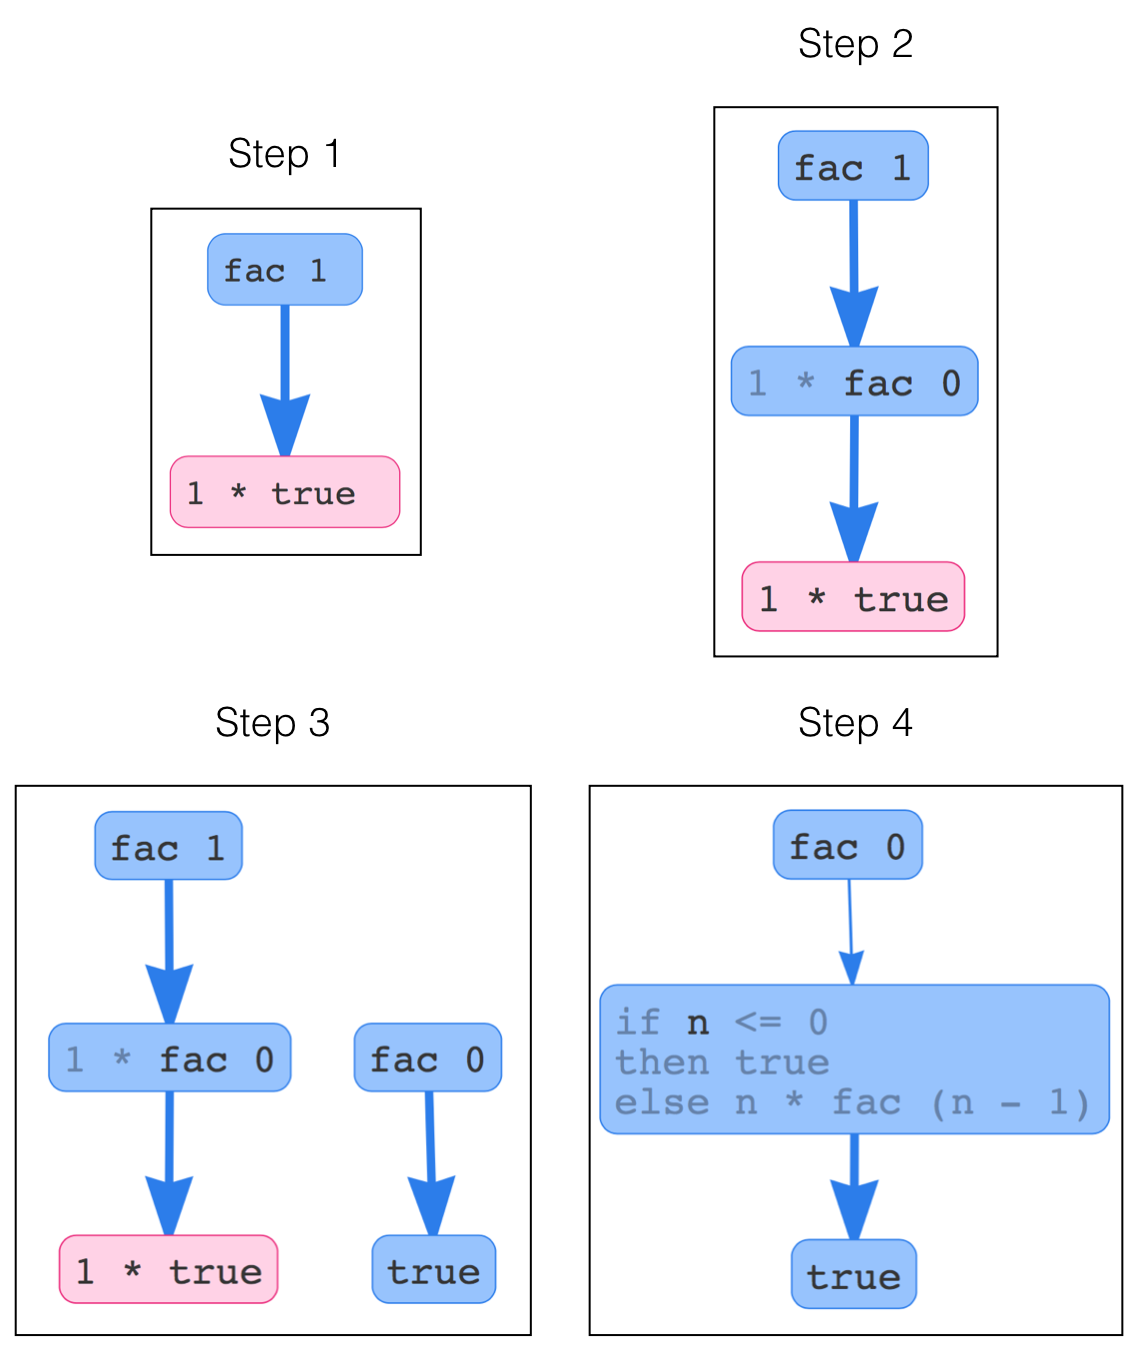
\includegraphics[height=4in]{fac-steps-new.png}
\caption{A sequence of interactions with the trace of
  \texttt{fac 1}. The stuck term is red, in each node the redex is
  highlighted. Thick arrows denote a multi-step transition, thin arrows
  denote a single-step transition. We start in step 1. In step 2 we jump
  forward from the witness to the next function call. In step 3 we step
  into the recursive \texttt{fac 0} call, which spawns a new ``thread''
  of execution. In step 4 we take a single step forward from
  \texttt{fac 0}.}
\label{fig:nanomaly-factorial}
\end{figure}

% \paragraph{Visualization Context}
% %
% The \emph{visualization context} of each expression $e$
% in the visualization state $\vstate$ is the (unique) linear chain
% in which the expression $e$ belongs.
% %
% We write $\vroot{\vstate}{e}$ for the \emph{first} (or root)
% expression appearing in the visualization context of $e$ in
% $\vstate$.

\paragraph{Commands}
Our debugger supports the following \emph{commands}, each of which
is parameterized by a single expression (vertex) selected from the
(current) visualization state:
%
\begin{itemize}
%
\item \stepforwardsym, \stepbackwardsym:
      show the result of a single step forward or backward;
%
\item \jumpforwardsym, \jumpbackwardsym:
      show the result of taking multiple steps (a \emph{``big''} step)
      up to the first function call, or return, forward or backward
      respectively;
%
\item \stepintosym:
      show the result of stepping into a function call in a sub-term,
      isolating it in a new reduction thread; and
%
\item \stepoversym:
      show the result of skipping over a function call in a sub-term.
\end{itemize}

\paragraph{Jump Compression}
%
A \emph{jump compressed} trace is one whose edges are limited to forward
or backward jumps.
% (The sizes of these traces is equal to the jump
% metric below.)
%
In our experience, jump compression abstracts many details of the
computation that are often uninteresting or irrelevant to the
explanation.
%
In particular, jump compressed traces hide low-level operations and
summarize function calls as call-return pairs, see
Figure~\ref{fig:fac-jump} for a variant of @fac@ that implements the
subtraction as a function call instead of a primitive.
%
\begin{figure}[t]
\centering
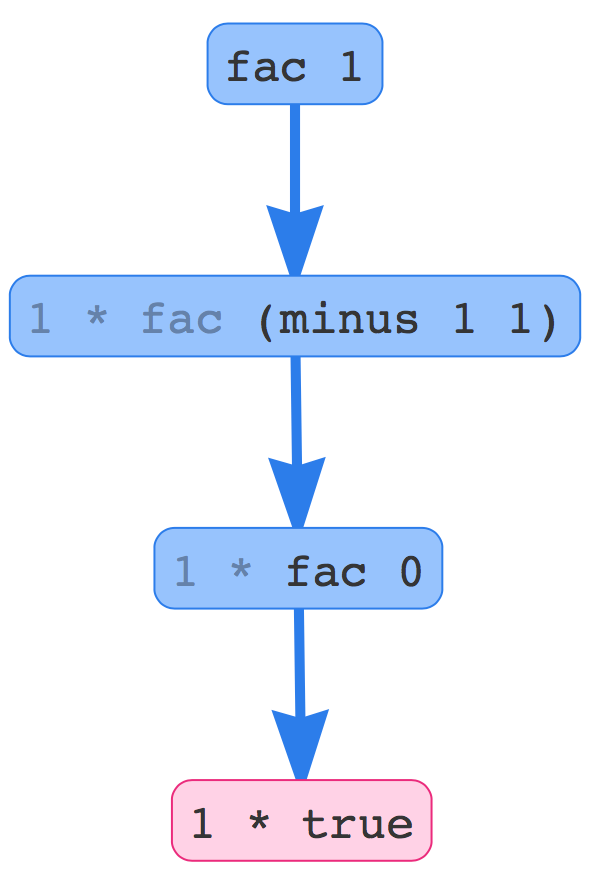
\includegraphics[height=2in]{fac-minus.png}
\caption{Jump-compressed trace of \texttt{fac 1} with subtraction
  implemented as a function call.}
\label{fig:fac-jump}
\end{figure}
%
Once users have identified interesting call-return pairs, they can
step into those calls and proceed with more fine-grained steps.
%
% Expanding the initial visualization to a jump-compressed trace is often
% an ideal first step;
% % expanding a jump-compressed traces ideal for the initial state of the
% they provide a concise overview of the execution and allow the user to
% step directly into an interesting function call, at which point the can
% proceed with more fine-grained steps.
%
Note that jump compressed traces are not quite the same as
stack-traces as they show \emph{all} function calls, including
those that returned successfully.
%
% For example, the display on the bottom-left in Figure~\ref{fig:factorial} shows
% a jump-compressed trace, of size 4. The full trace for
% the same example (on the right of the Figure~\ref{fig:factorial}) has size 19.


% \RJ{add para about jump-compressed traces + example. include full trace and compressed trace.
% could merge with example in overview.}

% \begin{figure*}[t]
\[
\begin{array}{lcl}
\stepforward{\vstate}{e}  & \defeq
  & e' \quad \mbox{where } \singlestep{e}{e'} \in \tr \\ \\

\stepbackward{\vstate}{e} & \defeq
  & e' \quad \mbox{where } \singlestep{e'}{e} \in \tr \mbox{ and } e' \in \vpath{\vstate}{e} \\ \\

\jumpforward{\vstate}{e} & \defeq
  & \begin{cases}
    e'                         & \mbox{if } e' = \eapp{v}{v'} \\
    \jumpforward{\vstate}{e'}  & \text{otherwise}
    \end{cases}
    \mbox{\qquad where } e' = \stepforward{\vstate}{e} \\ \\

\jumpbackward{\vstate}{e} & \defeq
  & \begin{cases}
    e'                         & \mbox{if } e' = \eapp{v}{v'} \\
    \jumpbackward{\vstate}{e'} & \text{otherwise}
    \end{cases}
    \mbox{\qquad where } e' = \stepbackward{\vstate}{e} \\ \\

\stepinto{\vstate}{e} & \defeq
  & e'\sub{x}{v'} \quad \mbox{if } e = C[\eapp{v}{v'}] \mbox{ and } \singlestep{\eapp{v}{v'}}{e'\sub{x}{v'}}  \\ \\

\stepover{\vstate}{e} & \defeq
  & C[v] \quad \mbox{if } e = C[\eapp{v_1}{v_2}] \mbox{ and } \multistep{\eapp{v_1}{v_2}}{v} \in \tr \\[0.25in]

\vpath{\vstate}{e} & \defeq
  & \{e' \spmid \multistep{\vroot{\vstate}{e}}{e'} \in \tr
                \mbox{ and }
                \multistep{e'}{e} \in \tr \} \\[0.15in]
\end{array}
\]
\caption{Rules for computing the \emph{next} term given a
         visualization state $\vstate$, selected term $e$
         and command.}
\label{fig:traversing-graph}
\end{figure*}


% \paragraph{Update}
% %
% Figure~\ref{fig:traversing-graph} shows
% how we compute the \emph{next} expression
% (to be added to the visualization state)
% given the current visualization state
% $\vstate$, command $\cmd$ and selected
% expression $e$.
% %
% It is straightforward to then \emph{update}
% the visualization graph by adding the new
% term before (resp.\ after) the selected
% expression $e$ if the command was a step
% or jump forward (resp.\ backward), or
% to create a new visualization context
% if the command was $\stepintosym$.

%%% and \updState{\vstate}{\cmd}{e} then updates the graph
%%% by inserting the new expression appropriately, using
%%% one of the following graph manipulating functions:
%%% %
%%% \putBefore{\vstate}{e}{e'} (resp. \putAfter{\vstate}{e}{e'})
%%% returns the modified version of \vstate\ where $e'$ is the
%%% immediate predecessor of $e$ (resp.\ the immediate successor of $e$);
%%% %
%%% \putRoot{\vstate}{e}{e'} returns the modified version of \vstate
%%% extended with a new root vertex $e$ with successor $e'$.
%%% %
%%% @getNext vs e@ returns the immediate successor of @e@ in $\tr$.
%%% %
%%% @getPrev vs e@ computes the path @p@ between @e@ and its immediate
%%% predecessor in the current visualization, and then returns @e@'s immediate
%%% predecessor along @p@.
%%% %
%%% @getSubterms vs e@ traverses the sub-term edges to decompose an
%%% expression into a list of sub-expressions paired with their context.
%%% %
%%% @applyCtx vs e ctx@ applies @ctx@ to @e@, traversing the sub-term edges
%%% in reverse to find the super-term of @e@.
%%% %
%%% \hbox{@findApp vs e@} builds on top of @getSubterms@ to find the first
%%% application sub-term (if any), \ie the first sub-term that looks like
%%% $\eapp{v_1}{v_2}$.
%%% %
%%% @findVal vs e@ traverses the single-step edges to find the final value
%%% that @e@ reduces to.

% \section{Evaluation: Recasting Type Errors as Runtime Errors}
\section{Evaluation}
\label{sec:evaluation}

We have implemented a prototype of our search procedure and trace
visualization for a purely functional subset of \ocaml\ --- with
polymorphic types and records, but no modules, objects, or polymorphic
variants --- in a tool called \nanomaly.
%
We treat explicit type signatures, \eg @(x : int)@, as
primitive operations that narrow the type of the wrapped value.
%
In our implementation we instantiated \gensym\ with a simple random
generation of values, which we will show suffices for the majority of
type errors.

\paragraph{Evaluation Goals}
%
There are three questions we seek to answer with our evaluation:
%
\begin{enumerate}
\item \emphbf{Witness Coverage}
      How many ill-typed programs can we find witnesses for?
\item \emphbf{Witness Complexity}
      How \emph{complex} are the traces produced by the witnesses?
\item \emphbf{Witness Utility}
      How \emph{helpful} (qualitatively and quantitatively)
      are the witnesses and traces in debugging type errors?
\end{enumerate}

\paragraph{Benchmarks}
We answer the first two questions on two sets of ill-typed programs,
\ie\ programs that were rejected by the \ocaml\ compiler because of a
type error.
%
The first dataset comes from the Spring 2014 undergraduate Programming
Languages (CSE 130) course at UC San Diego.
%
We recorded each interaction with the \ocaml\ top-level system over the
course of the first three assignments (IRB
% \# hidden for blind review),
\#140608),
from which we extracted \ucsdsize\ distinct, ill-typed \ocaml\ programs.
%
The second dataset --- widely used in the literature --- comes from a
graduate-level course at the University of Washington~\cite{Lerner2006-pj},
from which we extracted 284 ill-typed programs.
%
Both datasets contain relatively small programs, the largest being 348
SLoC; however, they demonstrate a variety of functional programming
idioms including (tail) recursive functions, higher-order functions,
polymorphic data types, and expression evaluators.

We answer the third question in two steps.
%
First, we present a qualitative evaluation of \toolname's traces on a
selection of programs drawn from the UCSD dataset.
%
Second, we present a quantitative user study of students in the
University of Virginia's Spring 2016 undergraduate Programming Languages
(CS 4501) course.
%
As part of an exam, we presented the students with ill-typed \ocaml\
programs and asked them to
%
(1) \emph{explain} the type error, and
%
(2) \emph{fix} the type error (IRB \#2014009900).
%
For each problem the students were given the ill-typed program and
either \ocaml's error message or \toolname's jump-compressed trace.


\subsection{Witness Coverage}
\label{sec:eval:witness-coverage}
%
We ran our search algorithm on each program for 1,000 iterations, with
the entry point set to the function that \ocaml\ had identified as
containing a type error.
%
Due to the possibility of non-termination we set a timeout of one minute
total per program.
%
% Due to the possibility of non-termination we set a limit on the number
% of reductions to perform, increasing in 500-step increments from 500
% steps to 3,000 steps total.
%
We also added a na{\"\i}ve check for infinite recursion; at each recursive
function call we check whether the new arguments are identical to the
current arguments.
%
If so, the function cannot possibly terminate and we report an error.
%
While not a \emph{type error}, infinite recursion is still a clear bug
in the program, and thus valuable feedback for the user.

\begin{figure*}[ht]
\centering
\begin{minipage}{\linewidth}
\centering
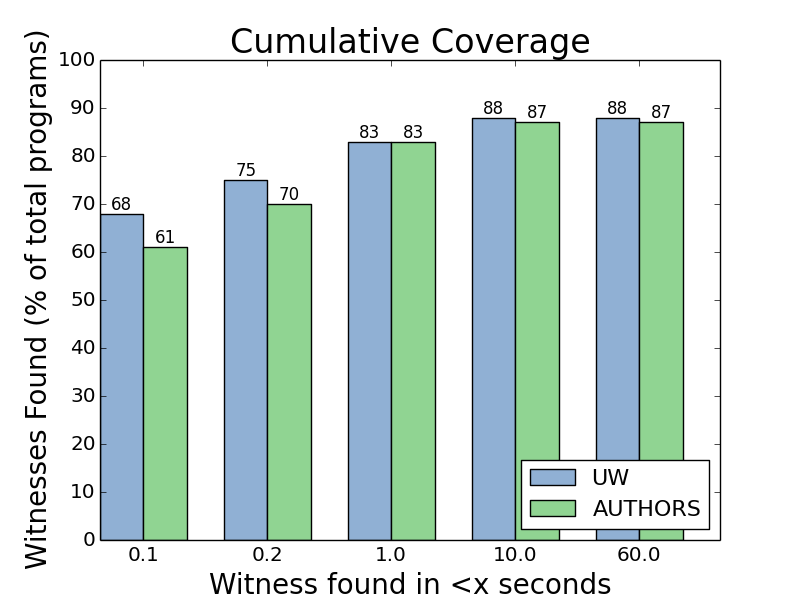
\includegraphics[width=0.49\linewidth]{coverage.png}
% \end{minipage}
% \begin{minipage}{\linewidth}
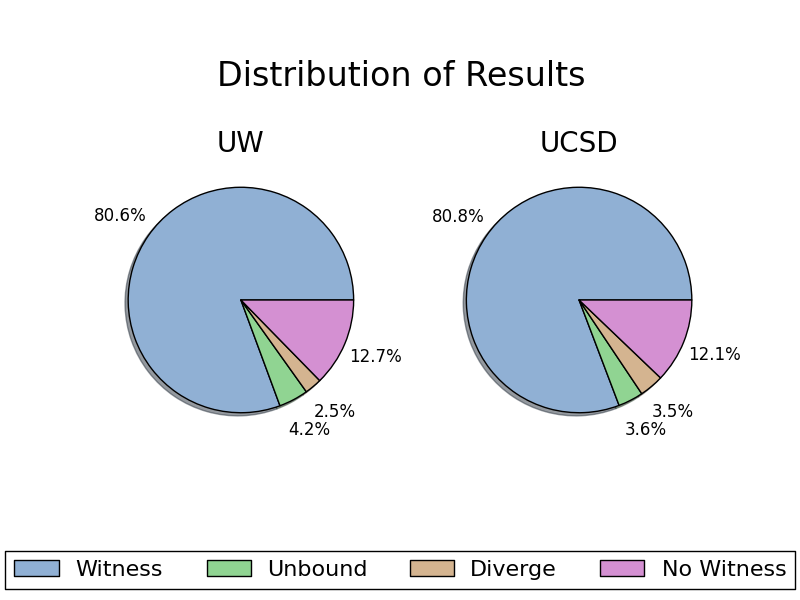
\includegraphics[width=0.49\linewidth]{distrib.png}
\end{minipage}
% \vspace{-8ex}
\caption{Results of our coverage testing and the distribution of test
  outcomes. Our random search successfully finds witnesses for 79--85\% of
  the programs in under one second, improving to 87\% in under
  10 seconds. In both datasets we detect actual type errors about 82\%
  of the time, unbound variables or constructors 3--4\% of the time, and
  diverging loops 2--3\% of the time. For the remaining 11--12\% of the
  programs we are unable to provide any useful feedback.  }
\label{fig:results-witness}
\end{figure*}

\paragraph{Results}
\label{sec:results-witness}
The results of our experiments are summarized in
Figure~\ref{fig:results-witness}.
%
In both datasets our tool was able to find a witness for 83\% of the
programs in under one second, \ie\ fast enough to be integrated as a
compile-time check. If we extend our tolerance to a 10 second timeout,
we hit a maximum of 87\% coverage.
%
Interestingly, while the vast majority of witnesses corresponded to a
type-error, as expected, 3--4\% triggered an unbound variable error (even
though \ocaml\ reported a type error) and 2--3\% triggered an infinite
recursion error.
%
For the remaining 12\% of programs we were unable to provide any useful
feedback as they either completed 1,000 tests successfully, or timed out
after one minute.
%
% XX programs were deemed safe and XX timed out even at 3,000 steps, \ie
% we could not provide any useful feedback for XX\% of the total programs.
%
While a more advanced search procedure, \eg\ dynamic-symbolic execution,
could likely trigger more of the type errors, our experiments suggest that
type errors are coarse enough (or that novice programs are \emph{simple}
enough) that these techniques are not necessary.


\subsection{Witness Complexity}
\label{sec:trace-complexity}

For each of the ill-typed programs for which we could
find a witness, we measure the complexity of the generated
trace according to two metrics.

% \paragraph{Metrics} Thus, our two metrics are:
% size of the full trace,
% \ie the number of small-step reductions, and the size of the jump-compressed
% version of the trace.
%
\begin{enumerate}
\item \emphbf{Single-step Metric} The size of the trace after expanding
  all of the single-step edges from the witness to the stuck term, and
  % This can be thought of as a worst-case
  % complexity, \ie ``How big is the fully-expanded trace?''
\item \emphbf{Jump-compressed Metric} The size of the jump-compressed trace.
\end{enumerate}


% \item \ES{others?}
%
\begin{figure*}[ht]
\centering
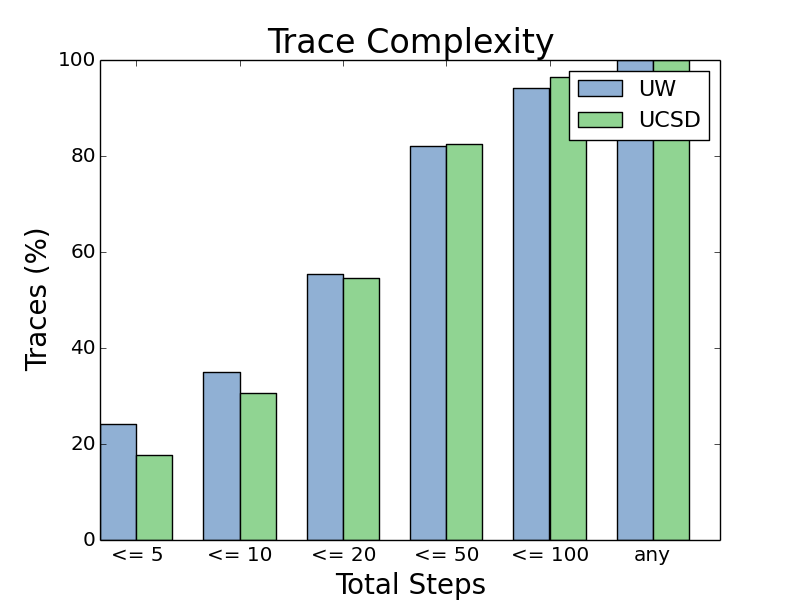
\includegraphics[width=0.49\linewidth]{trace_size_step.png}
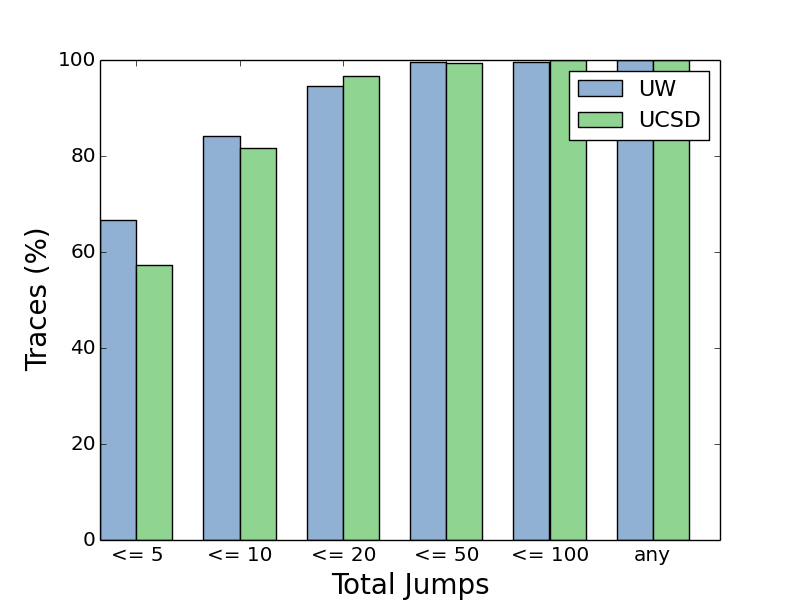
\includegraphics[width=0.49\linewidth]{trace_size_jump.png}
\caption{Complexity of the generated traces. 81\% of the combined traces
  have a jump complexity of at most 10, with an average complexity of 7
  and a median of 5.}
\label{fig:results-complexity}
\end{figure*}
%

\paragraph{Results}
\label{sec:results-complexity}
The results of the experiment are summarized in
Figure~\ref{fig:results-complexity}.
%
The average number of single-step reductions per trace is 31 for the
\ucsdbench\ dataset (35 for the \uwbench\ dataset) with a maximum of
2,745 (986 for \uwbench) and a median of 17 (also 17 for \uwbench).
%
The average number of jumps per trace is 7 (also 7 for \uwbench) with a
maximium of 353 (185 for \uwbench) and a median of 4 (also 4 for
\uwbench).
%
In both datasets 80\% or more traces have at most 10 jumps.
%


\subsection{Witness Utility}
\section{The Advantage Of Traces}\label{sec:advantage-traces}

Next, we present a \emph{qualitative} evaluation that compares
the explanations provided by \toolname's dynamic witnesses with
the static reports produced by the \ocaml\ compiler and \sherrloc,
a state-of-the-art fault localization approach~\cite{zhang_toward_2014}.
%
In particular, we illustrate, using a series of examples drawn
from student programs in the \ucsdbench\ dataset how \toolname's
jump-compressed traces can get to the heart of the error by
%
highlighting the conflicting values that cause the program to get
stuck, rather that blaming a single one,
%
showing the steps necessary to reach the stuck state, and
%
not assuming that a function is correct just because it type-checks.
%
For each example we will present
(1)~the code,
(2)~the error message returned \ocaml,
(3)~the error locations returned by \ocaml\ (underlined) and \sherrloc\ (in bold),
\footnote{When the locations from \ocaml\ and \sherrloc\ overlap,
we just underline the relevant code.}
(4)~the jump-compressed trace produced by \toolname.

% \begin{figure*}[ht]
% \centering
% \begin{minipage}{0.49\linewidth}
% \centering


\paragraph{Example: Recursion with Bad Operator}
The recursive function @sqsum@ should square each
element of the input list and then compute the sum
of the result.
%
\begin{ecode}
  let rec sqsum xs = match xs with
    | [] -> 0
    | h::t -> __(sqsum t)__ @ (h * h)
\end{ecode}
%
Unfortunately the student has used the list-append
operator |@| instead of \texttt{+} to compute the sum.
%
Both \ocaml\ and \sherrloc\ blame the \emph{wrong location},
namely the recursive call @sqsum t@ with the message
%
\begin{verbatim}
  This expression has type
    int
  but an expression was expected of type
    'a list
\end{verbatim}
%
\toolname\ produces the following trace showing how the evaluation of
@sqsum [1]@ gets stuck:
%
\begin{center}
  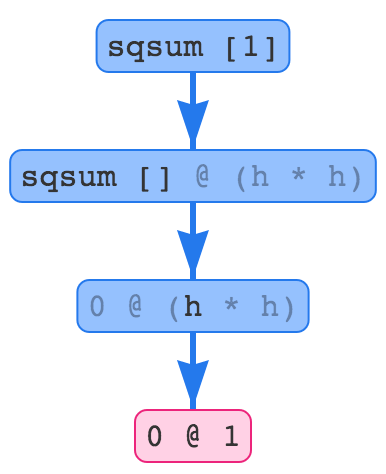
\includegraphics[height=125px]{sqsum.png}
\end{center}
%
The figure highlights the entire stuck term
(not just the recursive call), emphasizing
the \emph{conflict} between @int@ and @list@
rather than assuming one or the other is correct.

\paragraph{Example: Recursion with Bad Base Case}
%
The function @sumList@ should add up
the elements of its input list.
%
\begin{ecode}
  let rec sumList xs = match xs with
    | []    -> ==[]==
    | y::ys -> y + __sumList ys__
\end{ecode}
%
Unfortunately, in the base case, it returns @[]@
instead of @0@.
%
\sherrloc\ blames the base case, and \ocaml\
assumes the base case is correct and blames
the \emph{recursive call} on line 3:
%
\begin{verbatim}
  This expression has type
    'a list
  but an expression was expected of type
    int
\end{verbatim}
%
Both of the above are parts of the full story, which
is succinctly summarized by \toolname's trace showing
how @sumList [1; 2]@ gets stuck at @2 + []@.
%
\begin{center}
  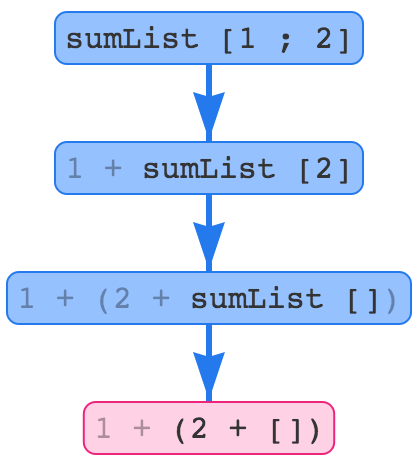
\includegraphics[height=125px]{sumlist.png}
\end{center}
%
The trace clarifies immediately (via the third step)
that the @[]@ is the result of the recursive call
@sumList []@, and shows how it is incompatible with
the subsequent \texttt{+} operation.

%% ES: append is actually a bit problematic as we don't find the nice
%% append [1] [2] witness. instead we could find something like
%% append [_] [], but it's not as clear IMO
% Our next example is the @append@ function, which should concatenate the
% two input lists.
% %
% \begin{ecode}
% let append xs ys = match xs with
%   | []   -> ys
%   | h::t -> h :: __t__ :: ys
% \end{ecode}
% %
% The student has forgotten to make a recursive call to @append@, and
% instead tries to cons the tail @t@ directly onto the second list @ys@.
% Consing @h@ back onto the result causes \ocaml to attempt to construct
% the infinite type @'a = 'a list@, triggering an \emph{occurs-check}
% error.
% %
% \begin{verbatim}
% Error: This expression has type
%          'a list
%        but an expression was expected of type
%          'a
%        The type variable 'a occurs inside 'a list
% \end{verbatim}
% %
% %
% \begin{center}
%   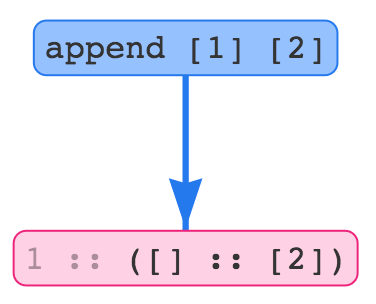
\includegraphics[height=75px]{append.png}
% \end{center}

\paragraph{Example: Bad Helper Function that Type-Checks}
%
The function @digitsOfInt@ is supposed to return a list of
the digits of the input integer.
%
\begin{ecode}
  let append x xs =
    match xs with
    | [] -> [x]
    | _  -> x :: xs

  let rec digitsOfInt n =
    if n <= 0 then
      []
    else
      append (==digitsOfInt (n / 10)==)
             [__n mod 10__]
\end{ecode}
%
Unfortunately, the student's @append@ function \emph{conses} an element
onto a list instead of appending two lists.
%
Though incorrect, @append@ still type-checks and thus \ocaml and
\sherrloc blame the \emph{use-site} on line 10.
%
\begin{verbatim}
  This expression has type
    int
  but an expression was expected of type
    'a list
\end{verbatim}
%
\toolname, in contrast, makes no asummptions about @append@ and produces
a trace that illustrates the true error on line 4, by
highlighting the conflict in consing a list onto a list of integers.
%
\begin{center}
  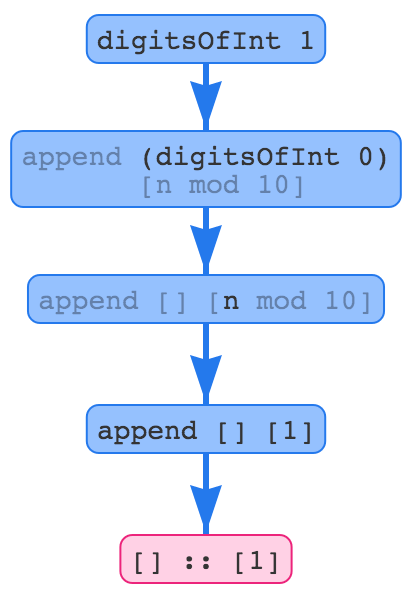
\includegraphics[height=175px]{digitsOfInt.png}
\end{center}
%

\paragraph{Example: Higher-Order Functions}
%
The higher-order function @wwhile@ is supposed
to emulate a traditional while-loop. It takes
a function @f@ and repeatedly calls @f@ on the
first element of its output pair, starting with
the initial value @b@, until the second element
is @false@.
%
\begin{ecode}
  let rec wwhile (f,b) =
    match f with
    | (z, false) -> z
    | (z, true)  -> wwhile (f, z)

  let f x =
    let xx = x * x in
    (xx, (xx < 100))

  let _ = wwhile (__f__, 2)
\end{ecode}
%
Unfortunately, the student has forgotten to \emph{apply}
@f@ at all on line 2, and just matches it directly against
a pair.
This faulty definition of @wwhile@ still typechecks however,
and hence, are ``assumed'' to be correct by and both \ocaml\
and \sherrloc\ which blame the \emph{use-site} on line 10.
%
\begin{verbatim}
  This expression has type
    int -> int * bool
  but an expression was expected of type
    'a * bool
\end{verbatim}
%
\toolname\ synthesizes a trace that draws the eye to the
true error: the @match@ expression on line 2, and highlights
the conflict in matching a function against a pair pattern.
%
\begin{center}
  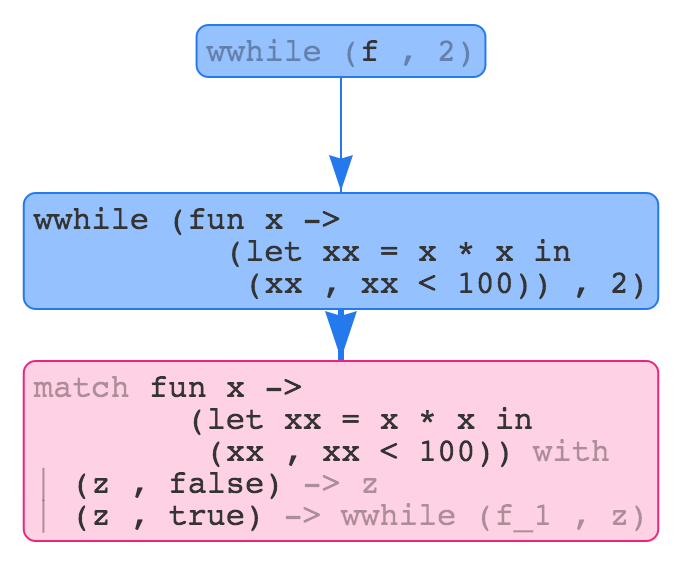
\includegraphics[height=150px]{wwhile.png}
\end{center}
%
By highlighting conflicting values (\ie\ the source and sink
of the problem) and not making any assumptions, \toolname\
focusses the user's attention on the piece of code that is
actually relevant to the error.


%%% Local Variables:
%%% mode: latex
%%% TeX-master: "main"
%%% End:


\subsubsection{Quantitative}
\label{sec:user-study}
% Finally, to test the explanatory power of our jump-compressed traces, we
% ran a user study (IRB \#2014009900) at the University of Virginia (UVA).
% %
% We included four problems in an exam in the Spring session of UVA's
% undergraduate Programming Languages course (CS 4501).
% %
% We presented the 60 students in the course with ill-typed \ocaml\
% programs and asked them to
% %
% (1) \emph{explain} the type error, and
% %
% (2) \emph{fix} the type error.
% %
% For each problem the student was given the ill-typed program and
% either \ocaml's error message or \toolname's jump-compressed trace.
%
We assigned four problems to the ($n=60$) students in the course: the
@sumList@, @digitsOfInt@, and @wwhile@ programs from
\S~\ref{sec:advantage-traces}, as well as the following @append@ program
%
\begin{ecode}
  let append x l =
    match x with
    | []   -> l
    | h::t -> h :: t :: l
\end{ecode}
%
which triggers an occurs-check error on line 4.
%
For each problem the students were given the ill-typed program and
either \ocaml's error message or \toolname's jump-compressed trace.
%
Due to the nature of an in-class exam, not every student answered every
question; we received between 13 and 28 (out of a possible 30) responses
for each problem-tool pair.

We then instructed four annotators (one of whom is an author, the other
three are teaching assistants at UCSD) to classify the answers as
correct or incorrect.
%
We performed an inter-rater reliability (IRR) analysis to determine the
degree to which the annotators consistently graded the exams.
%
As we had more than two annotators assigning nominal (``correct'' or
``incorrect'') ratings we used Fleiss' kappa~\cite{Fleiss1971-du} to
measure IRR.\@
%
Fleiss' kappa is measured on a scale from $1$, indicating total
agreement, to $-1$, indicating total disagreement, with $0$ indicating
random agreement.

\paragraph{Threats to Validity}
\subparagraph{Construct}
%
Measuring understanding is a difficult task; we used the correctness of
the student's explanation of, and fix for, the type error as a proxy for
her understanding, but it is possible that other metrics would produce
different results.

\subparagraph{Internal}
%
We assigned students randomly to two groups. The first group was given
\ocaml's errors for @append@ and \hbox{@digitsOfInt@,} and \toolname's trace
for @sumList@ and @wwhile@. The second group was given the opposite
assignment of errors and traces. This assignment ensured that (1) each
student was given \ocaml and \toolname problems, and (2) each student
was given an ``easy'' and ``hard'' problem for both \ocaml and
\toolname. Students without sufficient knowledge of \ocaml could affect
the results, as could the time-constrained nature of an exam. For these
reasons we excluded any answers left blank from our analysis.

\subparagraph{External}
%
Our experiment is based on students in the process of learning \ocaml,
and thus may not generalize to all developers. The four
programs we used were chosen manually, via a random selection and
filtering of the programs in the \ucsdbench dataset. In some cases we made
minor simplifying edits (\eg alpha-renaming, dead-code removal) to the
programs to make them more understandable in the short timeframe of an
exam; however, we never altered the resulting type-error. A different
selection of programs may lead to different results.

\subparagraph{Conclusion}
%
We collected exams from 60 students, though due to the nature of the
study not every student completed every problem.
%
The number of complete submissions ranges from 13 (for the \toolname
version of @wwhile@) to 28 (for the \ocaml version of @sumList@), out of
a maximum of 30 per program-tool pair.
%
Collecting more responses per test pair was not possible, as it
would require having students answer the same problem twice (once with
\ocaml and once with \toolname).


\paragraph{Results}
%
Figure~\ref{fig:results-user-study} summarizes a single annotator's
results, which show that students given \toolname's jump-compressed
trace were consistently more likely to correctly explain
and fix the type error than those given \ocaml's error message.
%
Across each problem the \toolname responses were marked correct
$10-30\%$ more often than the \ocaml responses, which suggests that
the students who had access to \toolname's traces had a better
understanding of the type errors.
%
The measured kappa values were $\kappa = 0.72$ for the explanations and
$\kappa = 0.83$ for the fixes; while there is no formal notion for what
consititutes strong agreement~\cite{Krippendorff2012-wd}, kappa values
above $0.60$ are often called ``substantial''
agreement~\cite{Landis1977-ey}.
%
\begin{figure*}[ht]
\centering
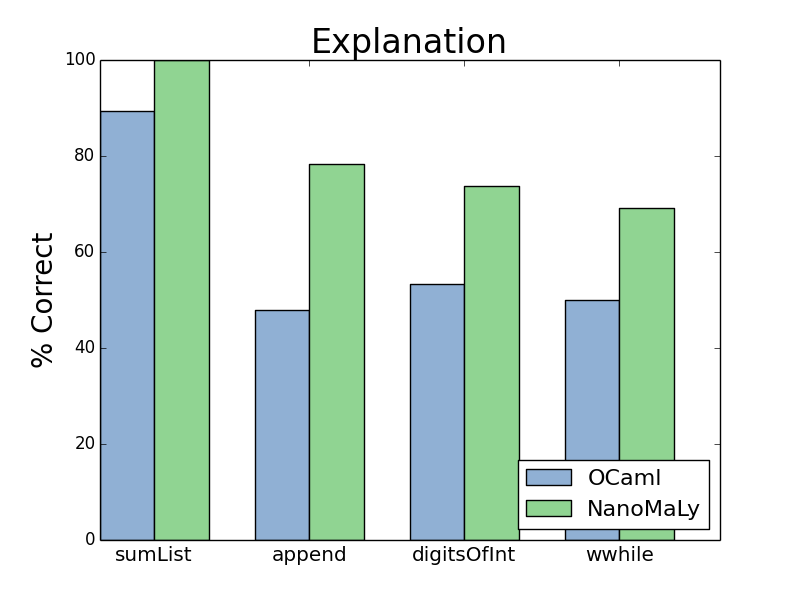
\includegraphics[width=0.49\linewidth]{user-study-reason.png}
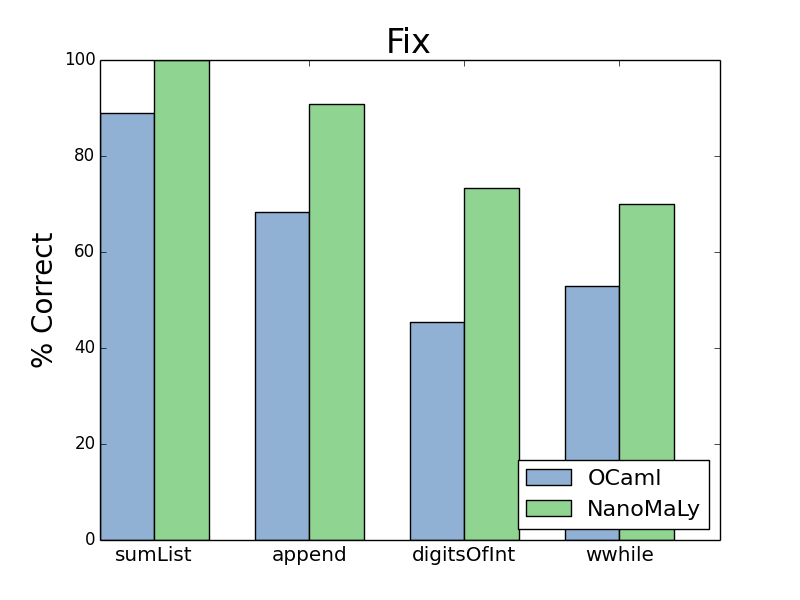
\includegraphics[width=0.49\linewidth]{user-study-fix.png}
\caption{A classification of students' explanations and fixes for type
  errors, given either \ocaml's error % message
  or \toolname's
  jump-compressed trace. The students given \toolname's jump-compressed
  trace consistently scored better ($\ge 10\%$) than those given \ocaml's type
  error.}
\label{fig:results-user-study}
\end{figure*}
%

\subsection{Discussion}
\label{sec:discussion}

To summarize, our experiments demonstrate that \nanomaly finds witnesses
to type errors: (1) with high coverage in a timespan amenable to
compile-time analysis, (2) with traces that have a low average
complexity of 7 jumps, and (3) that are more helpful to novice
programmers than traditional type error messages.

There are, of course, drawbacks to our approach. Four that stand out
are: (1) coverage limits due to random generation, (2) the inability to
handle certain instances of infinite types, (3) dealing with an
explosion in the size of generated traces, and (4) handling ad-hoc
polymorphism.

\paragraph{Random Generation}
Random test generation has difficulty generating highly constrained
values, \eg\ red-black trees or a pair of equal integers. If the type
error is hidden behind a complex branch condition \nanomaly\ may not be
able to trigger it. Exhaustive testing and dynamic-symbolic execution
can address this short-coming by performing an exhaustive search for
inputs (\emph{resp}.\ paths through the program). As our experiments
show, however, novice programs do not appear to require more advanced
search techniques, likely because the novice programs tend to be simple.

\paragraph{Infinite Types}
Our implementation does check for infinite types inside \forcesym, but
there are some degenerate cases where it is unable to detect
them. Consider, the following buggy @replicate@
%
\begin{code}
  let rec replicate n x =
    if n <= 0 then
      []
    else
      replicate (n-1) [x]
\end{code}
%
This code produces a nested list (with @n@ levels of nesting) containing
a single copy of @x@, instead of a list with @n@ copies of @x@. \ocaml\
detects a cyclic \hbox{@'a = 'a list@} constraint in the recursive call
and throws a type error, whereas \nanomaly\ happily % recurses @n@ times to
produces the nested list.  Strictly speaking, this function itself cannot
``go wrong'', the program would not get stuck until a \emph{client}
attempted to use the result expecting a flat list. But this is not very
satisfying as @replicate@ is clearly to blame. Furthermore, in our
experience, infinite-type errors are often difficult to %some of the more difficult ones to
debug (and to explain to novices), so better support for this scenario
would be useful.

\paragraph{Trace Explosion}
Though the average complexity of our generated traces is low in terms of
jumps, there are some extreme outliers.
%
We cannot reasonably expect a novice user to explore a trace containing
50+ terms and draw a conclusion about which pieces contributed to the
bug in their program.
%
Enhancing our visualization to slice out program paths relevant to
specific values~\cite{Perera2012-dy}, would likely help alleviate this
issue, allowing users to highlight a confusing value and ask: ``Where
did this come from?''

\paragraph{Ad-hoc Polymorphism}
Our approach can only support ad-hoc polymorphism (\eg\ type-classes in
\haskell\ or polymorphic comparison functions in \ocaml) in limited cases
where we have enough typing information at the call-site to resolve the
overloading. For example, consider the @n <= 0@ test in our @fac@ example.
@<=@ is polymorphic in \ocaml, but in this case we can make progress because
the literal @0@ is not. If we parameterized @fac@ by a lower bound, \eg
%
\begin{code}
  let rec fac n m =
    if n <= m then
      1
    else
      n * fac (n - 1) m
\end{code}
%
and called @fac@ with two holes, we would get stuck at the @n <= m@
test; not because of a type error, but because all we know about
@n@ and @m@ at that point is that they must have the same (unknown)
type.

This issue is uncommon in \ocaml\ (we did not detect a single instance
of it across all of our benchmarks), but it would surely be exacerbated
by a language like \haskell, which makes heavy use of overloading. We
suspect that dynamic-symbolic execution would allow us to handle ad-hoc
polymorphism, but defer a proper treatment to future work.

% \begin{itemize}
% \item benchmarks: our data + seminal data
% \item both cases: \textbf{random} search sufficient to trigger runtime crash in 80\% of programs
% \item how many of the ``safe'' programs are actually safe??
% \end{itemize}

%%% Local Variables:
%%% mode: latex
%%% TeX-master: "main"
%%% End:
%!TEX root = main.tex

% \section{The Advantage Of Traces}
\label{sec:advantage-traces}
Finally, having shown that \toolname produces small traces in an
efficient manner, let us discuss the explanatory power of traces
compared with typical type error messages. In this section we will
present a qualitative evaluation of \toolname's jump-compressed traces
on a series of examples drawn from real student programs in the
\ucsdbench dataset. For each example we will present the code, a
jump-compressed trace produced by \toolname, and the type error produced
by the \ocaml compiler.

\begin{figure*}[ht]
\centering
\begin{minipage}{0.49\linewidth}
\centering
\begin{ecode}
let rec sqsum xs = match xs with
  | [] -> 0
  | h::t -> __(sqsum t)__ @ (h * h)
\end{ecode}
% File "sqsum.ml", line 3, characters 12-21:
\begin{verbatim}
Error: This expression has type
         int
       but an expression was expected of type
         'a list
\end{verbatim}
\end{minipage}
\begin{minipage}{0.49\linewidth}
\centering
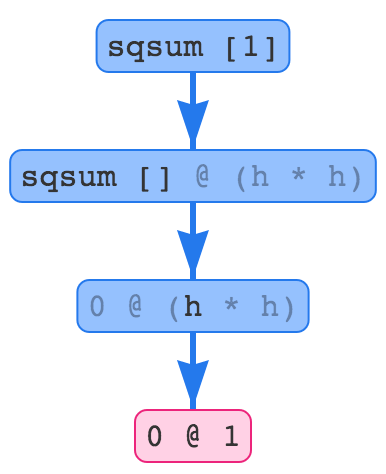
\includegraphics[height=125px]{sqsum.png}
\end{minipage}
\caption{\texttt{sqsum xs} should square each element of \texttt{xs} and
  then compute the sum of the result, but the student has used the
  list-append operator |@| instead of \texttt{+} to compute the
  sum. \ocaml blames the recursive call \texttt{sqsum t} (underlined
  above) for being an \texttt{int} instead of a \texttt{list}.
  \toolname's jump-compressed trace draws the eye to the
  entire term \texttt{0 }|@|\texttt{ 1}.}
\label{fig:traces}
\end{figure*}

\begin{figure*}[ht]
\centering
\begin{minipage}{0.49\linewidth}
\centering
\begin{ecode}
let rec sumList xs = match xs with
  | []    -> []
  | y::ys -> y + __sumList ys__
\end{ecode}
% File "sumList.ml", line 3, characters 17-27:
\begin{verbatim}
Error: This expression has type
         'a list
       but an expression was expected of type
         int
\end{verbatim}
\end{minipage}
\begin{minipage}{0.49\linewidth}
\centering
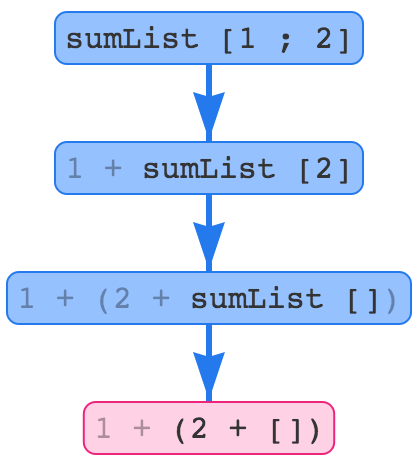
\includegraphics[height=125px]{sumlist.png}
\end{minipage}
\caption{\texttt{sumList xs} should sum the elements of \texttt{xs}, but
  the student has returned \texttt{[]} in the base case instead of
  \texttt{0}. \ocaml deduces from the base case that \texttt{sumList}
  must return a \texttt{list} and thus blames the recursive call on line
  3 for producing a \texttt{list} instead of an  \texttt{int}.
  \toolname's jump-compressed trace highlights the clash
  between the \texttt{[]} and the \texttt{+}, but also demonstrates in
  the third step that \texttt{sumList []} reduces to \texttt{[]}, which
  clarifies that the conflict is between the base case and recursive
  case.}
\label{fig:traces}
\end{figure*}

\begin{figure*}[ht]
\centering
\begin{minipage}{0.49\linewidth}
\centering
\begin{ecode}
let append xs ys = match xs with
  | []   -> ys
  | h::t -> h :: __t__ :: ys
\end{ecode}
% File "append.ml", line 3, characters 17-18:
\begin{verbatim}
Error: This expression has type
         'a list
       but an expression was expected of type
         'a
       The type variable 'a occurs inside 'a list
\end{verbatim}
\end{minipage}
\begin{minipage}{0.49\linewidth}
\centering
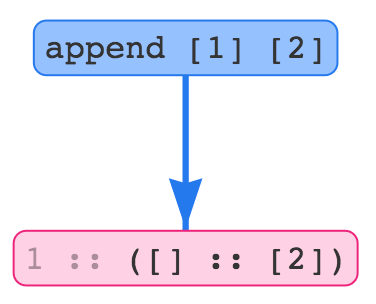
\includegraphics[height=75px]{append.png}
\end{minipage}
\caption{\texttt{append xs ys} should concatenate the two input lists,
  but the student has tried to cons the tail of \texttt{xs} onto
  \texttt{ys} instead of making a recursive call to \texttt{append}.
  \ocaml blames \texttt{t} on line 3 for being a \texttt{'a list}
  instead of a \texttt{'a}, prompting an \emph{occurs-check}
  error. \toolname shows, more concretely, that \texttt{[] :: [2]} gets
  stuck because lists are homogeneous and \texttt{[]} is not an
  \texttt{int}.}
\label{fig:traces}
\end{figure*}

\begin{figure*}[ht]
\centering
\begin{minipage}{0.49\linewidth}
\centering
\begin{ecode}
let rec wwhile (f,b) =
  match f with
  | (z, false) -> z
  | (z, true)  -> wwhile (f, z)

let f x =
  let xx = x * x in
  (xx, (xx < 100))

let _ = wwhile (__f__, 2)
\end{ecode}
% File "wwhile.ml", line 10, characters 16-17:
\begin{verbatim}
Error: This expression has type
         int -> int * bool
       but an expression was expected of type
         'a * bool
\end{verbatim}
\end{minipage}
\begin{minipage}{0.49\linewidth}
\centering
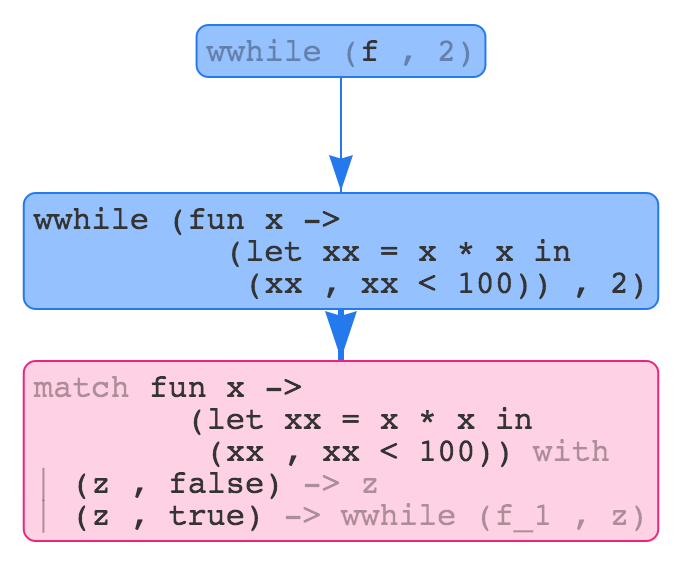
\includegraphics[height=150px]{wwhile.png}
\end{minipage}
\caption{\texttt{wwhile (f, b)} should repeatedly apply the function
  \texttt{f} to the first element of its result pair, starting with the
  initial input \texttt{b}, until the second element is \texttt{false}.
  Unfortunately, the student has forgotten to apply \texttt{f} at all on
  line 2, and just matches it directly against a pair. This faulty
  definition of \texttt{wwhile} still typechecks however, and \ocaml
  thus blames the \emph{call-site} on line 10. \toolname makes no
  assumptions about the input code and quickly draws the eye to the true
  error, the \texttt{match} expression, and highlights the conflict in
  matching a function against a pair pattern.}
\label{fig:traces}
\end{figure*}














%%% Local Variables:
%%% mode: latex
%%% TeX-master: "main"
%%% End:

% \section{The Advantage Of Traces}\label{sec:advantage-traces}

Next, we present a \emph{qualitative} evaluation that compares
the explanations provided by \toolname's dynamic witnesses with
the static reports produced by the \ocaml\ compiler and \sherrloc,
a state-of-the-art fault localization approach~\cite{zhang_toward_2014}.
%
In particular, we illustrate, using a series of examples drawn
from student programs in the \ucsdbench\ dataset how \toolname's
jump-compressed traces can get to the heart of the error by
%
highlighting the conflicting values that cause the program to get
stuck, rather that blaming a single one,
%
showing the steps necessary to reach the stuck state, and
%
not assuming that a function is correct just because it type-checks.
%
For each example we will present
(1)~the code,
(2)~the error message returned \ocaml,
(3)~the error locations returned by \ocaml\ (underlined) and \sherrloc\ (in bold),
\footnote{When the locations from \ocaml\ and \sherrloc\ overlap,
we just underline the relevant code.}
(4)~the jump-compressed trace produced by \toolname.

% \begin{figure*}[ht]
% \centering
% \begin{minipage}{0.49\linewidth}
% \centering


\paragraph{Example: Recursion with Bad Operator}
The recursive function @sqsum@ should square each
element of the input list and then compute the sum
of the result.
%
\begin{ecode}
  let rec sqsum xs = match xs with
    | [] -> 0
    | h::t -> __(sqsum t)__ @ (h * h)
\end{ecode}
%
Unfortunately the student has used the list-append
operator |@| instead of \texttt{+} to compute the sum.
%
Both \ocaml\ and \sherrloc\ blame the \emph{wrong location},
namely the recursive call @sqsum t@ with the message
%
\begin{verbatim}
  This expression has type
    int
  but an expression was expected of type
    'a list
\end{verbatim}
%
\toolname\ produces the following trace showing how the evaluation of
@sqsum [1]@ gets stuck:
%
\begin{center}
  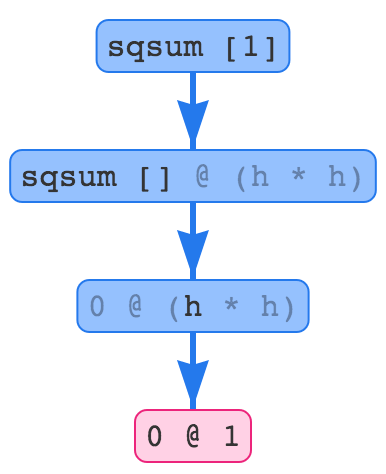
\includegraphics[height=125px]{sqsum.png}
\end{center}
%
The figure highlights the entire stuck term
(not just the recursive call), emphasizing
the \emph{conflict} between @int@ and @list@
rather than assuming one or the other is correct.

\paragraph{Example: Recursion with Bad Base Case}
%
The function @sumList@ should add up
the elements of its input list.
%
\begin{ecode}
  let rec sumList xs = match xs with
    | []    -> ==[]==
    | y::ys -> y + __sumList ys__
\end{ecode}
%
Unfortunately, in the base case, it returns @[]@
instead of @0@.
%
\sherrloc\ blames the base case, and \ocaml\
assumes the base case is correct and blames
the \emph{recursive call} on line 3:
%
\begin{verbatim}
  This expression has type
    'a list
  but an expression was expected of type
    int
\end{verbatim}
%
Both of the above are parts of the full story, which
is succinctly summarized by \toolname's trace showing
how @sumList [1; 2]@ gets stuck at @2 + []@.
%
\begin{center}
  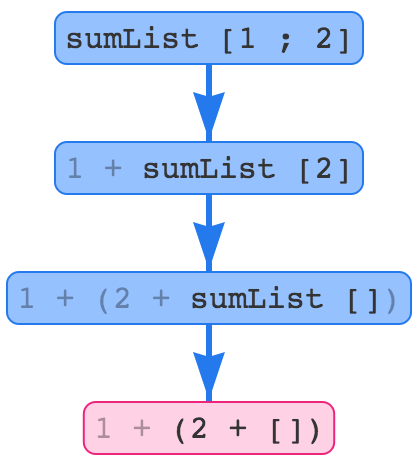
\includegraphics[height=125px]{sumlist.png}
\end{center}
%
The trace clarifies immediately (via the third step)
that the @[]@ is the result of the recursive call
@sumList []@, and shows how it is incompatible with
the subsequent \texttt{+} operation.

%% ES: append is actually a bit problematic as we don't find the nice
%% append [1] [2] witness. instead we could find something like
%% append [_] [], but it's not as clear IMO
% Our next example is the @append@ function, which should concatenate the
% two input lists.
% %
% \begin{ecode}
% let append xs ys = match xs with
%   | []   -> ys
%   | h::t -> h :: __t__ :: ys
% \end{ecode}
% %
% The student has forgotten to make a recursive call to @append@, and
% instead tries to cons the tail @t@ directly onto the second list @ys@.
% Consing @h@ back onto the result causes \ocaml to attempt to construct
% the infinite type @'a = 'a list@, triggering an \emph{occurs-check}
% error.
% %
% \begin{verbatim}
% Error: This expression has type
%          'a list
%        but an expression was expected of type
%          'a
%        The type variable 'a occurs inside 'a list
% \end{verbatim}
% %
% %
% \begin{center}
%   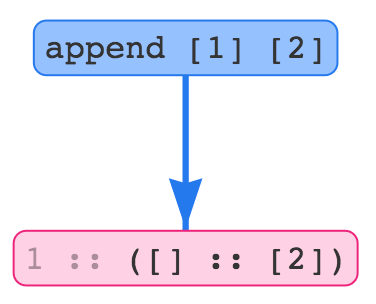
\includegraphics[height=75px]{append.png}
% \end{center}

\paragraph{Example: Bad Helper Function that Type-Checks}
%
The function @digitsOfInt@ is supposed to return a list of
the digits of the input integer.
%
\begin{ecode}
  let append x xs =
    match xs with
    | [] -> [x]
    | _  -> x :: xs

  let rec digitsOfInt n =
    if n <= 0 then
      []
    else
      append (==digitsOfInt (n / 10)==)
             [__n mod 10__]
\end{ecode}
%
Unfortunately, the student's @append@ function \emph{conses} an element
onto a list instead of appending two lists.
%
Though incorrect, @append@ still type-checks and thus \ocaml and
\sherrloc blame the \emph{use-site} on line 10.
%
\begin{verbatim}
  This expression has type
    int
  but an expression was expected of type
    'a list
\end{verbatim}
%
\toolname, in contrast, makes no asummptions about @append@ and produces
a trace that illustrates the true error on line 4, by
highlighting the conflict in consing a list onto a list of integers.
%
\begin{center}
  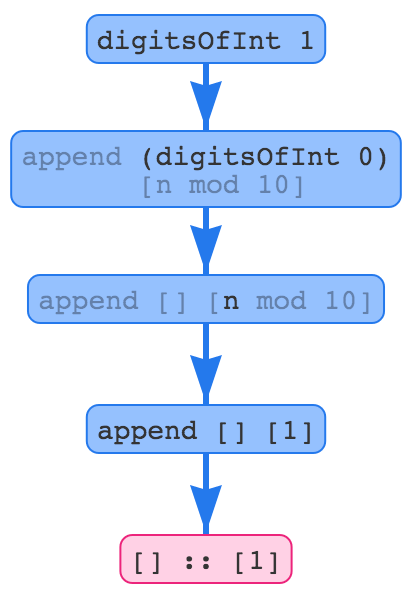
\includegraphics[height=175px]{digitsOfInt.png}
\end{center}
%

\paragraph{Example: Higher-Order Functions}
%
The higher-order function @wwhile@ is supposed
to emulate a traditional while-loop. It takes
a function @f@ and repeatedly calls @f@ on the
first element of its output pair, starting with
the initial value @b@, until the second element
is @false@.
%
\begin{ecode}
  let rec wwhile (f,b) =
    match f with
    | (z, false) -> z
    | (z, true)  -> wwhile (f, z)

  let f x =
    let xx = x * x in
    (xx, (xx < 100))

  let _ = wwhile (__f__, 2)
\end{ecode}
%
Unfortunately, the student has forgotten to \emph{apply}
@f@ at all on line 2, and just matches it directly against
a pair.
This faulty definition of @wwhile@ still typechecks however,
and hence, are ``assumed'' to be correct by and both \ocaml\
and \sherrloc\ which blame the \emph{use-site} on line 10.
%
\begin{verbatim}
  This expression has type
    int -> int * bool
  but an expression was expected of type
    'a * bool
\end{verbatim}
%
\toolname\ synthesizes a trace that draws the eye to the
true error: the @match@ expression on line 2, and highlights
the conflict in matching a function against a pair pattern.
%
\begin{center}
  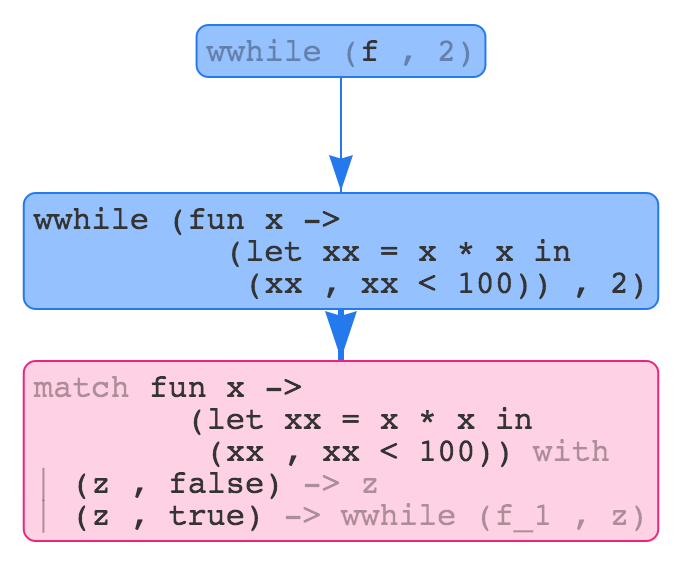
\includegraphics[height=150px]{wwhile.png}
\end{center}
%
By highlighting conflicting values (\ie\ the source and sink
of the problem) and not making any assumptions, \toolname\
focusses the user's attention on the piece of code that is
actually relevant to the error.


%%% Local Variables:
%%% mode: latex
%%% TeX-master: "main"
%%% End:

\section{Related Work}
\label{sec:related-work}
% In this section we connect our work to related efforts on type errors,
% testing, and program exploration.

% \paragraph{Type Errors}
% \label{sec:type-error}

\paragraph{Localizing and Repairing Type Errors}
\label{sec:diagnosis-repair}
% It is well known that
% unification-based type inference procedures can
% produce poor error messages, and in particular, can misidentify the
% \emph{source} of the type error.
%
Many groups have explored techniques to pinpoint the true source
of errors reported by static type checkers.
% unification-based type inference procedures.
%
% \subparagraph{Localization}
The traditional Damas-Milner type inference algorithm~\cite{Damas1982-uw}
reports the first program location where a type mismatch is discovered
(subject to the traversal strategy~\cite{Lee1998-ys}).
%
As a result the error can be reported far away from its
source~\cite{McAdam1998-ub} without enough information to guide the
user.
%
Type-error slicing~\cite{Haack2003-vc,Schilling2011-yf,Rahli2015-tt,Sagonas2013-bf,Gast2004-zd,Neubauer2003-xv}
%treats type inference as a constraint-satisfaction problem and
recognizes this flaw and instead produces a slice of the program
containing \emph{all} program locations that are connected to the type
error.
%
%% \cite{Neubauer2003-xv} present a decidable type system based on
%% discriminative sum types, in which all terms are typeable and type
%% derivations contain all type errors in a program. They then use the
%% typing derivation to slice out the parts of the expression related to
%% each error.
%
Though the program slice must contain the source of the error, it can
suffer from the opposite problem of providing \emph{too much}
information, motivating recent work in ranking the candidate locations.
%
Zhang~\etal~\shortcite{Zhang2014-lv,Zhang2015-yu} present an algorithm for
identifying the most likely culprit using Bayesian reasoning.
%
Pavlinovic~\etal~\shortcite{Pavlinovic2014-mr,Pavlinovic2015-kh}
translate the %error
localization problem to a MaxSMT optimization problem, using
compiler-provided weights to rank the possible sources.
%
Loncaric~\etal~\shortcite{Loncaric2016-uk} improve the scalability of
Pavlinovic~\etal by reusing the existing type checker as
a theory solver in the Nelson-Oppen~\shortcite{Nelson1979-td}
style, thus requiring only a MaxSAT solver.

% \subparagraph{Repairing}
In addition to localizing the error, Lerner~\etal~\shortcite{Lerner2007-dt} attempt to
suggest a fix by replacing expressions (or removing them entirely) with
alternatives based on the surrounding program context.
%
Chen~\&~Erwig~\shortcite{Chen2014-gd} use a variational type system to allow for the
possibility of changing an expression's type, and search for an
expression whose type can be changed such that type inference would
succeed.
%
% It then attempts to deduce the error source by searching for an
% expression whose type can be changed such that type inference would
% succeed.
%
In contrast to Lerner~\etal, who search for changes at the value-level,
Chen~\&~Erwig search at the type-level and are thus complete due the finite
universe of types used in the program.
%
% \item \cite{chen_error-tolerant_2012}
% \item \cite{okeefe_type_1992}
% \item \cite{gomard_partial_1990}
% \item \cite{thatte_type_1988}
%

In contrast to these approaches, we do not attempt to localize or fix
the type error. Instead we try to explain it to the user using a
dynamic witness that demonstrates how the program is not just
ill-typed but truly wrong. In addition, allowing users to run their
program (even knowing that it is wrong)
enables experimentation and the
use of debuggers to step through the program and investigate its
evolution.

\paragraph{Improving Error Messages}
%
The content and quality of the error messages themselves has also been
studied extensively.
%
Marceau~\etal~\shortcite{Marceau2011-ok,Marceau2011-cy} study the effectiveness of error
messages in novice environments and present suggestions for improving
their quality and consistency.
%
Hage~\&~Heeren~\shortcite{Hage2006-hc} identify a variety of general heuristics to improve
the quality of type error messages, based on their teaching experience.
%
Heeren~\etal~\shortcite{Heeren2003-db},
Christiansen~\shortcite{Christiansen2014-qc}, and
Serrano~\&~Hage~\shortcite{Serrano2016-oo}
provide methods for library authors to specialize
type errors with domain-specific knowledge.
%
The difference with our work is more pronounced here as we do not
attempt to improve the quality of the error message, instead we search
for a witness to the error and explain it with the resulting execution
trace.
%



\paragraph{Running Ill-Typed Programs}
\label{sec:running-ill-typed}
Vytiniotis~\etal~\shortcite{Vytiniotis2012-gh} extend the \haskell
compiler GHC to support compiling ill-typed programs, but their intent
is rather different from ours. Their goal was to allow programmers to
incrementally test refactorings, which often cause type errors in
distant functions. They replace any expression that fails to type
check with a \emph{runtime} error, but do not check types
at runtime.
%
Bayne~\etal~\shortcite{Bayne2011-cn} also provide a semantics for running
ill-typed (\java) programs, but in constrast transform the program to
perform nearly all type checking at run-time. The key difference between
Bayne~\etal\ and our work is that we use the dynamic semantics to
automatically search for a witness to the type error, while their focus
is on incremental, programmer-driven testing.

\paragraph{Testing}\label{sec:testing}
%
\nanomaly is at its heart a test generator, and as such,
builds on a rich line of work.
%
Our use of holes to represent unknown values is inspired by the work of
Runciman, Naylor, and Lindblad~\cite{Runciman2008-ka,Naylor2007-mi,Lindblad2007-oy},
%
who use lazy evaluation to drastically reduce the search space for
exhaustive test generation, by grouping together equivalent inputs by
the set of values they force. An exhaustive search is complete (up to
the depth bound), if a witness exists it will be found, but due to the
exponential blowup in the search space the depth bound can be quite
limited without advanced grouping and filtering techniques.
%
Our search is not exhaustive; instead we use random generation to fill
in holes on demand.
%
Random test generation~\cite{Claessen2000-lj,Csallner2004-bf,Pacheco2007-at}
%
is by its nature incomplete, but is able to check larger inputs than
exhaustive testing as a result.

Instead of enumerating values, which may trigger the same path through
the program, one might enumerate paths.
%
Dynamic-symbolic execution~\cite{Godefroid2005-am,Cadar2008-kg,Tillmann2008-qc}
%
combines symbolic execution (to track which path a given input triggers)
with concrete execution (to ensure failures are not spurious). The
system collects a path condition during execution, which tracks
symbolically what conditions must be met to trigger the current
path. Upon successfully completing a test run, it negates the path
condition and queries a solver for another set of inputs that satisfy
the negated path condition, \ie inputs that will not trigger the same
path. Thus, it can prune the search space much faster than techniques
based on enumerating values, but is limited by the expressiveness of the
underlying solver.

Our operational semantics is amenable to dynamic-symbolic execution, one
would just need to collect the path condition and replace our
implementation of \gensym by a call to the solver. We chose to use lazy,
random generation instead because it is efficient, does not incur
the overhead of an external solver, and produces high coverage for our
domain of novice programs.

A function's type is a theorem about the its behavior.
Thus, \toolname's witnesses can be viewed as \emph{counter-examples},
thereby connecting it to work on using test cases to find
counter-examples prior to starting a proof~\cite{ACL2Testing, Seidel15}.

% \begin{itemize}
% \item \cite{Claessen2000-lj}
% \item
% \item \cite{Godefroid2005-am}
% \item \cite{Cadar2008-kg}
% \item \cite{Tillmann2008-qc}
% \end{itemize}

\paragraph{Program Exploration}

Flanagan~\etal~\shortcite{Flanagan96} describe a static debugger for Scheme, which helps
the programmer interactively visualize problematic source-sink flows
corresponding to soft-typing errors. The debugger allows the user to explore
an abstract reduction graph computed from a static value set analysis of
the program. In contrast, \toolname generates witnesses and allows the user
to explore the resulting dynamic execution.
%
Perera~\etal~\shortcite{Perera2012-dy} present a tracing semantics
for functional programs that tags values with their provenance, enabling
a form of backwards program slicing from a final value to the sequence
of reductions that produced it. Notably, they allow the user to supply a
\emph{partial value} --- containing holes --- and present a partial slice,
containing only those steps that affected the the partial value.
% This
% system is designed to answer questions of the form ``Where did this
% value come from?'' and thus is focused on backward exploration.
Perera~\etal\ focus on backward exploration; in contrast, our
visualization supports forward \emph{and} backward exploration, though
our backward steps are more limited.
%
Specifically, we do not support selecting a value and inserting the
intermediate terms that preceded it while ignoring unrelated computation
steps. %; this would be interesting future work.

% \ES{todo: more on program exploration}

%%% Local Variables:
%%% mode: latex
%%% TeX-master: "main"
%%% End:

% \section{Conclusion}
\label{sec:conclusion}
In this paper we have demonstrated how to find \emph{dynamic} witnesses
to \emph{static} type errors.
%
Dynamic witnesses provide the user with more information than static
error messages, and enable the use of standard debugging techniques
to explore \emph{how} the program ``goes wrong''.
%
Our witness search produces general witnesses, precluding the
possiblity of a valid typing for the program.
%
We have shown a novel interactive visualization of the execution of
functional programs, which can be used to \emph{show} a novice how a
witness makes their program crash.
%
Our evaluation shows that our search is effective at finding witnesses
with a 87\% success rate, and that our jump-compressed traces
effectively hide boring details of the execution, with 90\% of the
benchmarks containing less than 10 jumps.

%%% Local Variables: 
%%% mode: latex
%%% TeX-master: "main"
%%% End: 


\acks
% This work was supported by \ES{XXX}.
%
We thank the anonymous reviewers for their insightful and enthusiastic feedback.

{
%% \printbibliography
\bibliographystyle{abbrvnat}
%% \bibliography{paperpile}
\bibliography{main}
}

\includeTechReport
{

\appendix
\section{Proofs for Section~\ref{sec:semantics}}
\label{sec:proofs}

\begin{proof}[Proof of Lemma~\ref{lem:force-inst}]
  By case analysis on the evaluation rules.
  %
  If $\ptype{\trace}{f} \neq \ptype{\trace'}{f}$ then,
  % one of the holes in $f$'s
  % argument must have been instantiated with a concrete value at the last step.
  by the definition of $\ptype{\trace}{f}$, $\tsu \neq \tsu'$, as \thole
  does not change.
  %
  % An examination of the rules shows that only place this happens is
  % in the second case of \forcesym.
  An examination of the rules shows that only \forcesym can update \tsu.


  Furthermore, an examination of \forcesym immediately shows that in the
  cases where \forcesym returns \stuck, \tsu\ is unmodified. Thus only
  \emph{successful} calls to \forcesym can change \tsu\ and, by
  extension, \ptype{\trace}{f}.

  % - narrow(leaf[t_1], t_2, \sigma, \theta)
  %   - t_1 != \alpha because E-Leaf always creates fresh \alpha
  %   - what aboue t_2? could mention \alpha in E-Node-*..

  % By case analysis on the evaluation rules. As above we are only
  % concerned with the sucessful steps, and can thus ignore the
  % \rulename{E-*-Bad} rules.

  % In each case we will show that only
  % the calls to \forcesym can change the partial input type of $f$.

  % \begin{description}
  % % \item[Case \reholegood] \hastype{\ehole}{\thole}, which is
  % %   alpha-equivalent to \typeof{\vhole{\thole}}, thus this step does not
  % %   change the partial type.
  % \item[Case \replusgood] Since narrowing succeeded on $v_1$ and $v_2$,
  %   they must have both either been ints or unconstrained holes.
  %   The only way the partial input type could have changed is if one or the
  %   other was a hole, and was instantiated by \forcesym.
  % \item[Case \rulename{E-If-Good-\{1,2\}}] Since narrowing succeeded on
  %   $v$, it must have either been a bool or an unconstrained hole.
  %   The only way the partial input type could have changed is if $v$ was a
  %   hole and was instantiated by \forcesym.
  % \item[Case \reappgood] Since narrowing succeeded on $v$, it must have
  %   either been a lambda or an unconstrained hole. The only way the
  %   partial input type could have changed is if $v$ was a hole and was
  %   instantiated by \forcesym.
  % \item[Case \releafgood] This rule does not call \forcesym, thus it
  %   cannot change the partial input type, and cannot have been applied.
  % \item[Case \renodegood] In this case the partial input type could have
  %   changed if any of $v_1$, $v_2$, or $v_3$ were unconstrained holes.
  %   Since both \forcesym calls succeeded \emph{and} the partial input
  %   type changed

  %   Since narrowing succeeded on $v_2$ and $v_3$,
  %   they must have both been trees or unconstrained holes

  %   \ES{come back to this, not entirely clear it
  %     holds as we might learn the element type from one of the subtrees}
  % \item[Case \rulename{E-Case-Good\{1,2\}}] Since narrowing succeeded on
  %   $v$, it must have either been a tree or an unconstrained hole.
  %   The only way the partial input type could have changed is if $v$ was a
  %   hole and was instantiated by \forcesym.
  % \end{description}
\end{proof}


\begin{proof}[Proof of Lemma~\ref{lem:refine-partial}]
  By case analysis on the evaluation rules.

  We can immediately discharge the $\rulename{E-*-Bad}$ rules as they
  result in the \stuck state, and by Lemma~\ref{lem:force-inst} we know
  that these rules cannot change \ptype{\trace}{f} at all.

  % and
  % an inspection of \forcesym shows that when \forcesym returns \stuck,
  % it does not modify \vsu or \tsu. Furthermore, \forcesym is the only
  % procedure that can modify the substitutions.

  % For the remainder of the rules we must
  % consider how they might affect both the input (by instantiating holes)
  % and output components of the partial type.

  % We will call a type hole \thole \emph{unconstrained} if applying the
  % current type substitution \subst{\tsu}{\thole} produces a type hole.

  \begin{description}
  \item[Case \replusgood] Both $v_1$ and $v_2$ successfully narrowed to
    \tint, so they must have either been ints or unconstrained
    holes. Thus partial input type compatibility is preserved.

    % \hastype{\eplus{v_1}{v_2}}{\thole} and
    % \hastype{n}{\tint}, so partial type compatibility of the output is
    % preserved.
  \item[Case \rulename{E-If-Good-\{1,2\}}] $v$ successfully narrowed to
    \tbool, so it must have either been a bool or an unconstrained hole.
    Thus partial input type compatibility is preserved.

    % \hastype{\eif{v}{e_1}{e_2}}{\thole}, which is compatible with any
    % type $e_1$ or $e_2$ might have, so partial type compatibility of the
    % output is also preserved.
  \item[Case \reappgood] $v_1$ successfully narrowed to \tfun, so it
    must have either been a lambda or an unconstrained hole, so partial
    input type compatibility is preserved.

    % \hastype{\eapp{v_1}{v_2}}{\thole}, which is compatible with any type
    % $e$ might have, so partial type compatiblity of the output is
    % preserved.
  \item[Case \releafgood] This rule does not call \forcesym, so this
    step cannot affect partial input type compatibility.

    % \eleaf steps to \vleaf{\thole} with a fresh \thole,
    % but \hastype{\eleaf}{\ttree{\thole}}, so partial type compatibility
    % of the output is preserved.
  \item[Case \renodegood]
    % $v_1$ successfully narrowed to $t$, so it must
    % have already been a $t$ or an unconstrained hole. Likewise,
    $v_2$ and $v_3$ successfully narrowed to \ttree{t}, so they must have
    already been \ttree{t}'s or unconstrained holes. Thus partial input type
    compatibility is preserved.
    %
    $v_1$ is not narrowed, but if it \vhole{\thole} we may constrain
    \thole by narrowing $v_2$ or $v_3$. However, partial input type
    compatibility must still be preserved as the calls to \forcesym will
    only succeed if \thole is either completely unconstrained (in which
    case compatibility is trivial), or if it were constrained to a type
    that is compatible with the types of $v_2$ and $v_3$.

    % so if it was a hole it would not be
    % instantiated here, thus it cannot affect partial input type compatibility.

    % \hastype{\enode{v_1}{v_2}{v_3}}{\ttree{\thole}}, with a fresh \thole
    % and\\ \hastype{\vnode{t}{v_1}{v_2}{v_3}}{\ttree{t}}. But
    % \tcompat{\thole}{\ttree{t}} because we can just map \thole to
    % \ttree{t} (as \thole is fresh), so partial type compatibility of the
    % output is preserved.
  \item[Case \rulename{E-Case-Good-\{1,2\}}] $v$ successfully narrowed to
    \ttree{\thole} so it must have either been a tree or an
    unconstrained hole, so partial input type compatibility is
    preserved.

    % \hastype{\ecase{v}{e_1}{x_1}{x_2}{x_3}{e_2}}{\thole}, which is
    % compatible with any type $e_1$ and $e_2$ might have, so partial type
    % compatibility of the output is preserved.
  % \item[Case \reholegood] \hastype{\ehole}{\thole}, with a fresh \thole,
  %   and \hastype{\vhole{\thole}}{\thole}, but a fresh hole is compatible
  %   with anything, so partial input type compatibility is preserved.
  \end{description}
\end{proof}

% \begin{proof}[Proof of Lemma~\ref{lem:refine-partial}]
%   By case analysis on the evaluation rules. We can immediately discharge
%   the $\rulename{E-*-Bad}$ rules as they result in the \stuck state.
%   \begin{description}
%   \item[Case \replusgood] \hastype{\eplus{v_1}{v_2}}{\thole} and
%     \hastype{n}{\tint}, so partial type compatibility is preserved.
%   \item[Case \rulename{E-If-Good\{1,2\}}]
%     \hastype{\eif{v}{e_1}{e_2}}{\thole}, which is compatible with any
%     type $e_1$ or $e_2$ might have.
%   \item[Case \reappgood] \hastype{\eapp{v_1}{v_2}}{\thole}, which is
%     compatible with any type $e$ might have.
%   \item[Case \eleaf] \eleaf steps to \vleaf{\thole} with a fresh \thole,
%     but \hastype{\eleaf}{\ttree{\thole}}, so partial type compatibility
%     is preserved.
%   \item[Case \renodegood]
%     \hastype{\enode{v_1}{v_2}{v_3}}{\ttree{\thole}}, with a fresh \thole
%     and \hastype{\vnode{t}{v_1}{v_2}{v_3}}{\ttree{t}}. But
%     \tcompat{\thole}{\ttree{t}} because we can just map \thole to
%     \ttree{t} (as \thole is fresh), so partial type compatibility is
%     preserved.
%   \item[Case \rulename{E-Case-Good\{1,2\}}]
%     \hastype{\ecase{v}{e_1}{x_1}{x_2}{x_3}{e_2}}{\thole}, which is compatible
%     with any type $e_1$ and $e_2$ might have.
%   \item[Case \reholegood] \hastype{\ehole}{\thole}, with a fresh
%     \thole, and \hastype{\vhole{\thole}}{\thole}, but a fresh hole is
%     compatible with anything, so compatibility is preserved.
%   \end{description}
% \end{proof}

\begin{proof}[Proof of Lemma~\ref{lem:k-stuck}]
  By induction on $k$, the length of $\trace$. Let $s_{\trace} = \ptype{\trace}{f}$ and
  $\trace' = \triple{\eapp{f}{\vhole{\thole}}}{\emptysu}{\emptysu},\ldots,\triple{e'}{\vsu'}{\tsu'}$
  such that $\step{e'}{\vsu'}{\tsu'}{e}{\vsu}{\tsu}$.
  Suppose $\hastype{w}{\tincompat{t}{s_{\trace}}}$, we
  will show that $\steps{\eapp{f}{w}}{\emptysu}{\emptysu}{\stuck}{\vsu}{\tsu}$
  in at most $k$ steps.

  The base case where $k = 0$ (\ie empty traces) is trivial as no
  evaluation has happened and thus there can be no values that are
  incompatible with \ptype{0}{f}. So we proceed directly to the
  inductive case and split cases on whether $t$ is compatible with
  $s_{\trace'}$.
  %
  We can construct $v$ from $\trace$ as follows.
  %
  \begin{description}
  \item[Case $\vincompat{\resolve{\vhole{\thole}}{\vsu}}{t}$:]
    %
    The inductive hypothesis applies.
    %
  \item[Case $\vcompat{\resolve{\vhole{\thole}}{\vsu}}{t}$
        but  $\vincompat{\resolve{\vhole{\thole}}{\vsu'}}{t}$:]
    %
    In this case we will show that $\resolve{\vhole{\thole}}{\vsu}$
    must contain some other hole $\ehole'$ which is instantiated with a
    concrete value in this step.
    %
    Furthermore, $\ehole'$ is instantiated in such a way that
    $\vincompat{\resolve{\vhole{\thole}}{\vsu'}}{t}$.
    %
    Finally, we will show that if we had instantiated $\ehole'$ with a
    value such that
    $\vcompat{\resolve{\vhole{\thole}}{\vsu'}}{t}$, the current
    step would have gotten $\stuck$.

    % By Lemma~\ref{lem:fixme} we know that
    % $\vcompat{\resolve{\vhole{\thole}}{\vsu}}{\resolve{\thole}{\tsu}}$.
    %
    By Lemma~\ref{lem:vsu-ext} we know that
    $\vsu' = \vsu[\ehole_1 \mapsto v_1] \ldots [\ehole_n \mapsto v_n]$.
    %
    We will assume, without loss of generality, that
    $\vsu' = \vsu[\ehole' \mapsto w]$.
    %
    Since $\vsu$ and $\vsu'$ differ only in $\ehole'$ but the resolved
    values differ,
    $\resolve{\vhole{\thole}}{\vsu} = \vcompat{\invctx{\ehole'[\thole']}}{t}$
    and
    $\resolve{\vhole{\thole}}{\vsu'} = \vincompat{\invctx{v'}}{t}$.
    %
    Now, consider any value $u$ such that $\vcompat{\invctx{u}}{t}$,
    we show by case analysis on the evaluation relation that
    $\invctx{u}$ could not make progress at this step, and thus
    $\steps{\eapp{f}{\invctx{u}}}{\emptysu}{\emptysu}{\stuck}{\vsu''}{\tsu''}$.
    %
    \begin{description}
    \item[Case \replusgood:]
      %
      Here we \forcesym $v_1$ and $v_2$ to $\tint$, so the first case of
      \forcesym must apply\\ ($\force{n}{\tint}{\vsu}{\tsu}$ cannot apply
      as it does not change $\vsu$).
      %
      In particular, we must have extended $\vsu$ with
      $[\ehole' \mapsto v']$ where $v'$ is a $\tint$.
      %
      Let $u$ be any concrete value that is incompatible with $\tint$,
      $\force{u}{\tint}{\vsu}{\tsu} = \triple{\stuck}{\vsu}{\tsu}$.
    \item[Case \rulename{E-Plus-Bad\{1,2\}}:]
      %
      These cases cannot apply as \forcesym does not update \vsu\ when
      it returns \stuck.
    \item[Case \rulename{E-If-Good\{1,2\}}:]
      %
      Here we \forcesym $v$ to $\tbool$, so the first case of \forcesym
      must apply ($\force{b}{\tbool}{\vsu}{\tsu}$ cannot apply as it
      does not change $\vsu$).
      %
      In particular, we must have extended $\vsu$ with
      $[\ehole' \mapsto v']$ where $v'$ is a $\tbool$.
      %
      Let $u$ be any concrete value that is incompatible with $\tbool$,
      $\force{u}{\tbool}{\vsu}{\tsu} = \triple{\stuck}{\vsu}{\tsu}$.
    \item[Case \reifbad:]
      %
      This case cannot apply as \forcesym does not update \vsu\ when
      it returns \stuck.
    \item[Case \reappgood:]
      %
      Here we \forcesym $v$ to $\tfun$, so the first case of \forcesym
      must apply ($\force{\efun{x}{e}}{\tfun}{\vsu}{\tsu}$ cannot apply as it
      does not change $\vsu$).
      %
      In particular, we must have extended $\vsu$ with
      $[\ehole' \mapsto v']$ where $v'$ is a $\tfun$.
      %
      Let $u$ be any concrete value that is incompatible with $\tfun$,
      $\force{u}{\tfun}{\vsu}{\tsu} = \triple{\stuck}{\vsu}{\tsu}$.
    \item[Case \reappbad:]
      %
      This case cannot apply as \forcesym does not update \vsu\ when
      it returns \stuck.
    \item[Case \releafgood:]
      %
      This case cannot apply as it does not update \vsu.
    \item[Case \renodegood:]
      %
      Here we \forcesym $v_2$ and $v_3$ to $\ttree{t}$, so the first
      case of \forcesym must apply
      (neither $\force{\vleaf{\ttree{t_1}}}{\ttree{t_2}}{\vsu}{\tsu}$
       nor\\ $\force{\vnode{\ttree{t_1}}{v_1}{v_2}{v_3}}{\ttree{t_2}}{\vsu}{\tsu}$
       can apply as they do not change $\vsu$).
      %
      In particular, we must have extended $\vsu$ with
      $[\ehole' \mapsto v']$ where $v'$ is a $\ttree{t}$.
      %
      Let $u$ be any concrete value that is incompatible with $\ttree{t}$,
      $\force{u}{\ttree{t}}{\vsu}{\tsu} = \triple{\stuck}{\vsu}{\tsu}$.
      %
      \ES{this seems too easy...}
    \item[Case \renodebadone:]
      %
      This case cannot apply as \forcesym does not update \vsu\ whe
      it returns \stuck.
    \item[Case \renodebadtwo:]
      %
      In this case $\force{v_2}{\ttree{t}}{\vsu_1}{\tsu_1}$ can update
      \vsu, but $\force{v_3}{\ttree{t}}{\vsu_2}{\tsu_2}$ can not, as the
      latter returns \stuck.
      %
      For the former case we can apply the same reasoning as for
      \renodegood to derive a value $u$ that will cause stuckness.
    \item[Case \rulename{E-Case-Good\{1,2\}}:]
      %
      Here we \forcesym $v$ to $\ttree{\thole}$, so the first case of \forcesym
      must apply
      (neither\\ $\force{\vleaf{\ttree{t_1}}}{\ttree{t_2}}{\vsu}{\tsu}$
       nor\\ $\force{\vnode{\ttree{t_1}}{v_1}{v_2}{v_3}}{\ttree{t_2}}{\vsu}{\tsu}$
       can apply as they do not change $\vsu$).
      %
      In particular, we must have extended $\vsu$ with
      $[\ehole' \mapsto v']$ where $v'$ is a $\ttree{\thole}$.
      %
      Let $u$ be any concrete value that is incompatible with $\ttree{\thole}$,
      $\force{u}{\ttree{\thole}}{\vsu}{\tsu} = \triple{\stuck}{\vsu}{\tsu}$.
    \end{description}
  \end{description}
  % \begin{description}
  % \item [Case \tincompat{t}{s_{\trace'}}:]
  %   The inductive hypothesis applies.
  % \item [Case $\tcompat{t}{s_{\trace'}}$ but $\tincompat{t}{s_{\trace}}$:]
  %   Since $\tcompat{t}{s_{\trace'}}$ but $\tincompat{t}{s_{\trace}}$ we know
  %   that $s_{\trace'} \neq s_{\trace}$, and
  %   by Lemma~\ref{lem:force-inst} we know that we must have
  %   successfully called \forcesym at step $k$.
  %   %
  %   Lemma~\ref{lem:refine-partial} tells us
  %   $\tcompat{s_{\trace'}}{s_{\trace}}$, which means we must have
  %   specifically narrowed $s_{\trace'}$ to a type incompatible with $t$.
  %   %
  %   We show by case analysis of the evaluation rules that narrowing to
  %   $t$ instead cannot succeed.

  %   Again we can immediately discharge the \rulename{E-*-Bad}
  %   rules as they get stuck, proving the consequent.

  %   In the \rulename{E-*-Good} rules we must consider where a hole might
  %   appear in the expression, and what would happen if we replaced the
  %   hole with the value $w$.
  %   %
  %   \begin{description}
  %   % \item[Case \reholegood:] \thole is compatible with any type, which
  %   %   contradicts the premise that \tincompat{t}{s_{\trace}}.
  %   \item[Case \replusgood:] The hole may appear in either $v_1$ or
  %     $v_2$. We \forcesym $v_1$ and $v_2$ to have type \tint, but we
  %     assumed that $w$ has a type that is incompatible with \tint, thus
  %     if we replace the hole with $w$, \forcesym must fail on either
  %     $v_1$ or $v_2$.
  %   \item[Case \rulename{E-If-Good-\{1,2\}}:]

  %     By Lemma~\ref{lem:new-lem} we know that $\vhole{\thole} \in v$ and
  %     $[\thole \mapsto t] \in \theta'$. Thus we must have taken the first
  %     case of \forcesym, so $v = \vhole{\thole}$.

  %     % By Lemma~\ref{lem:force-inst} we know that this step must have
  %     % called \forcesym on $\vhole{\thole}$, narrowing it to have type
  %     % \tbool, thus $\ptype{\trace}{f} = \tbool$. But we assumed
  %     % $\vincompat{w}{\tbool}$, thus \forcesym cannot succeed if we
  %     % replace $\vhole{\thole}$ with $w$.
  %     % Here we \forcesym $v$ to have type
  %     % \tbool, but we assumed that $v$ has a type that is incompatible with
  %     % \tbool, thus \forcesym must fail.
  %   \item[Case \reappgood:] Here we \forcesym $v$ to have type
  %     \tfun, but we assumed that $v$ has a type that is incompatible with
  %     \tfun, thus \forcesym must fail.
  %   \item[Case \releafgood:] This rule does not call \forcesym, so by
  %     Lemma~\ref{lem:force-inst} it cannot have applied.
  %   \item[Case \renodegood:] There are two cases we must consider here,
  %     the sub-trees and the value at the node.

  %     Consider first the sub-trees. We \forcesym $v_2$ and $v_3$ to have
  %     type \ttree{t}, but we assumed $v$ has some type incompatible with
  %     \ttree{t}, so one of the \forcesym calls must fail.

  %     Next consider the value $v_1$. Even though we do not \forcesym
  %     $v_1$ directly, we seed the \forcesym calls with $\typeof{v_1}$,
  %     which will then fail if $\typeof{v_1}$ is incompatible with the
  %     types of the sub-trees, which our assumption tells us must be the
  %     case.
  %   \item[Case \rulename{E-Case-Good-\{1,2\}}:] Here we \forcesym $v$ to
  %     have type \ttree{\thole}, but we assumed that $v$ has a type that
  %     is incompatible with \ttree{\thole}, thus \forcesym must fail.
  %   \end{description}
  % \end{description}
\end{proof}

% \begin{proof}[Proof of Theorem~\ref{thm:soundness}]
% Suppose $\trace$ witnesses that $f$ gets stuck,
% and let $t = \ptype{\trace}{f}$.
% We show that \emph{all} types $s$ have stuck-inducing
% values by splitting cases on whether the type is
% compatible with $t$. %the partial type upto $\trace$.
% %
% \begin{description}
% \item [Case \tcompat{s}{t}:]
%   Let $\trace = \triple{\eapp{f}{\vhole{\thole}}}{\emptysu}{\emptysu},\ldots,\triple{\stuck}{\vsu}{\tsu}$.
%   %
%   The value $v = \resolve{\ehole}{\vsu}$ demonstrates that
%   $\eapp{f}{v}$ gets stuck.
% \item [Case \tincompat{s}{t}:] By Lemma~\ref{lem:k-stuck}, we can derive
%   a $v$ from $\trace$ such that \hastype{v}{t} and $\eapp{f}{v}$ gets
%   stuck.
%   % \ES{do we need to say anythign else?}
% \end{description}
% \end{proof}


%%% Local Variables:
%%% mode: latex
%%% TeX-master: "main"
%%% End:

%\section{Explaining Type Errors With Traces}
\label{sec:interactive}

A trace, on its own, is too detailed to be
a good explanation of the type error. One approach
is to use the witness input to step through the
program with a \emph{debugger} to observe how
the program evolves.
%
This route is problematic for two reasons.
%
First, existing debuggers and interpreters for
typed languages (\eg\ \ocaml) typically require
a type-correct program as input.
%
Second, we wish to have a quicker way to get
to the essence of the error, \eg\ by skipping
over irrelevant sub-computations, and focusing
on the important ones.

Next, we present a novel way to debug executions.
%
First, we develop a notion of a \emph{reduction graphs}
and extend our semantics with a form of \emph{tracing}
so that they incrementally collect the edges
in the graph (\S~\ref{sec:inter-semant}).
%
Next, we express a set of common \emph{interactive debugging}
steps as graph traversals (\S~\ref{sec:traversing-graph}), yielding
an novel interactive debugger that allows the user
to effectively visualize \emph{how} the program goes (wrong.)

% The trace takes the form of a \emph{reduction graph}, where the nodes
% are terms and the edges represent either the single-step
% $\hookrightarrow$ or a ``sub-term'' relation. For example, evaluating
% the expression @1 + 2 + 3@ would produce the graph in
% Figure~\ref{fig:simple-reduction}.
% %
% \begin{figure}[t]
%   \centering
%   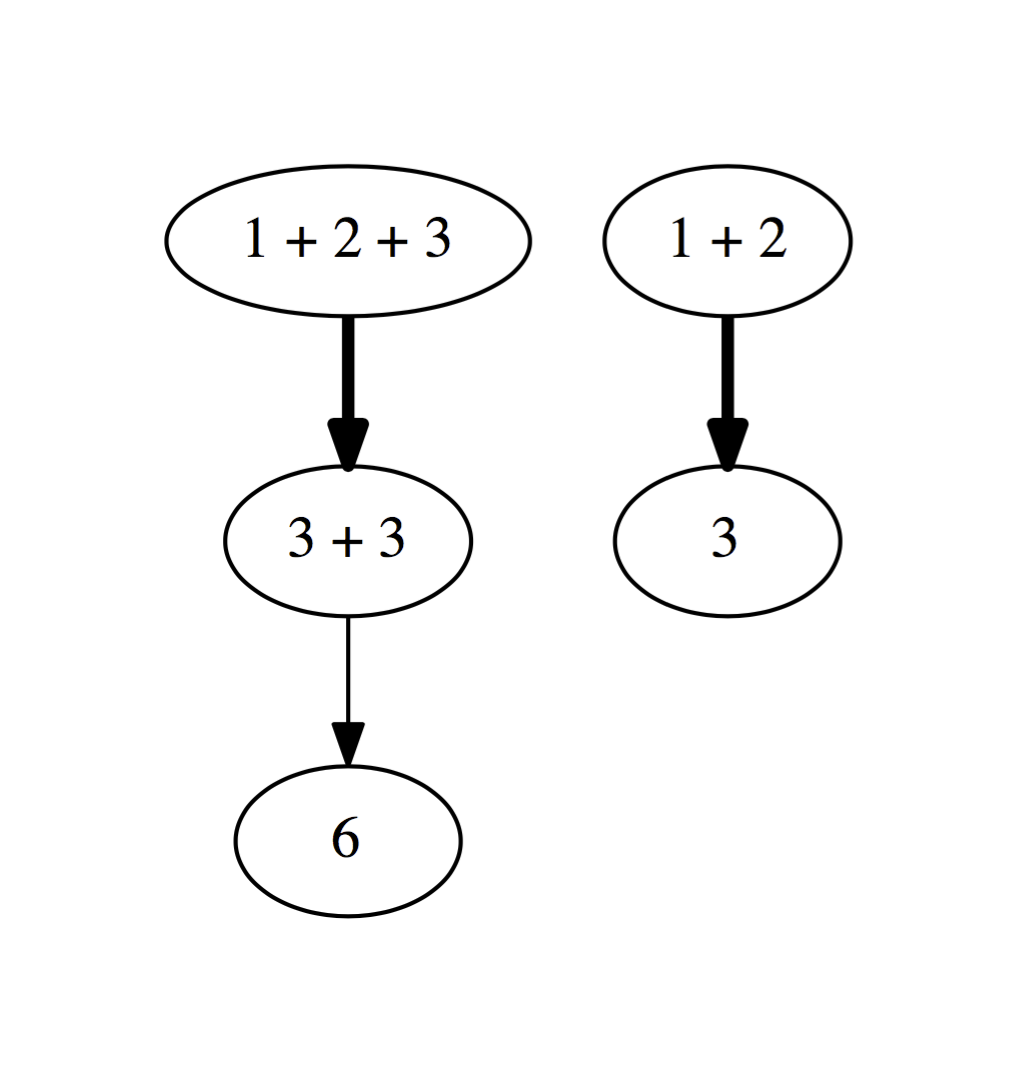
\includegraphics[width=\linewidth]{simple.png}
% \caption{The reduction graph for \texttt{1 + 2 + 3}.}
% \label{fig:simple-reduction}
% \end{figure}
% %
% We choose this graph representation instead of a simple, linear sequence
% of expressions because it will allow us to express a variety of
% traversals, such as ``step into'' and ``step over'' -- commonly found in
% traditional debuggers.



\subsection{Tracing Semantics}
\label{sec:inter-semant}
%
\begin{figure*}[t]
% \relDescription{Trace Syntax}
% $$
% \begin{array}{rrcl}
  % & \tr & ::= & \bullet \spmid \singlestep{e}{e}; \tr \spmid \subterm{e}{e}; \tr
% \end{array}
% $$
% \\
\relDescription{Computing Sub-Terms}
\begin{gather*}
\begin{array}{lcl}
\subtermssym                 & \dcolon & e \to \tr \\
\subterms{\eapp{e_1}{e_2}}   & \defeq & \subterm{\eapp{e_1}{e_2}}{e_1}; \subterm{\eapp{e_1}{e_2}}{e_2} \\
\subterms{\eplus{e_1}{e_2}}   & \defeq & \subterm{\eplus{e_1}{e_2}}{e_1}; \subterm{\eplus{e_1}{e_2}}{e_2} \\
\subterms{\eif{e_1}{e_2}{e_3}}   & \defeq & \subterm{\eif{e_1}{e_2}{e_3}}{e_1}; \\
                                &        & \subterm{\eif{e_1}{e_2}{e_3}}{e_2}; \\
                                &        & \subterm{\eif{e_1}{e_2}{e_3}}{e_3} \\
\subterms{\elet{x}{e_1}{e_2}}   & \defeq & \subterm{\elet{x}{e_1}{e_2}}{e_1}; \\
                                &        & \subterm{\elet{x}{e_1}{e_2}}{e_2} \\
\subterms{\efun{x}{e}}       & \defeq & \subterm{\efun{x}{e}}{e} \\
\subterms{e}                 & \defeq & \bullet
\end{array}
\end{gather*}
\judgementHead{Traced Evaluation}{\stepg{e}{\su}{\tr}{e}{\su}{\tr}}
\begin{gather*}
\inference[\recontext]
  {\stepg{e}{\su}{\tr}{e_1}{\su_1}{\tr_1}}
  {\stepg{C[e]}{\su}{\tr}{C[e_1]}{\su_1}{\singlestep{C[e]}{C[e_1]}; \subterms{C[e_1]}; \tr_1}}
\\ \\
\inference[\reappgood]
  {\pair{\efun{x}{e}}{\su_2} = \force{v_1}{\tfun{\thole{}}{\thole{}}}{\su_1}}
  {\stepg{\eapp{v_1}{v_2}}{\su_1}{\tr}
         {e\sub{x}{v_2}}{\su_1;\su_2}{\singlestep{\eapp{v_1}{v_2}}{e\sub{x}{v_2}}; \subterms{e\sub{x}{v_2}}; \tr}}
\\ \\
\inference[\reappbad]
  {\pair{\stuck}{\su_2} = \force{v_1}{\tfun{\thole{}}{\thole{}}}{\su_1}}
  {\stepg{\eapp{v_1}{v_2}}{\su_1}{\tr}{\stuck}{\su_1;\su_2}{\singlestep{\eapp{v_1}{v_2}}{\stuck}; \tr}}
\end{gather*}
\caption{A selection of the operational semantics from
  Figure~\ref{fig:operational}, extended to collect a full reduction
  graph.}
\label{fig:interactive}
\end{figure*}

\paragraph{Reduction Graphs}
%
A \emph{steps-to} edge is a pair of expressions \singlestep{e_1}{e_2}, which
intuitively indicates that $e_1$ steps, in a single step, to $e_2$.
%
A \emph{sub-term} edge is a pair of expressions \subterm{e_1}{e_2}, which
intuitively indicates that $e_1$ contains $e_2$ as a sub-expression.
%
A \emph{reduction graph} is a set of edges:
$$\tr ::= \bullet \spmid \singlestep{e}{e}; \tr \spmid \subterm{e}{e}; \tr$$

\paragraph{Tracing Semantics}
%
We extend the transition relation (\S~\ref{sec:semantics}) to
collect the set of edges corresponding to the reduction graph.
%
Concretely, we extend the operational semantics to
a relation of the form $\stepg{e}{\vsu}{\tr}{e'}{\vsu'}{\tr'}$
where $\tr'$ collects the edges of the transition.

\paragraph{Collecting Edges}
%
Next, we describe the general recipe for extending a transition
rule to collect edges, and provide a selection of examples
in Figure~\ref{fig:interactive}.
%
The steps-to edges are collected by recording the consequent of
each original rule in the trace. That is, each original judgment
\step{e}{\vsu}{e'}{\vsu'} becomes
\stepg{e}{\vsu}{\tr}{e'}{\vsu'}{\singlestep{e}{e'}; \tr}.
%
The sub-term edges are delegated to a helper function \subtermssym\
which adds edges from an expression to each of its
\emph{immediate} sub-expressions.
%
We collect \subtermssym edges after each transition,
to get the following template for the small-step relation:
\[
\stepg{e}{\vsu}{\tr}{e'}{\vsu'}{\singlestep{e}{e'}; \subterms{e'}; \tr}
\]

% After evaluation the reduction graph can be constructed directly from
% the trace $\tr$ as follows:
% \[
% G(\tr) = \pair{\{e \spmid e \in \tr\}}{\tr}
% \]

% \subsection{Traversing the Reduction Graph}
\subsection{Interactive Debugging}
\label{sec:traversing-graph}

Next, we show how to build a visual interactive debugger
from the traced semantics, by describing the visualization
\emph{state} \ie\ what the user sees at any given moment,
the set of \emph{commands} available to user and what
they do, and finally how we use a command to \emph{update}
the visualization state. In the sequel, for clarity of
exposition, we assume we have a (global) trace:
$\stepg{e_0}{\emptysu}{\bullet}{e_n}{\_}{\tr}$, where
$e_0$ and $e_n$ are the \emph{initial} and \emph{final}
expressions respectively.

\paragraph{Visualization State}
%
A \emph{visualization state} @VState@ is a \emph{directed graph}
whose vertices are expressions and whose edges are such
that each vertex has at most one predecessor and at most one
successor. In other words, the visualization state looks
like a set of linear lists of expressions as shown in Figure~\ref{fig:nanomaly-factorial}.
%
The \emph{initial state} is the graph containing a single
edge linking the initial and final expressions.

\paragraph{Commands}
Our debugger supports the following \emph{commands}, each of which
is parameterized by a single expression (vertex) selected from the
(current) visualization state:
%
\begin{itemize}
%
\item \stepforwardsym, \stepbackwardsym:
      show result of a single step forward or backward respectively,
%
\item \jumpforwardsym:
      show result of taking multiple steps (a \emph{``big''} step)
      upto the first beta-reduction forward or backward respectively,
%
\item \stepintosym:
      show result of stepping into a function call in a sub-term,
      isolating it from the context,

\item \stepoversym:
      show result of skipping over a function call in a sub-term.
\end{itemize}

%\begin{figure}[t]
\centering
% \begin{minipage}{0.49\linewidth}
\begin{mcode}
(*\putBefore*) :: (*\vstate*) -> (*\expr*) -> (*\expr*) -> (*\vstate*)
(*\putAfter*)  :: (*\vstate*) -> (*\expr*) -> (*\expr*) -> (*\vstate*)
(*\putRoot*)   :: (*\vstate*) -> (*\expr*) -> (*\vstate*)
(*\getRoot*)   :: (*\vstate*) -> (*\expr*) -> (*\expr*)
(*\getPath*)      :: (*\tr*) -> (*\expr*) -> [(*\expr*)]

(*\getSubterms*) :: (*\vstate*) -> (*\expr*) -> [((*\expr*),(*\ctx*))]
(*\applyCtx*)    :: (*\vstate*) -> (*\expr*) -> (*\ctx*) -> (*\expr*)

findApp    :: (*\vstate*) -> (*\expr*) -> Maybe ((*\expr*),(*\ctx*))
findValue  :: (*\vstate*) -> (*\expr*) -> (*\expr*)

data (*\cmd*) = (*\stepforwardc*) | (*\stepbackwardc*)
         | (*\jumpforwardc*) | (*\jumpbackwardc*)
         | (*\stepoverc*)    | (*\stepintoc*)
\end{mcode}
% data (*\ctx*)
\caption{Graph manipulation and traversal API.}
\label{fig:graph-api}
\end{figure}
% \end{minipage}
% \begin{minipage}{0.49\linewidth}
\begin{figure}[t]
\begin{mcode}
(*\findExpr*) :: (*\vstate*) -> (*\cmd*) -> (*\expr*) -> Maybe (*\expr*)
(*\findExpr*) v c e = case c of
  (*\stepforwardc*) -> 
    let p = (*\getPath*) v e in (p!!1)
  (*\stepbackwardc*) -> 
    let p = (*\getPath*) v ((*\getRoot*) v e) in last p
  (*\jumpforwardc*) -> case (*\findExpr*) v (*\stepforwardc*) e of
    $\eapp{v_1}{v_2}$ -> Just ($\eapp{v_1}{v_2}$)
    e'   -> (*\findExpr*) v c e'
  (*\jumpbackwardc*) -> case (*\findExpr*) v (*\stepbackwardc*) e of
    $\eapp{v_1}{v_2}$ -> Just ($\eapp{v_1}{v_2}$)
    e'   -> (*\findExpr*) v c e'
  (*\stepintoc*) -> findApp v e
  (*\stepoverc*) -> case findApp v e of
    Nothing       -> Nothing
    Just (e', cx) -> applyCtx v (crunch v e') cx

(*\updState*) :: (*\vstate*) -> (*\cmd*) -> (*\expr*) -> Maybe (*\vstate*)
(*\updState*) v c e = case (*\findExpr*) v c e of
  Nothing -> Nothing
  Just e' -> Just (*\$*) case c of
    (*\stepforwardc*) -> (*\putAfter\ v e e'*)
    (*\stepbackwardc*)    -> (*\putBefore\ v e e'*)
    (*\jumpforwardc*) -> (*\putAfter\ v e e'*)
    (*\jumpbackwardc*)    -> (*\putBefore\ v e e'*)
    (*\stepintoc*)    -> (*\putRoot\ v e' (crunch v e') *)
    (*\stepoverc*)    -> (*\putAfter\ v e e'*)
\end{mcode}
% \end{minipage}
% \[
% \begin{array}{lcl}
% \stepforward{G}{p}{e_i}  &\defeq& \left\{\begin{array}{ll}
%     e_j, & \text{where } \singlestep{e_i}{e_j} \in G
%                          \end{array}\right\} \\ \\
% \stepbackward{G}{p}{e_i}  &\defeq& \left\{\begin{array}{ll}
%     e_j, & \text{where } \singlestep{e_j}{e_i} \in G \text{ and } e_j \in p
%                          \end{array}\right\} \\ \\
% \jumpforward{G}{p}{e_i} &\defeq& \text{let } e_j = \stepforward{G}{p}{e_i} \text{ in }
%                          \left\{\begin{array}{ll}
%                          e_j, & \text{if } e_j = \eapp{v_1}{v_2} \\
%                          \jumpforward{G}{p}{e_{j}}, & \text{otherwise}
%                          \end{array}\right\} \\ \\
% \jumpbackward{G}{p}{e_i} &\defeq& \text{let } e_j = \stepbackward{G}{p}{e_i} \text{ in }
%                          \left\{\begin{array}{ll}
%                          e_j, & \text{if } e_j = \eapp{v_1}{v_2} \\
%                          \jumpbackward{G}{p}{e_{j}}, & \text{otherwise}
%                          \end{array}\right\} \\ \\
% \stepinto{G}{p}{e_i} &\defeq& \left\{\begin{array}{ll}
%                          e\sub{x}{v_2}, & \text{if } e_i = C[\eapp{v_1}{v_2}] \text{ and } \singlestep{\eapp{v_1}{v_2}}{e\sub{x}{v_2}}
%                          \end{array}\right\} \\ \\
% \stepover{G}{p}{e_i} &\defeq& \left\{\begin{array}{ll}
%                          C[v], & \text{if } e_i = C[\eapp{v_1}{v_2}] \text{ and } \multistep{\eapp{v_1}{v_2}}{v}
%                          \end{array}\right\}
% \end{array}
% \]
\caption{Rules for updating the reduction graph given a command and a selected expression. \texttt{updState} returns \texttt{Nothing} if the command was not applicable. % \stepintosym and \stepoversym require a traversal of the
  % sub-term edges to decompose $e_i$ into the target expression
  % \eapp{v_1}{v_2} and the context $C$.  \ES{these rules are quite ugly and waste space..}
}
\label{fig:traversing-graph}
\end{figure}

\begin{figure*}[t]
\[
\begin{array}{lcl}
\stepforward{G}{p}{e_i}  &\defeq& \begin{array}{ll}
    e_j, & \text{where } \singlestep{e_i}{e_j} \in G
                         \end{array}\right\} \\ \\
\stepbackward{G}{p}{e_i}  &\defeq& \left\{\begin{array}{ll}
    e_j, & \text{where } \singlestep{e_j}{e_i} \in G \text{ and } e_j \in p
                         \end{array}\right\} \\ \\
\jumpforward{G}{p}{e_i} &\defeq& \text{let } e_j = \stepforward{G}{p}{e_i} \text{ in }
                         \left\{\begin{array}{ll}
                         e_j, & \text{if } e_j = \eapp{v_1}{v_2} \\
                         \jumpforward{G}{p}{e_{j}}, & \text{otherwise}
                         \end{array}\right\} \\ \\
\jumpbackward{G}{p}{e_i} &\defeq& \text{let } e_j = \stepbackward{G}{p}{e_i} \text{ in }
                         \left\{\begin{array}{ll}
                         e_j, & \text{if } e_j = \eapp{v_1}{v_2} \\
                         \jumpbackward{G}{p}{e_{j}}, & \text{otherwise}
                         \end{array}\right\} \\ \\
\stepinto{G}{p}{e_i} &\defeq& \left\{\begin{array}{ll}
                         e\sub{x}{v_2}, & \text{if } e_i = C[\eapp{v_1}{v_2}] \text{ and } \singlestep{\eapp{v_1}{v_2}}{e\sub{x}{v_2}}
                         \end{array}\right\} \\ \\
\stepover{G}{p}{e_i} &\defeq& \left\{\begin{array}{ll}
                         C[v], & \text{if } e_i = C[\eapp{v_1}{v_2}] \text{ and } \multistep{\eapp{v_1}{v_2}}{v}
                         \end{array}\right\}
\end{array}
\]
\caption{Rules for updating the reduction graph given a command and a selected expression. \texttt{updState} returns \texttt{Nothing} if the command was not applicable. % \stepintosym and \stepoversym require a traversal of the
  % sub-term edges to decompose $e_i$ into the target expression
  % \eapp{v_1}{v_2} and the context $C$.  \ES{these rules are quite ugly and waste space..}
}
\label{fig:traversing-graph}
\end{figure*}


\paragraph{Update}
Figure~\ref{fig:traversing-graph} shows how we update the state
for each command.
%
The procedure @findExpr vs cmd e@ traverses $\tr$
and the current visualization state to compute the new
expression that should be added to the visualization state,
and @updState vs cmd e@ then updates the graph
by inserting the new expression appropriately, using one of
the following functions.
%
@putBefore vs e e'@ \hbox{(resp. @putAfter vs e e'@)}
returns the modified version of @vs@ where @e'@ is the
immediate predecessor of @e@ (resp. the immediate successor of @e@);
%
@putRoot vs e e'@ returns the modified version of @vs@ extended
with a new root vertex @e@ and its successor @e'@.
%
% @getRoot vs e@ returns the vertex (expression) obtained
% by transitively following the predecessors of @e@ until a
% source vertex.

@getNext vs e@ returns the immediate successor of @e@ in $\tr$.
%
@getPrev vs e@ computes the path @p@ between @e@ and its immediate
predecessor in the current visualization, and then returns @e@'s immediate
predecessor along @p@.
%
@getSubterms vs e@ traverses the sub-term edges to decompose an
expression into a list of sub-expressions paired with their context.
%
@applyCtx vs e ctx@ applies @ctx@ to @e@, traversing the sub-term edges
in reverse to find the super-term of @e@.
%
\hbox{@findApp vs e@} builds on top of @getSubterms@ to find the first
application sub-term (if any), \ie the first sub-term that looks like
$\eapp{v_1}{v_2}$.
%
@findVal vs e@ traverses the single-step edges to find the final value
that @e@ reduces to.
%
% Note that the sub-term edges $\searrow$ allow us to decompose an
% expression into a sub-expression and the surrounding context, thus
% enabling the \stepintosym\ and \stepoversym\ traversals.

% \RJ{EXAMPLE of interaction from overview goes here}
\begin{figure}[t]
\centering
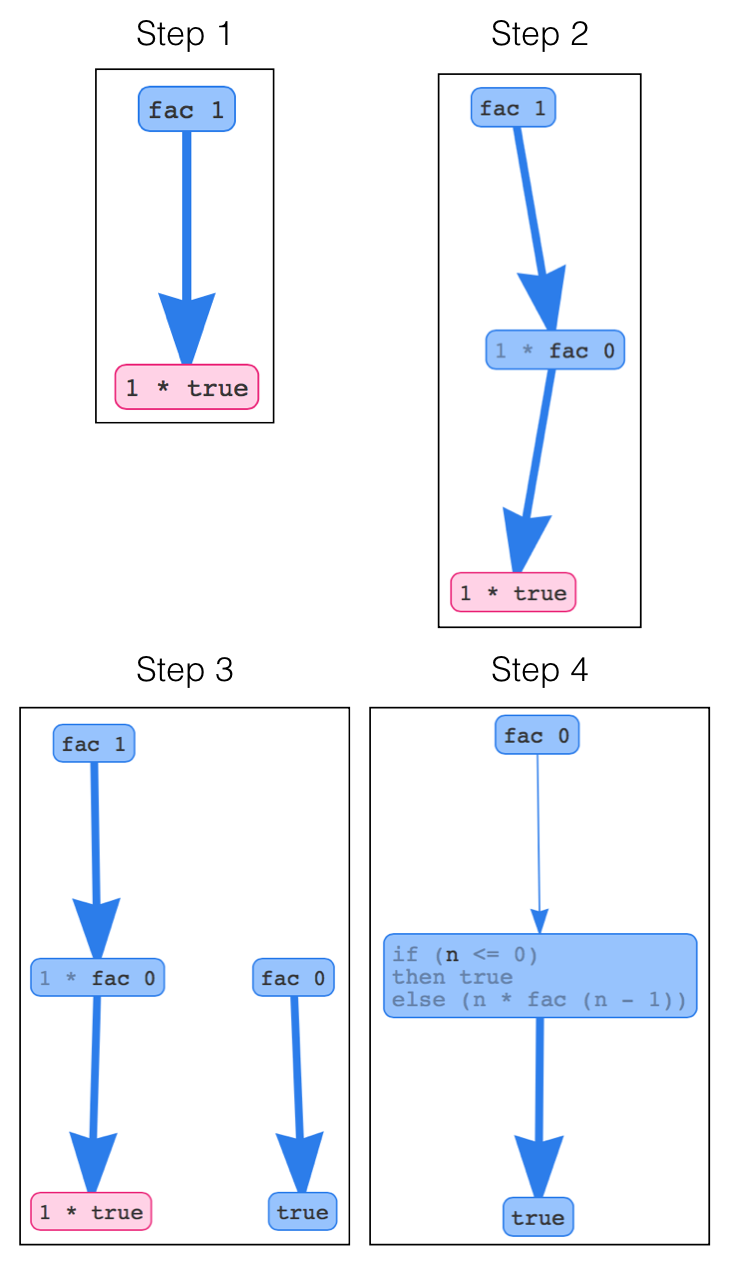
\includegraphics[width=0.8\linewidth]{fac-steps.png}
\caption{A sequence of interactions with the trace of
  \texttt{fac 1}. The stuck term is red, in each node the redex is
  highlighted. Thick arrows denote a multi-step transition, thin arrows
  denote a single-step transition. We start in step 1. In step 2 we jump
  forward from the witness to the next function call. In step 3 we step
  into the recursive \texttt{fac 0} call, which spawns a new ``thread''
  of execution. In step 4 we take a single step forward from
  \texttt{fac 0}.} % (hiding the context for space).}
\label{fig:nanomaly-factorial}
\end{figure}

%
%
%The initial path $p$ is required for the backward-steps as a node may
%have multiple incoming $\leadsto$ edges, \eg
%\singlestep{\eplus{1}{2}}{3} and \singlestep{\eplus{2}{1}}{3}.
%

}


\end{document}
